% Copyright (C) 2014-2017 by Thomas Auzinger <thomas@auzinger.name>

\documentclass[draft,final]{vutinfth} % Remove option 'final' to obtain debug information.

% Load packages to allow in- and output of non-ASCII characters.
\usepackage{lmodern}        % Use an extension of the original Computer Modern font to minimize the use of bitmapped letters.
\usepackage[T1]{fontenc}    % Determines font encoding of the output. Font packages have to be included before this line.
\usepackage[utf8]{inputenc} % Determines encoding of the input. All input files have to use UTF8 encoding.

% Extended LaTeX functionality is enables by including packages with \usepackage{...}.
\usepackage{amsmath}    % Extended typesetting of mathematical expression.
\usepackage{amssymb}    % Provides a multitude of mathematical symbols.
\usepackage{mathtools}  % Further extensions of mathematical typesetting.
\usepackage{microtype}  % Small-scale typographic enhancements.
%\usepackage[inline]{enumitem} % User control over the layout of lists (itemize, enumerate, description).
\usepackage{multirow}   % Allows table elements to span several rows.
\usepackage{booktabs}   % Improves the typesettings of tables.
\usepackage{subcaption} % Allows the use of subfigures and enables their referencing.
\usepackage[ruled,linesnumbered,algochapter]{algorithm2e} % Enables the writing of pseudo code.
\usepackage[usenames,dvipsnames,table]{xcolor} % Allows the definition and use of colors. This package has to be included before tikz.
\usepackage{nag}       % Issues warnings when best practices in writing LaTeX documents are violated.
\usepackage{todonotes} % Provides tooltip-like todo notes.
\usepackage{hyperref}  % Enables cross linking in the electronic document version. This package has to be included second to last.


\usepackage{morewrites}

\usepackage[newfloat]{minted}
\usepackage{caption}

\usepackage{pgfplots}
\pgfplotsset{compat=1.8}
\usepgfplotslibrary{statistics}

\newenvironment{code}{\captionsetup{type=listing}}{}
\SetupFloatingEnvironment{listing}{name=Listing}

%\usepackage{listings}
%\lstset{
%	language=bash,
%	basicstyle=\footnotesize, 
%	breakatwhitespace=false,
%	escapeinside={\%*}{*)}
%}
\usepackage[nonumberlist,acronym,section=section]{glossaries} % Enables the generation of glossaries and lists fo acronyms. This package has to be included last.
% Define convenience functions to use the author name and the thesis title in the PDF document properties.
\newcommand{\authorname}{Bernhard Gößwein} % The author name without titles.
\newcommand{\thesistitle}{Designing a Framework gaining Repeatability for the openEO platform} % The title of the thesis. The English version should be used, if it exists.

% Set PDF document properties
\hypersetup{
    pdfpagelayout   = TwoPageRight,           % How the document is shown in PDF viewers (optional).
    linkbordercolor = {Melon},                % The color of the borders of boxes around crosslinks (optional).
    pdfauthor       = {\authorname},          % The author's name in the document properties (optional).
    pdftitle        = {\thesistitle},         % The document's title in the document properties (optional).
    pdfsubject      = {Subject},              % The document's subject in the document properties (optional).
    pdfkeywords     = {a, list, of, keywords} % The document's keywords in the document properties (optional).
}

\setpnumwidth{2.5em}        % Avoid overfull hboxes in the table of contents (see memoir manual).
\setsecnumdepth{subsection} % Enumerate subsections.

\nonzeroparskip             % Create space between paragraphs (optional).
\setlength{\parindent}{0pt} % Remove paragraph identation (optional).

\makeindex      % Use an optional index.
\makeglossaries % Use an optional glossary.
%\glstocfalse   % Remove the glossaries from the table of contents.

% Set persons with 4 arguments:
%  {title before name}{name}{title after name}{gender}
%  where both titles are optional (i.e. can be given as empty brackets {}).
\setauthor{}{\authorname}{}{male}
\setadvisor{Ao.Univ.Prof. Dipl.-Ing. Dr.techn.}{Andreas Rauber}{}{male}

% For bachelor and master theses:
%\setfirstassistant{Ao.Univ.Prof. Dipl.-Ing. Dr.techn.}{Andreas Rauber}{}{male}
\setfirstassistant{Dr.}{Tomasz Miksa}{}{male}
%\setthirdassistant{Pretitle}{Forename Surname}{Posttitle}{male}

% For dissertations:
%\setfirstreviewer{Pretitle}{Forename Surname}{Posttitle}{male}
%\setsecondreviewer{Pretitle}{Forename Surname}{Posttitle}{male}

% For dissertations at the PhD School and optionally for dissertations:
%\setsecondadvisor{Pretitle}{Forename Surname}{Posttitle}{male} % Comment to remove.

% Required data.
\setaddress{Vorderer Ödhof 1, 3062 Kirchstetten}
\setregnumber{01026884}
\setdate{01}{08}{2019} % Set date with 3 arguments: {day}{month}{year}.
\settitle{\thesistitle}{Entwurf eines Frameworks zur Unterstützung von Reproduzierbarkeit für die openEO Plattform} % Sets English and German version of the title (both can be English or German). If your title contains commas, enclose it with additional curvy brackets (i.e., {{your title}}) or define it as a macro as done with \thesistitle.
\setsubtitle{}{} % Sets English and German version of the subtitle (both can be English or German).

% Select the thesis type: bachelor / master / doctor / phd-school.
% Bachelor:
%\setthesis{bachelor}
%
% Master:
\setthesis{master}
\setmasterdegree{dipl.} % dipl. / rer.nat. / rer.soc.oec. / master
%
% Doctor:
%\setthesis{doctor}
%\setdoctordegree{rer.soc.oec.}% rer.nat. / techn. / rer.soc.oec.
%
% Doctor at the PhD School
%\setthesis{phd-school} % Deactivate non-English title pages (see below)

% For bachelor and master:
\setcurriculum{Software Engineering and Internet Computing}{Software Engineering and Internet Computing} % Sets the English and German name of the curriculum.

% For dissertations at the PhD School:
%\setfirstreviewerdata{Affiliation, Country}
%\setsecondreviewerdata{Affiliation, Country}
\newcounter{tmp@cnt}

\newcommand{\bgoesswe}[1]{#1}
\newcommand{\bgoesswein}[1]{{\color{blue}#1}}
\newcommand{\bgoessweindel}[1]{{\color{red}#1}}

\newcommand*\combine[1][2]{%
	\refstepcounter{enumi}
	\setcounter{tmp@cnt}{\value{enumi}}
	\addtocounter{enumi}{#1-1}
	\item[\thetmp@cnt--\theenumi\@labelpunc]}

\newcolumntype{L}[1]{>{\centering\arraybackslash}l{#1}}

\newacronym{api}{API}{Application Programming Interface}
\newacronym{gee}{GEE}{Google Earth Engine}
\newacronym{eodc}{EODC}{Earth Observation Data Centre}
\newacronym{soa}{SOA}{Service Oriented Architecture}
\newacronym{esa}{ESA}{European Space Agency}
\newacronym{ndvi}{NDVI}{Normalized Difference Vegetation Index}
\newacronym{pid}{PID}{Persistent Identifier}
\newacronym{openeo}{openEO}{Open Source Earth Observation Project}
\newacronym{rda}{RDA}{Research Data Alliance}
\newacronym{primad}{PRIMAD}{\textbf{P}latform \textbf{R}esearch \textbf{O}bjectives \textbf{I}mplementation \textbf{M}ethods \textbf{A}ctors \textbf{D}ata model}
\newacronym{wgdc}{WGDC}{Working Group on Data Citation}
\newacronym{vzj}{VZJ}{Vadose Zone Journal}
\newacronym{rr}{RR}{Reproducible Research}
\newacronym{gpf}{GPF}{Geoscience Paper of the Future}
\newacronym{ccca}{CCCA}{Climate Change Centre Austria}
\newacronym{netcdf}{NetCDF}{Network Common Data Form}
\newacronym{geotiff}{GeoTiff}{Georeferenced Tagged Image File Format}
\newacronym{tds}{TDS}{Thredds Data Server}
\newacronym{xml}{XML}{Extensible Markup Language}
\newacronym{geobia}{GEOBIA}{Geographic Object-Based Image Analysis}
\newacronym{obia}{OBIA}{Object-Based Image Analysis}
\newacronym{vcs}{VCS}{Version Control Systems}
\newacronym{sha}{SHA}{Secure Hash Algorithm}
\newacronym{rest}{REST}{Representational State Transfer}
\newacronym{json}{JSON}{JavaScript Object Notation}
\newacronym{ogc}{OGC}{Open Geospatial Consortium}
\newacronym{csw}{CSW}{Catalogue Service for the Web}
\newacronym{udf}{UDF}{User Defined Functions}
\newacronym{eo}{EO}{Earth Observation}
\newacronym{cli}{CLI}{Command Line Interface}
\newacronym{cpu}{CPU}{Central Processing Unit}
\newacronym{gpu}{GPU}{Graphics Processing Unit}
\newacronym{ram}{RAM}{Random Access Memory}
\newacronym{os}{OS}{Operating System}

\newglossaryentry{backend}
{
	name={backend},
	description={A web service provider, capable of processing and providing geoscientific data}
}

\newglossaryentry{job}
{
	name={job},
	description={Definition of a workflow execution on a backend, including the input data}
}

\newglossaryentry{process}
{
	name={process},
	description={Algorithm that gets executed over earth observation data. May use the output of another process as input data}
}

\newglossaryentry{processgraph}
{
	name={process graph},
	description={openEO definition of a job in a JSON format}
}

\newglossaryentry{experiment}
{
	name={experiment},
	description={Practical scientific earth observation research using at least one backend with at least one job}
}

\newglossaryentry{workflow}
{
	name={workflow},
	description={Step by step description of an experiment}
}

\begin{document}

\frontmatter % Switches to roman numbering.
% The structure of the thesis has to conform to
%  http://www.informatik.tuwien.ac.at/dekanat

\addtitlepage{naustrian} % German title page (not for dissertations at the PhD School).
\addtitlepage{english} % English title page.
\addstatementpage

%\begin{danksagung*}


%\end{danksagung*}

\begin{acknowledgements*}
To my girlfriend Viola: Thank you very much for helping me through the stressful days of working on the thesis and for providing breaks and diversions when I needed them.\\ \\
To my family: Thank you for supporting me through my whole studying time and for motivating me to go on with the thesis. \\ \\
To my colleagues of the Remote sensing research group: Thank you for patiently waiting for me to finish my studies and letting me work on a thesis within the openEO project. \\ \\
To my colleagues at EODC: Thank you for providing me all resources I requested and letting me implement the solution on your system. \\ \\
Last but not least to my supervisors Andreas Rauber and Tomasz Miksa for always quickly replying to my questions and providing me with constructive feedback. 
\end{acknowledgements*}

\begin{kurzfassung}
%\todo{Neu übersetzen wenn Abstract fertig ist}
Wissenschaftler im Bereich der Erdbeobachtung verwenden spezielle rechnergestützte Services um Satellitenbilder bei externen Datenanbietern zu verarbeiten. Die zugrundeliegende Quelle der Daten ist meist ähnlich, beispielsweise werden Sentinel Satellitendaten ausschließlich von Copernicus in Zusammenarbeit der European Space Agency betrieben. Die Art der Aufbereitung, Aktualisierung, Korrektur und anschließenden Analyse kann von Anbieter zu Anbieter unterschiedlich sein. 
Die Anbieter unterstützen meist keine Datenversionierung, beispielsweise wenn Daten korrigiert werden wird dies nicht dokumentiert. Außerdem werden Änderungen in der verwendeten Software nicht kommuniziert und stellt daher eine Black Box für die Wissenschaftler dar. Daher haben Wissenschaftler die diese Systeme nutzen keine Möglichkeit herauszufinden warum die Durchführung des gleichen Programmcodes unterschiedliche Ergebnisse liefert. Dieser Umstand behindert die Reproduzierbarkeit der Experimente im Bereich der Erdbeobachtung. 
In dieser Arbeit wird gezeigt, wie existierende Datenanbieter modifiziert werden können um Reproduzierbarkeit zu ermöglichen. Die präsentierten Erweiterungen basieren auf den Empfehlungen der Reseach Data Alliance bezüglich Datenidentifizierung und auf das \bgoesswein{\mbox{VFramework}} bezüglich automatisierte Dokumentation und Identifikation der durchgeführten Prozesse. Zusätzlich werden Vorschläge dafür präsentiert wie Anbieter die gesammelten Informationen für die Wissenschaftler zur Verfügung stellt. Die Implementierung der vorgestellten Erweiterungen werden am Earth Observation Data Centre, einem Partner des openEO Projektes durchgeführt. Die Evaluierung des fertigen Systems erfolgt durch die Durchführung von typischen Szenarien der Erdwissenschaften und durch zusätzliche Tests bezüglich der Effekte der Performance- und Speicherbedarfs für das System des Anbieters. Das Ergebnis der Evaluation lässt darauf schließen, dass Reproduzierbarkeit mit nur minimalen zusätzlichen Performance- und Speicherplatzbedarf möglich ist.          
\end{kurzfassung}


\begin{abstract}
%\todo{Wichtige Kapitel: Abstract, Introduction, Conclusion, evtl. Evaluation Summary}
%\todo{Let Viola/Sophie read through it !!}
%\todo{Read through it again}
% Abstract from paper
%Earth observation researchers use specialised computing services for satellite image processing offered by various data backends. The source of data is often the same, for example Sentinel-2 satellites operated by the European Space Agency, but the way how data is pre-processed, corrected, updated, and later analysed may differ among the backends.
%Backends often lack mechanisms for data versioning, for example, data corrections are not tracked. Furthermore, an evolving software stack used for data processing remains a black box to researchers. Researchers have no means to identify why executions of the same code deliver different results. This hinders reproducibility of  earth observation experiments.
%In this paper, we present how infrastructure of existing earth observation data backends can be modified to support reproducibility. The proposed extensions are based on recommendations of the Research Data Alliance regarding data identification and the VFramework for automated process provenance documentation. We implemented these extensions at the Earth Observation Data Centre, a partner in the openEO consortium. We evaluated the solution on a variety of usage scenarios, providing also performance and storage measures to evaluate the impact of the modifications. The results indicate reproducibility can be supported with minimal performance and storage overhead.

Earth observation researchers use specialised computing services for satellite image processing offered by various data backends. The source of data is similar, for example Sentinel satellites operated by Copernicus and the European Space Agency. The way it is pre-processed, updated, corrected and later analysed may differ among the backends.
Backends often lack mechanisms for data versioning, for example, data corrections are not tracked. Furthermore, an evolving software stack used for data processing remains a black box to researchers. Researchers have no means to identify why executions of the same code deliver different results. This hinders reproducibility of earth observation experiments.
In this thesis, we present how existing earth observation backends can be modified to support reproducibility. The proposed extensions are based on recommendations of the Research Data Alliance regarding data identification and the VFramework for automated process provenance documentation. Additionally, we provide suggestions on how backends make the captured information accessable for scientists. We implemented these extensions at the Earth Observation Data Centre, a partner in the openEO consortium. We evaluated the solution on a variety of usage scenarios, providing also performance and storage measures to evaluate the impact of the modifications. The results indicate reproducibility can be supported with minimal performance and storage overhead.     
\end{abstract}

% Select the language of the thesis, e.g., english or naustrian.
\selectlanguage{english}

% Add a table of contents (toc).
\tableofcontents % Starred version, i.e., \tableofcontents*, removes the self-entry.

% Switch to arabic numbering and start the enumeration of chapters in the table of content.
\mainmatter

\chapter{Introduction}\label{Introduction}

\section{Motivation}\label{Motivation}\label{Use Cases}
% Background
\gls{eo} sciences gathers images of the Earth's surface and atmosphere using instruments and cameras on aircrafts or satellites. Advancing technologies in space agencies lead to the usage of mostly satellite images. The data is too big to be downloaded for local analysis. The solution is to store it in high-performance computational backends, process it there, and browse the results or download resulting figures or numbers. The vast majority of backends are available via \gls{soa} interfaces. Data providers like \gls{gee}\footnote{https://earthengine.google.com} and \gls{eodc}\footnote{https://www.eodc.eu} host a Web \gls{api}.Scientists create a local description of the \gls{workflow} and satellite data to describe experiments. They send the description to the \gls{backend} and are notified when the processing has finished \cite{geocloud}. 

% Problem
Such an approach addresses the performance issues, but it does not allow researchers to take full control of the environment in which their experiments are executed. The backends present themselves as black boxes to the researchers with no possibility of obtaining information on environment configuration, e.g. software libraries used in processing and their versions. Studies in different domains show that the computational environment can have an impact on the reproducibility of scientific experiments and must be documented in order to ensure reproducibility \cite{Freesurfer} \cite{Thestateofreproducibility}  \cite{MiksaBiomedical}. Still the vast majority of backend providers do not share such environment information. Another problem constitutes the precise identification of data used for processing. EO backends in Europe usually obtain data from the same source, for example from the Sentinel-2 satellites operated by the European Space Agency (ESA). The data provider releases updates and corrections to the data in the case that one of the instruments used for observation was wrongly calibrated or broken and raw data had to be processed again. An example for this is the format update of \gls{esa} in 2017 of the Sentinel 1 dataset, which affected data records of the backends, see \footnote{https://sentinel.esa.int/web/sentinel/missions/sentinel-1/news/-/article/sentinel-1-update-of-product-format}. Updated data is released to backend operators. Usually there is no versioning mechanism for data. Researchers do not know which version of data was used in their study, i.e. whether they were using a version before or after some specific modification was made. This leads to the problem that scientists are not able to precisely identify and cite the input data of their experiments, which hinders reproducibility and in turn undermines trust in the results. For a better understanding of the problem we present the conclusion of two studies regarding reproducibility in EO science after defining used terms of them. \\
We define the term "reproducibility" by running a second \bgoesswein{similar} \gls{experiment}, which arrives at the same conclusion as the original experiment. \bgoessweindel{The more an additional experiment differs from an original one, the more information is gained.} It is necessary to produce evidence for the outcome of an experiment. We define the term "replicability" as the re-run of the same methods of an original experiment to show that the described methods lead to the claimed results \cite{reprovsrepli}. \\

The first study examines existing publications in the scientific EO community. It does not actively try to reproduce the experiments, but looks at the description of the methods. The aim of the paper is to give an overview of the reproducibility and replicability of the publications. The results show that only half of the publications were replicable and none of them reproducible \cite{Ostermann2017AdvancingSW}. \\
The second study intends to replicate the work of EO scientists and executes a survey of geoscientific readers and authors. Its aim is to find reasons for the lack of reproducibility in earth observation sciences. One result is that even though 49\% of the participants responded that their publications are reproducible, only 12\% of them have linked the used code. This leads to the conclusion that the understanding of open, reproducible research is different among the participating scientists. The interpretations are more in favor of own publications regarding replicability. The main findings for the lack of reproducibility in computational geoscience are listed below \cite{Thestateofreproducibility}:  

\begin{enumerate}
	\item Insufficiently described methods 
	\item No persistent data identifier
	\item Legal concerns
	\item The impression that it is not necessary
	\item Too \bgoesswein{t}ime consuming
\end{enumerate} 

The reproduction of geoscientific papers fails due to the different individual interpretations of the described approach. When the code was published with the publication, alternative software environments produced unequal results. For example different versions of the CRAN library in R created unequal results. The majority of the replication required changes of code and a deeper understanding of the procedures, for example caused by deprecated functions. System dependent issues occurred, which are related to the usage of random access memory and installation libraries of the operating system. 
The study shows an example of a problematic replication using a resulting image of a publication.
It re-executes the experiment to receive this image and compares it with the original one. Figure \ref{fig:motivation} shows a comparison of the recreated image and the original image. The map shows spatially gridded biomass burning and was published initially in \cite{bg-13-3225-2016}. Even though the resulting numbers of the reproduction remain the same, the different aspect ratio changes the appearance of the resulting image and might lead to different interpretations \cite{Thestateofreproducibility}.

\begin{figure}[h]
	\centering
	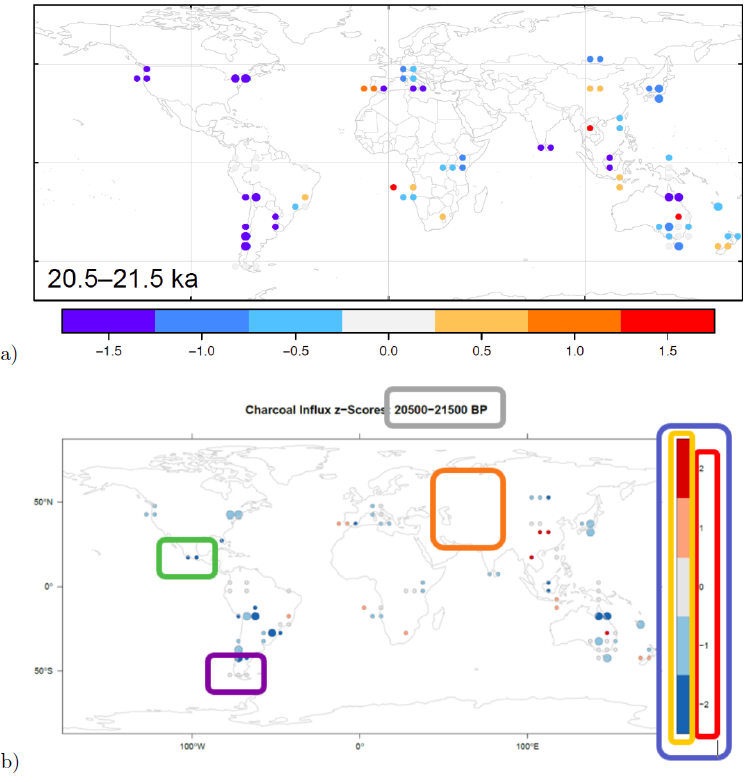
\includegraphics[scale=0.5]{motivation_example}
	\caption{Example of a comparison of the original result (a) and a replicated result (b). The boxes are highlighting the differences of the map. The blue box indicates the misplacement of the legend, the purple box shows different color of results, the red box shows a different data type of the legend numbers, the grey box shows a different labeling, the orange box highlights differences in the background map, the yellow box shows a different number of classes and the green box shows results that were not in the original figure \cite{Thestateofreproducibility}.}
	\label{fig:motivation} % \label has to be placed AFTER \caption (or \subcaption) to produce correct cross-references.
\end{figure} 

The problem description leads us to create the following three use cases to further specify the aim of the thesis. They describe scenarios focused on scientific experiments that are currently not achievable, but shall be made possible to accomplish with the solution of this thesis. This thesis uses the term \gls{job} for the definition of a description of a workflow executed at a backend since the term is common in EO sciences. The following sections describe these use cases as well as the example experiment that will be used to guide the reader through the thesis.  

\subsection{Example Experiment}\label{example}

This section describes an example of an experiment that a remote sensing scientist wants to execute. The thesis uses the example throughout the thesis for a better illustration of the concepts. They are used in the use cases as well. \\
The input data of the experiment is Sentinel 2 data developed by the ESA. The area of interest is the province of South Tyrol defined by the bounding area in the "EPSG:4326" projection with the coordinates of a north-west corner (10.288696, 46.905246) and a south-east corner (12.189331, 45.935871). The time of interest is the month of May in 2017. The scientist works on vegetation dynamics and wants to know what the state of the vegetation of South Tyrol was in May 2017. Therefore the minimum of the  \gls{ndvi}\footnote{https://earthobservatory.nasa.gov/features/MeasuringVegetation/measuring\_vegetation\_2.php} is calculated on the data selection. It derives from the difference between near-infrared (which reflects vegetation strongly) and red light (which vegetation absorbs). So for every pixel of the satellite image, the NDVI value is calculated for every day of May 2017. Then the 31 images are reduced to one by taking the minimum NDVI value of each pixel. Figure \ref{fig:example} shows the results of the running example execution.\\

The execution of this experiment consists of the following workflow:

\begin{enumerate}
	\item Selecting the Sentinel 2 data records
	\item Filtering the Sentinel 2 records by the extent of south tyrol. \\(10.288696, 46.905246) - (12.189331, 45.935871) on "EPSG:4326" projection.
	\item Filtering the Sentinel 2 records by May 2017.
	\item Calculate NDVI for all days of May 2017.
	\item Reduce by the minimum value of May 2017.
	\item Create and start a job at the backend. 
	\item Interpret the resulting image.
\end{enumerate}

\begin{figure}[h]
	\centering
	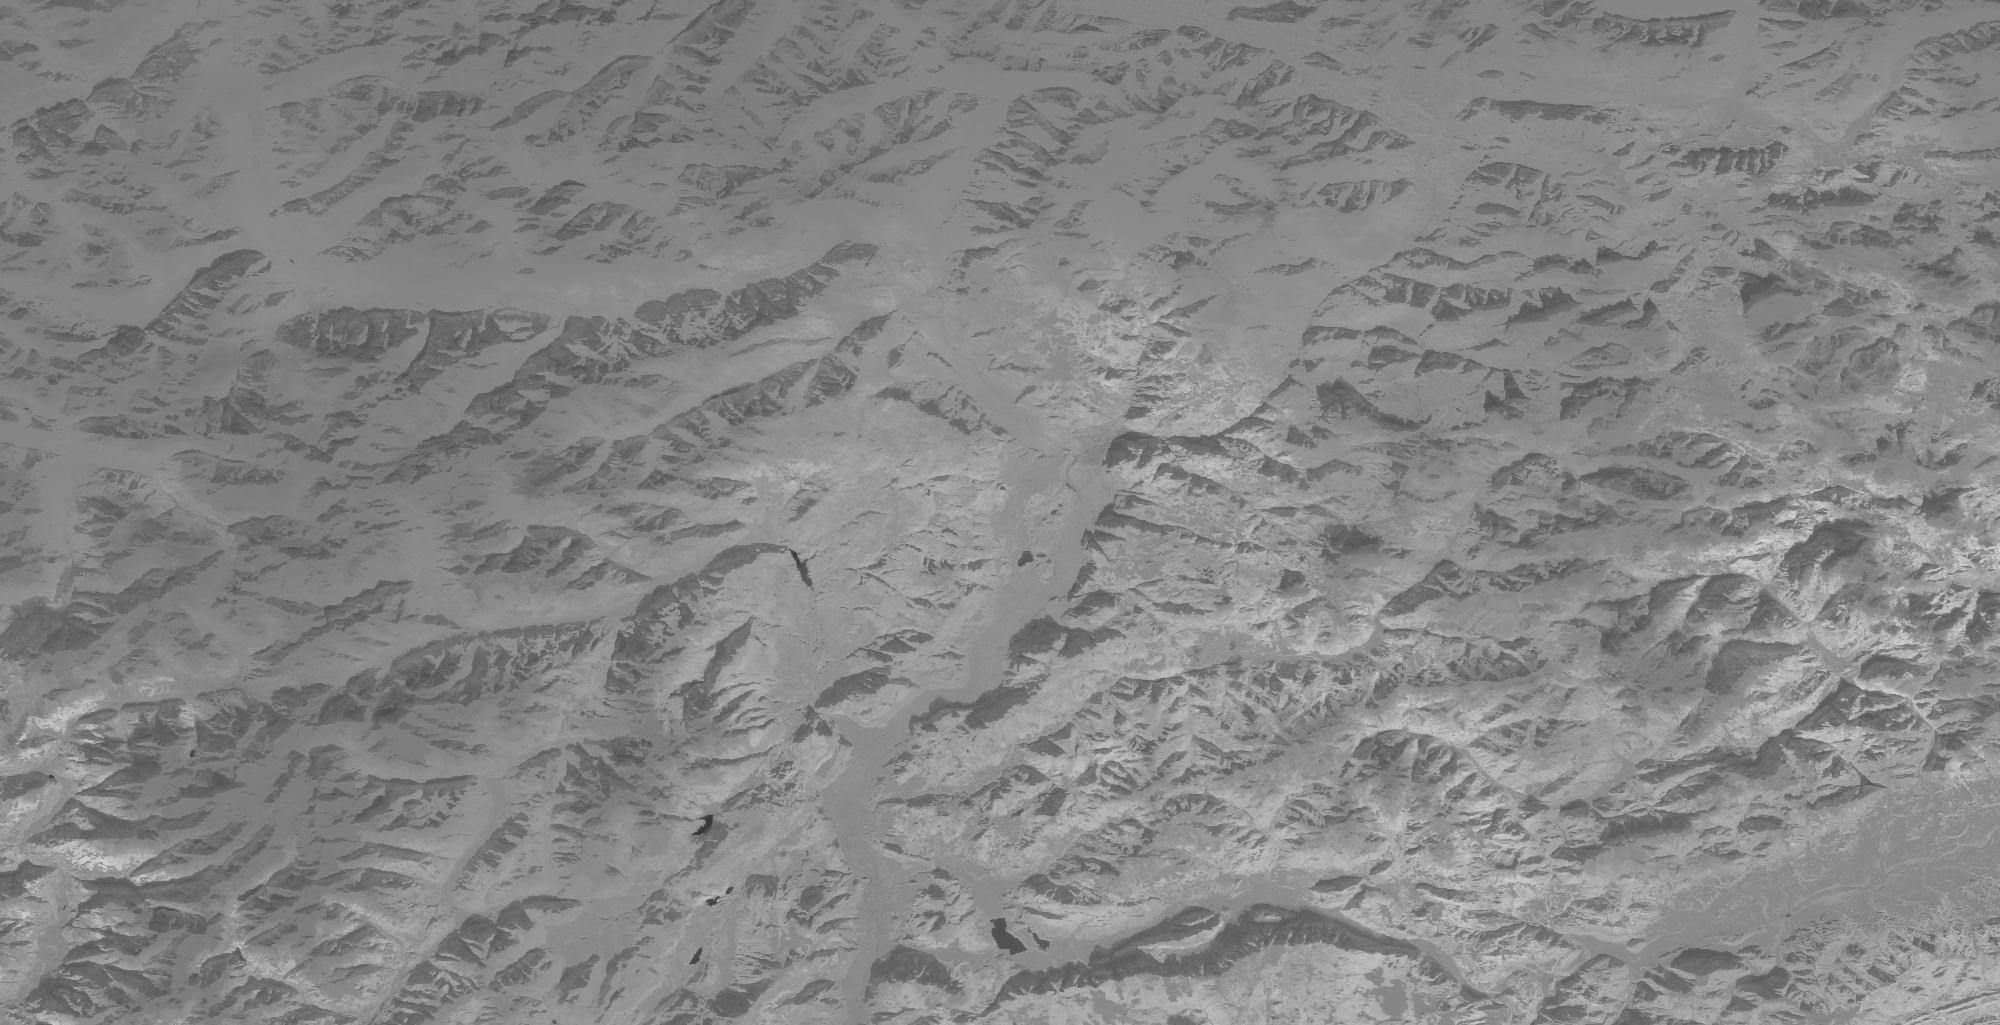
\includegraphics[width=\textwidth]{openeo_example_output}
	\caption{Resulting image of the running example.}
	\label{fig:example} % \label has to be placed AFTER \caption (or \subcaption) to produce correct cross-references.
\end{figure}


\subsection{Use Case 1 – Re-use of input data}\label{UseCase1}
\begin{figure}[h]
	\centering
	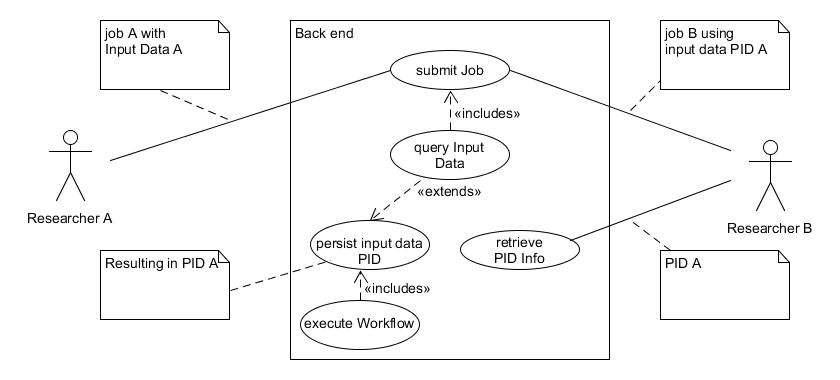
\includegraphics[width=\textwidth]{usecase1}
	\caption{Overview of the first use case: Re-use of input data}
	\label{fig:usecase1} % \label has to be placed AFTER \caption (or \subcaption) to produce correct cross-references.
\end{figure}
The first use case is concerned with the re-use of input data between job executions. Reproducible methods are important for the scientific community. Scientists are likely to build on results and methods of publications and this scenario makes the re-use easier. In this use case, a scientist wants to create a publication by running the example experiment, described in Section \ref{example} using an earth observation backend. By creating and starting the job, the backend generates a \gls{pid} for the input data of the experiment. After that, the scientist publishes the results and cites the input data with the resulting PID. It redirects to a human-readable landing page that provides meta information about the dataset. Another scientist, also interested in the vegetation of South Tyrol, wants to use the same input data but chooses a different approach of processing it (for example the maximum instead of minimum reduction function). Hence, the input data PID can be used to re-use the same data. The backend has to be capable of resolving the PID automatically to enable users to work with the same input data for a new job. The data provider needs to persist the data defined by a PID even if updates on the data take place.   

\begin{itemize}
	\item \textbf{Input Data A}: Sentinel 2 data of the area of South Tyrol in May 2017. 
	\item \textbf{Job A}: Taking the \textbf{minimum} NDVI of the area of South Tyrol in May 2017. 
	\item \textbf{Job B}: Taking the \textbf{maximum} NDVI of the area of South Tyrol in May 2017.
\end{itemize}

Figure \ref{fig:usecase1} gives an overview of the first use case. \\

The scenario sequence of actions is summarized in the following steps: \\

\begin{enumerate}
	\item Researcher A runs job A at the backend.
	\item Researcher A retrieves the used input data PID of job A.
	\item Researcher A cites the input data with the PID in a publication.
	\item Researcher B uses the same input data, by applying the data PID of job A for job B.  
\end{enumerate}

\subsection{Use Case 2 – Providing job execution information}\label{UseCase2}
\begin{figure}[h]
	\centering
	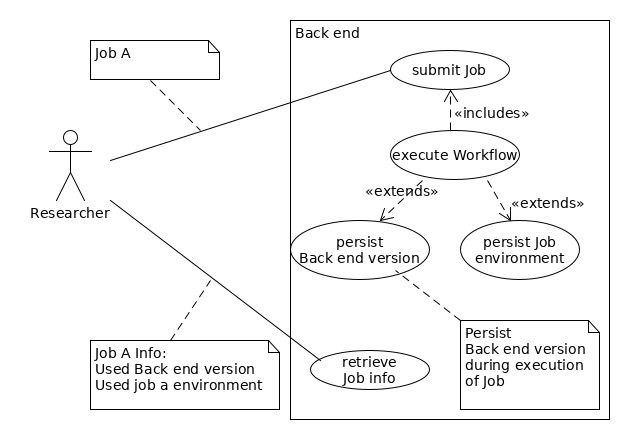
\includegraphics[width=\textwidth]{usecase2}
	\caption{Overview of the second use case: Providing job execution information}
	\label{fig:usecase2} % \label has to be placed AFTER \caption (or \subcaption) to produce correct cross-references.
\end{figure}

The second use case is similar to the first one but it is exclusively concerned with job dependent environment information. The scientist automatically gets environment data about the job execution e.g. used software packages and their versions. The motivation for this is to add transparency of the job execution for users, so that researchers can describe their processes in more detail. It helps geoscientists to understand why results differ from executions in the past. Figure \ref{fig:usecase2} gives an overview of the use case. 
The following steps summarize the scenario sequence of actions: \\
\begin{enumerate}
	\item Researcher runs a job (job A) at a backend.
	\item Researcher wants to describe the job environment.
	%	\item Back End Developer releases a new version.   
	%	\item Back End Developer runs test jobs to find differences.
\end{enumerate}

\subsection{Use Case 3 – Compare different job executions}\label{UseCase3}
\begin{figure}[h]
	\centering
	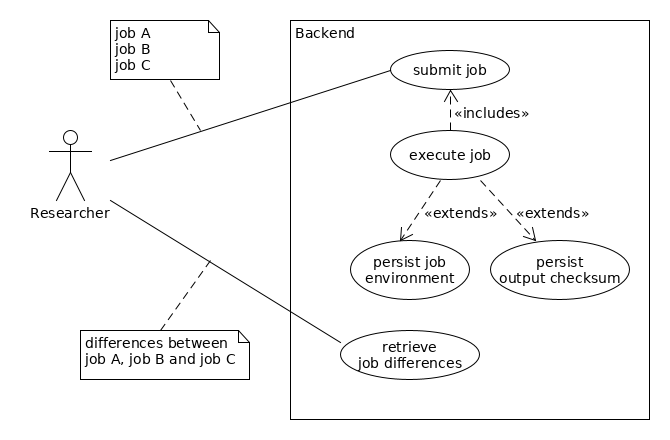
\includegraphics[width=\textwidth]{usecase3}
	\caption{Overview of the third use case: Compare different job executions}
	\label{fig:usecase3} % \label has to be placed AFTER \caption (or \subcaption) to produce correct cross-references.
\end{figure}
The third use case is dedicated to the comparison of job executions. The goal is for geoscientists to be able to compare different jobs not only by their results, but by the way they were executed. The same backend applies the comparison between a job execution and another job execution. Therefore, the processing implementation and the input data must be identifiable. To make the comparison more transparent to the users, additional data is added to the job environment data e.g. an output checksum. In addition to the previous conditions, a visualization of the differences for the users lowers the access barrier for them to use the feature. Figure \ref{fig:usecase3} gives an overview of this use case.
The following steps summarize the scenario sequence of actions: \\

\begin{itemize}
	\item \textbf{Job A}: Taking the minimum NDVI of the area of South Tyrol in May 2017. 
	\item \textbf{Job B}: Taking the minimum NDVI of the area of South Tyrol in May 2017.
	\item \textbf{Job C}: Taking the maximum NDVI of the area of South Tyrol in May 2017.
\end{itemize}

\begin{enumerate}
	\item Researcher runs a job (job A) at the backend.
	\item Researcher re-runs the same workflow used for job A at the same backend resulting in a new job (job B).
	\item Researcher runs a different job (job C).   
	\item Researcher receives a comparison of the jobs (A, B, C) by their environment and outcome.
\end{enumerate}



% Paper Problem continue





% Old Problem Description



% Old Motivation

%Over the last decades, remote sensing agencies have increased the variations of data processing and therefore, the amount of resulting data. The complexity of the experiments leads researchers to use external services for the workflow. These circumstances make it hard for scientists to provide the necessary information to enable reproducibility. Scientists create a description of the workflow and the used satellite identifier to describe experiments. It is necessary to have citable data and processes on the data to ensure long-term reproducibility to preserve the data for further usage in the future,  \cite{6352411}. 


%\section{Problem Description}\label{Problem}
%The vast majority of data used in earth observation sciences are retrieved and provided via \gls{soa} interfaces. Data providers like \gls{gee}\footnote{https://earthengine.google.com} and \gls{eodc}\footnote{https://www.eodc.eu} host a Web \gls{api} for data download and processing data. These services are used to define the experiment workflow, the definition of the input data, the execution, and the retrieval of the results. Therefore, the researcher is not in full control of the code execution and the environment of their experiments, since the information about the workflow environment of the experiment is not accessible for the scientists. Used external dependencies for processing the earth observation data cannot be accessed. The services act as black boxes to the researchers with no possibility to get versions of the used packages to calculate the resulting images. The situation leads to the problem that researchers are not capable of describing the experiments in a way that they are reproducible. \\
%Input data of a typical remote sensing workflow is satellite data of a specified satellite type filtered by a temporal and a spatial extent. The raw satellite data is preprocessed by the backend provider so that there is a global dataset. Geoscientists using the same satellite identifier could have different results after executing the same experiment if the provider updated the way the data is preprocessed. An example for this is the format update of \gls{esa} in 2017 of the Sentinel 1 dataset, which affected old data records, see \footnote{https://sentinel.esa.int/web/sentinel/missions/sentinel-1/news/-/article/sentinel-1-update-of-product-format}. When scientists use the dataset of a data provider, there is no possibility to see changes in the preprocessing algorithm. Therefore, data versions are not visible to the researcher. The situation leads to the problem that scientists are not capable of identifying the input data, which is a necessity for reproducibility.

%Due to a different range of functionality and a difference between the endpoints of the providers, it is great afford to create a workflow for more than one provider. The openEO project has the goal to be an abstraction layer above different EO data providers. Further information on the software architecture of the project is defined in the project proposal (\cite{openeo}) and in Section \ref{Related Work}. During the creation time of this thesis there is no consideration of repeatability in the openEO architecture. Verification of workflows for users of openEO is not in the agenda of the openEO project. Generalized layers have the opportunity to be implemented in a way that makes processes and data scientifically verifiable and reproducible, as it handles data and processes on the data in a standardized way for different providers. Even though the range of functionality and the API endpoints are well-defined in the openEO core-API, the contributing content providers (openEO backends) will have different underlying software execution environments. The used technology of an openEO backend will evolve in the future, hence it can lead to different results on the same workflow execution. Considering the following: A scientist runs an experiment using openEO as research tool and gets an arbitrary result. The same scientist runs the same experiment with the same input data some months later and gets a slightly different result. The question occurs, why are the results distinct? Has the used data changed, has the user accidentally submitted different code or has some underlying software inside the backend provider changed. Adding a possibility for the users of openEO to gain this information is an important feature for the scientific community. The aim of this thesis is to design an extension to openEO, so that users are able to retrieve provenance data about a job re-execution \cite{openeo}. 

%\section{Aim of the Work}\label{Aim}

\newpage
\section{Research Questions}\label{research question}\label{Aim}
The aim of the thesis is to propose a framework for making reproducibility conceivable in the earth observation community. The solution enables users to re-execute jobs and validate the results. It provides the scientists accessible differences in the execution of the job and the data, without changing their approach of doing research. To achieve this, a model for capturing the environment of the backends has to be discovered. Considering the problem description and the scenarios of the previous sections, the following research questions can be formulated:

\begin{itemize}
	\item \textbf{What information must be captured from an earth observation backend, so that a job execution can be repeated like the original execution?}
	\begin{itemize}
		\item How can the data of the original execution be identified?
		\item How can the environment of the original execution be reproduced?
		\item Which parts of the backend need to be extended?
		\item How can the result of a re-execution in future environments be verified?
	\end{itemize}
	\item \textbf{What information must be captured to enable validation of a job re-execution on an earth observation backend?}
	\begin{itemize}
		\item What are the validation requirements?
%		\item How can the data be compared?
	%	\item How can changes of input data at the backend be recognized?
		\item How can differences in the environment between the executions be discovered?
	\end{itemize}
\end{itemize}

The solution prototype is within \gls{openeo} (details see Section \ref{openEO}). It concludes with recommendations for the openEO specification on how to improve re-execution validation for the users. Using the standard of openEO enables to restrict the target of the thesis. It also facilitates all backends compliant to openEO an entrance to the proposed features of this thesis. 

\section{Methodological Approach}\label{Method}
There are already technologies available to solve parts of the issues described in the determined problem. This section provides the three key parts of the methodology used for the proposed solution of the thesis.

\begin{enumerate}
	\item \textbf{Data Identification}
	The input data has to be identifiable, to accomplish the capturing of jobs described in the use cases of Section \ref{Use Cases}. The \gls{rda} has identified 14 general rules \cite{rauber2016identification} for identification of data used in computation that allows to cite and retrieve the precise subset and version of data that existed at a certain point in time.
	
	\item \textbf{Job Environment}
	The VFramework \cite{MiksaBiomedical} and context model \cite{MayerOntology} were proposed to automatically document environments in which computational workflows execute and to enable their comparison. 
		
	\item \textbf{Backend Standardization}
	The openEO project \cite{openeo} works on creating a common EO interface to enable interoperability of EO backends by allowing researchers to run their experiments on different backends without reimplementing their code. We contribute to the openEO standard to provide compliant backends with reproducibility concepts.
	
\end{enumerate}

By combining these three elements, a scientific infrastructure is created that allows automatically documented and reproducible experiments to be executed with minimal overhead to the infrastructure and researchers performing their studies. We present this solution improving reproducibility of earth observation experiments executed at the openEO compliant backends. We follow the RDA recommendations for data identification and present how data provided by backends is made identifiable by assigning identifiers to subset queries made by researchers. We discuss which specific information must be captured, which interfaces must be modified, and which software components must be implemented. We also show how jobs executed at backends can be captured and compared using the VFramework to identify whether any differences in software dependencies among two executions exist.

\section{Structure of Work}\label{Structure}
This thesis is structured as follows. After this introduction, Chapter 2 gives an overview of related scientific activities in the area of reproducibility in the earth observation sciences and reproducibility in other areas with similar objectives. Chapter 3 provides the concept to address the research questions defined in Section \ref{research question}. It is the design used for the prototype implementation on the openEO compliant EODC backend described in the following chapter. Chapter 4 gives detailed insight into the modifications needed at the backend to achieve the features described by the use cases. The next chapter, Chapter 5 is concerned with the evaluation of the implementation of Chapter 4. For the evaluation we simulated typical use cases representing updates of data and changes in the backend environment. We also measured the performance and storage impact on the backend, which turned out to be minimal. 
Chapter 6 summarizes the outcome of the implementation and evaluation. It contains a discussion on results achieved and future work. 

\chapter{Related Work}\label{Related Work}


This chapter describes the related work that influenced this thesis. It informs the reader about concepts related to the proposed solution. The information is structured in subsections, each representing important technologies or concepts in the context of this thesis. \\The first section presents the concepts behind reproducibility in computer science. \\
The second section describes the state of reproducibility in earth observation science. \\
The third section presents concepts related to data identification. \\ 
The fourth section consists of other existing implementations to achieve reproducibility. \\
The last section of this chapter describes the openEO project and the EODC backend, which we use for the proof of concept implementation in Chapter \ref{Implementation}.      


\section{Reproducibility}\label{Reproducibility}
The term of reproducibility is defined as a new experiment based on an original experiment by an independent researcher in the manner of the original experiment. Reproducibility aims to gain additional evidence on the result of the original result by creating an independent experiment that shows similar results. Repetition defines a re-run of the same experiment with the same method, same environment, and a very similar result. The repetition aims to check if the methods described in a publication are resulting in the purposed outcome \cite{6064509}. 
Achieving reproducibility is a common problem in all scientific areas. Therefore there are ten rules defined to gain a common sense about reproducibility. They are motivated by the basic idea that every result of interest has to be associated with a used \gls{process} and data. The researcher has to provide external programs as well as custom script versions. Using version control software is recommended. Besides, one of the steps defines a rule to make scripts and their results publicly available \cite{10.1371/journal.pcbi.1003285}. 
Reproducibility is the crucial topic of The Fourth Paradigm. It leads to the term eScience, which has the aim of bringing science and computer technologies closer together. The general concept is to enable scientific procedures with new information technologies used by data-intensive sciences. The expected result of eScience is to get all scientific papers publicly available, including the necessary data and workflows, so that scientists can interact more efficiently \cite{noauthororeditorfourth}. 
eScience has the potential to enable a boost in scientific discovery. It provides approaches to make digital data and workflows citable. The publication \cite{Rauber2015RepeatabilityAR} discusses a general way of reaching this. It describes an approach to look at whole research processes by introducing Process Management Plans, other than limiting it to data citation. It demonstrates the capturing, verification, and validation of the input data for a computational process.
Computer sciences have the issue of high amounts of published papers that do not provide enough information to make them reproducible. This is not solved by the scientists that need to make additional effort, but by providing new tools for scientists that allow it automatically  \cite{MIKSA201725}. There are some additional issues on reproducibility in computer science e.g. in the case that used software technologies are deprecated and not available anymore. Therefore, persisting the execution context is needed to achieve a re-execution of the experiment. One proposed solution is the VFramework described in more detail in Section \ref{vframework}. 
The PRIMAD model defines a set of variables that define an experiment. The relationship of the original execution to a re-execution is visualized by noticing changes in the variables. The following variables of an experiment are used to describe the relationship \cite{primad}:

\begin{itemize}
	\item \textbf{P} Platform / Execution Environment / Context (e.g. Python 2.7, Windows 10,\dots) \\
	\item \textbf{R} Research Objectives / Goals (e.g. sorting the input) \\
	\item \textbf{I} Implementation / Code / Source-Code (e.g. script in Python) \\
	\item \textbf{M} Methods / Algorithms (e.g. quick sort) \\
	\item \textbf{A} Actors / Persons (e.g. researcher that is executing the experiment) \\
	\item \textbf{D} Data (input data and parameter values)   (e.g. input data that is to be sorted) 
\end{itemize}

If there is a re-execution that is different on every variable to the original one, except for the same method (M) and goal (R), it is considered a reproduction \cite{primad}. 
\\  
Data citation is a vital issue of reproducing results of past experiments. Preserving the exact workflow without persisting the original data has no positive effect on the scientific community. If the data used in an experiment is not available anymore, or not specified explicit enough, then there is no chance of reproducing it no matter how much information about the execution is known. In earth observation persisting the data for reproducibility in the future is an issue discussed in the literature \cite{6352411}. Gaining data identification in digital sciences has an official working group named \gls{wgdc}, which created 14 recommendations on data citation further explained in Section \ref{Data Identification}.

 \subsection{PROV-O}\label{PROV}
In 2003 the World Wide Web Consortium published the PROV model as a standard concerning provenance definitions. It is defined in twelve documents. In the context of this thesis the PROV Ontology (PROV-O) is the most relevant \cite{733f89c65e4844f9aabcae1c276a5602}. 
PROV-O is a standard language using OWL2 Web Ontology. It is a lightweight concept capable of a broad spectrum of applications.  

\begin{figure}[h]
	\centering
	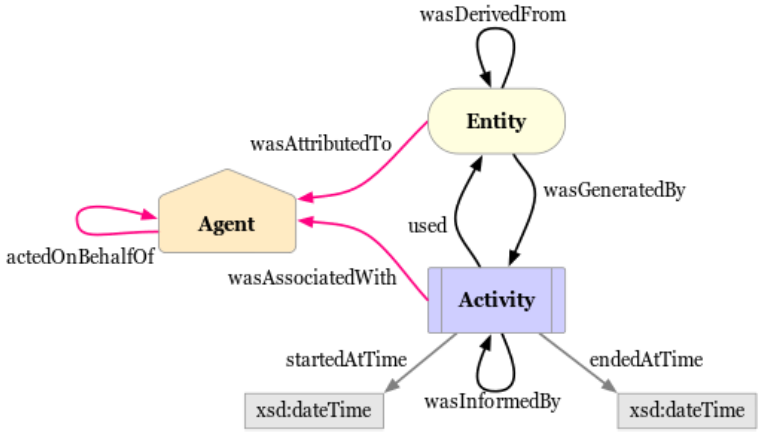
\includegraphics[scale=0.6]{prov}
	\caption{Overview of the main components of PROV-O \cite{733f89c65e4844f9aabcae1c276a5602}}
	\label{fig:prov} % \label has to be placed AFTER \caption (or \subcaption) to produce correct cross-references.
\end{figure}

Figure \ref{fig:prov} shows the basic setup of the PROV-O concept. It consists of three main elements. The \textit{Entity} is any physical, digital or conceptual thing. Provenance records describe \textit{Entities} that can consist of references to other \textit{Entities}. Another element is the \textit{Agent}, which is responsible for \textit{Activities} and that they are taking place, e.g. software, persons, or organizations. The association of an \textit{Agent} to an \textit{Activity} defines the responsibility of the \textit{Agent} for the \textit{Activity}. An \textit{Activity} describes what happened that the \textit{Entity} has come to existence and how attributes of an \textit{Entity} changed \cite{733f89c65e4844f9aabcae1c276a5602}. The design chapter \ref{Design} does not specify the representation of the context information. Therefore the PROV ontology can be used to represent the information. \bgoesswein{This thesis implements the PROV-O standard as one of the available provenance representations for the user. Section \ref{Implementation:PROV-O} shows how we implemented it.}
%since the EODC backend providers wanted their representation of it, which is an extension of the existing data representation, but it is a reasonable extension. 
%\todo{Design Decision EODC analysieren --> anderes Chapter aber hier verlinken...}
\subsection{VFramework}\label{vframework}

The VFramework defines parallel capturing of provenance data during the workflow execution. During the original execution, evidence gets collected into a repository e.g. logging. The context model of the execution persists the needed data e.g. in a database record. Re-execution is verified and validated using the provided provenance data in the context model of the original execution and the context model of the re-execution. The provenance data divides into static and dynamic data. Static data defines data that is not dependent on the execution of the experiment e.g. the operating system and installed packages. The static environment information is, therefore, independent of the configuration of the workflow. Dynamic data is captured during the execution of the original experiment e.g. Python version of the execution or used input files. It describes data dependent to a workflow execution \cite{Miksa2013FrameworkFV}. 
Figure \ref{fig:vframework} shows an overview of the VFramework concept described above.   
\begin{figure}[h]
	\centering
	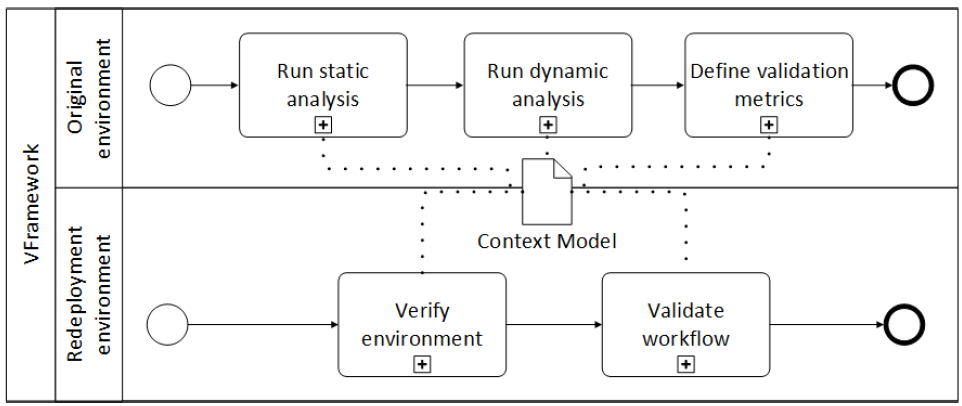
\includegraphics[width=\textwidth]{vframework}
	\caption{Overview of the Concept of the VFramework \cite{Miksa2013FrameworkFV}}
	\label{fig:vframework} % \label has to be placed AFTER \caption (or \subcaption) to produce correct cross-references.
\end{figure}

\section{Earth Observation Science}\label{EOScience}

This section describes Reproducibility in the context of the computational geoscience. A study tests the reproducibility and replicability of scientific papers in geoscience by obtaining more than 400 papers \cite{Ostermann2017AdvancingSW}. In \cite{Ostermann2017AdvancingSW} a reproduction is defined by an exact duplicate of an experiment, whereas it defines replication as a resemblance of the original execution, but allowing variation e.g. different scales. Table \ref{Tab:geoprimad} describes the difference between reproduction and replicability in PRIMAD terms. Since the definition of the paper differs from the definition of this thesis the terms are marked as Reproducibility' and Replicability'. Only half of the test group publications are replicable, and none of them reproducible. There are publications to address the lack of reproducibility in the earth observation science. The following sections summarize these concepts.     

\begin{table}[]
	\caption{PRIMAD description of reproduction and replication according to \cite{Ostermann2017AdvancingSW}}
	\begin{tabular}{l|l|l}
		 & \textbf{Reproduction'} & \textbf{Replication'}  \\ \hline
		\textbf{P}latform & same & different \\ \hline 
		\textbf{R}esearch Objectives & same & same \\ \hline  
		\textbf{I}mplementation  & same & different  \\ \hline  
		\textbf{M}ethods & same & different \\ \hline 
		\textbf{A}ctors & different & different \\ \hline
		\textbf{D}ata & same & different, but similiar \\ \hline
	\end{tabular}
	\label{Tab:geoprimad}
\end{table}

\subsection{Vadose Zone Journal (VZJ)}\label{VZJ}
In order to face the issue of reproducibility in geoscience the \gls{vzj} started a \gls{rr} program in 2015 \cite{doi:10.2136/vzj2015.06.0088}. 
The earth observation science is a big part of VZJ publications, and most of them are not applying the open computational science guidelines. The main reasons are behaviors of scientists that do not see the overall benefit of putting effort into documentation. Therefore, the VZJ started an RR program to publish the code and data alongside scientific papers. The aim of the strategy is to lower the access barrier for scientists to publish their research work entirely. Goal of the project is to create a community of researchers with a shared sense of reproducibility and data citation on the platform. The community then animates other scientists to join the approach. On time this thesis is written, the service is still available\footnote{https://dl.sciencesocieties.org/publications/vzj/author-instructions-reproducible-research}, but there were no results available on how much it is used \cite{doi:10.2136/vzj2015.06.0088}.

\subsection{The Geoscience Paper of the Future (GPF)}\label{GPF}

Geoscience Papers of the Future (GPF) \cite{Gil2016TowardTG}  is an initiative to encourage geoscientists to publish papers together with the associated digital products of their research. This means that a paper would include: 

\begin{enumerate}
	\item documentation of datasets, including descriptions, unique identifiers, and availability in public repositories; 
	\item documentation of software, including pre-processing of data and visualization steps, described with data and with unique identifiers and pointers to public code repositories; 
	\item documentation of the provenance and workflow for each figure or result.
\end{enumerate}

\begin{figure}[h]
	\centering
	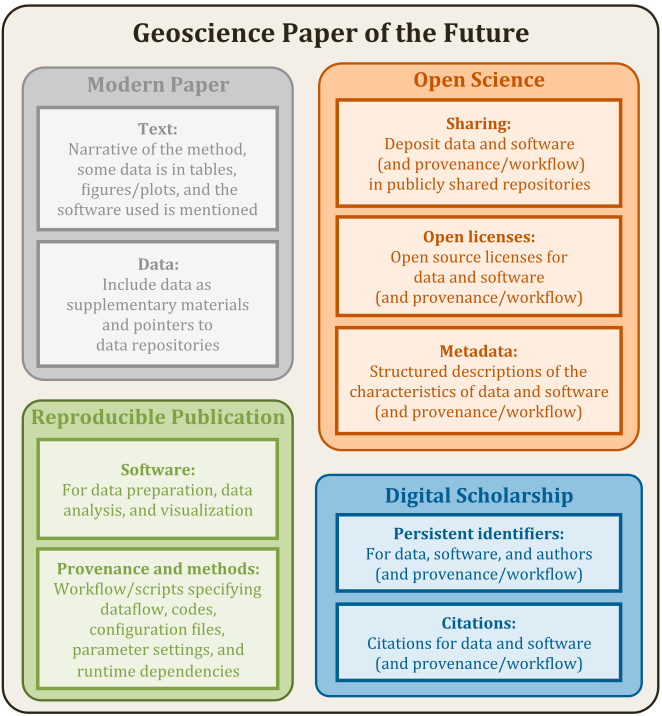
\includegraphics[scale=0.5]{gpf}
	\caption{Relationship between reproducible publications and geoscientific papers of the future \cite{Gil2016TowardTG}}
	\label{fig:gpf} % \label has to be placed AFTER \caption (or \subcaption) to produce correct cross-references.
\end{figure}

Figure \ref{fig:gpf} visualizes the differences with a reproducible paper. In addition to the characteristics of the reproducible paper, the GPF focuses on publishing the data publicly with open licenses with citable persistent identifiers.
The GPF proposes a set of 20 recommendations for geoscientists regarding data accessibility, software accessibility, and provenance information. GPF authors may have reasons to be not able to follow all rules and therefore, have to find workarounds and propose areas for future improvements. The strategy of the GPF community is to educate the scientist to make reproducible publications, by making training sessions\footnote{http://scientificpaperofthefuture.org/gpf/events.html}, instead than providing tools. The solution of this thesis aids in providing information requested above by precisely identifying datasets and software (including version and libraries) used by backends to compute results. This information is collected automatically and can be accessed by users any time using the same API as they use for implementation of their experiments.  

\subsection{Climate Change Centre Austria (CCCA)}

The \gls{ccca} is a research network for Austrian climate research available since 2016. Its aim is the provision of climate-relevant information, the inter-operable interfaces, and long term archiving of scientific data. In 2017, data citation for the \gls{netcdf} format was added to the project. The architecture of the implementation and the technology used in the background is similar to the set up of the EODC backend. Therefore, the approach of enabling data identification was similar to this thesis. CCCA is open source and available at GitHub\footnote{https://github.com/ccca-dc}. Similar to the approach of this thesis, the concept for data identification are the RDA recommendations. Figure \ref{fig:ccca} shows a technical overview of the CCCA implementation. It uses a ckan\footnote{https://ckan.org} web server to handle the request and responses of the user, which are then passed to a Python application. The Python application is responsible for the query store functionality. The core element is the \gls{tds}\footnote{https://www.unidata.ucar.edu/software/thredds/current/tds/}, which is responsible for the data archiving.   
The Python application of the CCCA overview is similar to the implementation of this thesis. The main difference is the objectives of the CCCA service compared to the EODC backend. On the CCCA platform, any climate-relevant information (e.g. air temperature or frost days) can be uploaded and persisted. On the EODC backend, preprocessed global earth observation data is persisted, which is used as input data for processing chains. Therefore, the data on EODC is more homogeneous than the data on the CCCA platform.
Nevertheless, the concept of enabling data identification is similar in both projects. The CCCA implementation inspired the query store implementation of this thesis. The query result differs, because EODC uses a different file format (\gls{geotiff} instead of NetCDF). Another difference is that CCCA uses HTTP GET requests as query, whereas the EODC backend uses \gls{xml} based queries, which are restricted by the openEO API specification \cite{ccca}.  

\begin{figure}[h]
	\centering
	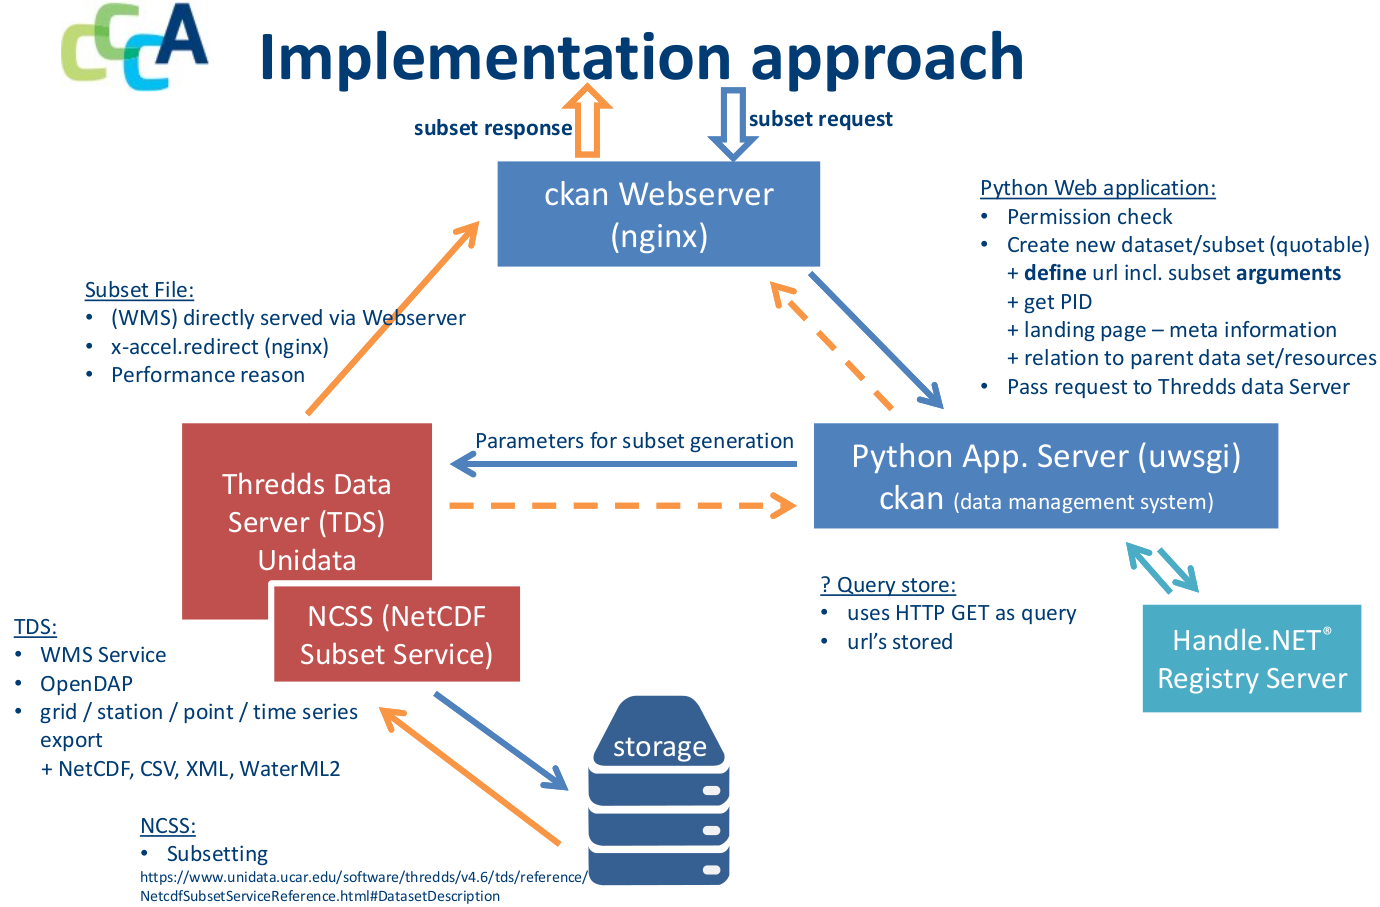
\includegraphics[scale=0.25]{ccca}
	\caption{Technical overview of the CCCA NetCDF data citation implementation}
	\label{fig:ccca} % \label has to be placed AFTER \caption (or \subcaption) to produce %correct cross-references.
\end{figure}

\section{Data Identification}\label{Data Identification}

For the aim of this work, the input data is a key element of the captured data. If the input data can not be identified correctly, the capturing of the processing on it does not gain useful information. Therefore the identity of the data has to be guaranteed. The Research Data Alliance (RDA)\footnote{https://rd-alliance.org} is an international body issuing recommendations helping to remove barriers in data sharing. Recommendations are based on a community consensus worked out within working groups. The Data Citation working group\footnote{https://rd-alliance.org/groups/data-citation-wg.html} has identified 14 rules for identification of data used in computation. It allows to  identify and cite arbitrary views of data, from a single record to an entire data set in a precise, machine-actionable manner. Further it enables to cite and retrieve that data as it existed at a certain point in time, whether the database is static or dynamic. In the following the recommendations are summarized \cite{rauber2016identification}:

\begin{itemize}
	\item \textbf{R1: Data Versioning} \\
	Changes on a data record must result in a new version of the data record and the persistence of the deprecated data records. All data record versions have to be identifiable and accessible. 
	\item \textbf{R2: Timestamping} \\
	All changes to the database have to be comprehensible via timestamps. Every time changes are applied to the data, there has to be a timestamp persisted to describe when it happened. 
	\item \textbf{R3: Query Store Facilities} \\
	There has to be a query store implemented at the data provider. The applications uses it to store queries and additional information. The database has to store, according to \cite{rauber2016identification}, the following things: 
	\begin{itemize}
		\item The original query as applied to the database
		\item A potentially re-written unique query created by the system (R4, R5)
		\item Hash of the (unique) query to detect duplicate queries (R4)
		\item Hash of the result set (R6)
		\item Query execution timestamp (R7)
		\item Persistent identifier of the data source
		\item Persistent identifier for the query (R8)
		\item Additional information (e.g. author or creator information) required by the landing page (R11)
	\end{itemize}
	\item \textbf{R4: Query Uniqueness} \\
	Since it is not desirable to have equal queries with the same result stored at the query store, there needs to be a unique query that can be directly compared to other queries. Hence, there needs to be an algorithm to normalize the queries and to guarantee their uniqueness.
	\item \textbf{R5: Stable Sorting} \\
	The sorting of the resulting data has to be unambiguous, if the sequence of data item presentation is essential for the reproduction.
	\item \textbf{R6: Result Set Verification} \\
	To ensure that the resulting data of the query is comparable there have to be a checksum or hash key of it. 
	\item \textbf{R7: Query Timestamping} \\
	There has to be a timestamp assigned to every query in the query store, which can be set to the latest update of the entire database, or the query dependent data of the database, or simply the time of query execution.
	\item \textbf{R8: Query PID}\\
	Every query record in the query store must have a Persistent Identifier (PID). There must not be a query with the same normalized query and query result checksum tuple. 
	\item \textbf{R9: Store the Query} \\
	The data described in previous recommendations have to be persisted in the query store.
	\item \textbf{R10: Automated Citation Texts} \\
	To make the citation of the data more convenient for researchers, there shall be a automatic generation of the citation text snipped containing the data PID.
	\item \textbf{R11: Landing Page} \\
	The PID shall be resolvable in a human readable landing page, where data mentioned in the previous recommendations is provided to the scientist.
	\item \textbf{R12: Machine Actionability} \\
	Providing an API landing page so that not only humans, but machines can access the data by resolving the PID.
	\item \textbf{R13: Technology Migration} \\
	If the query store needs to be migrated to a new system, the queries have to be transferred too. In addition the queries have to be updated according to the new setup, so that they still work exactly like in the old system.
	\item \textbf{R14: Migration Verification} \\
	There shall be a service to verify a data and query migration (see R13) automatically, to prove that the queries in the query store are still correct. 
\end{itemize}

The recommendations provide a generic set of rules independent of an application domain. So far they have been implemented in settings ranging from atomic and molecular data \cite{data_atomic}, climate change \cite{Schubert} to health policy planning \cite{data_health}. We use them also in our solution to make data provided by backends identifiable, by assigning PIDs to queries identifying the subsest of data selected by researchers for their analyses.

\section{Tools for Reproducibility}\label{Existing Tools}
The section describes tools that are designed to solve similar problems or subproblems addressed by this thesis. There is an explanation of why the specific tool was not used for the prototype of this thesis or how it was used in parts of the solution. 

\subsection{noWorkflow}\label{Noworkflow}
noWorkflow is introduced in 2015 as a provenance capturing tool with the aim of not influencing the way researchers work. As proof of concept, noWorkflow uses Python as programming language. A SQLite database stores the provenance information categorized in trials. A trial represents the environment information of one execution. The main benefit of noWorkflow is that it does not instrument the code, and it automatically captures the definition, deployment, and execution environment in a local SQLite database. The command line interface of noWorkflow is capable of providing access to the stored data. In addition to just retrieving the information about the execution environment, analyses features are added Figure \ref{fig:noworkflow} gives an overview of the noWorkflow architecture. It shows the three modules of capturing, storing and analyzing of the provenance data \cite{c9e0604becba42af96a9cb0a6f60018b}.

\begin{figure}[h]
	\centering
	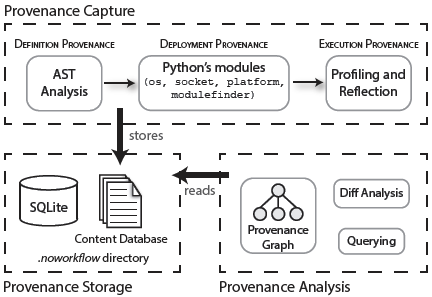
\includegraphics[scale=1]{noworkflow}
	\caption{Architecture of noWorkflow \cite{c9e0604becba42af96a9cb0a6f60018b}}
	\label{fig:noworkflow} % \label has to be placed AFTER \caption (or \subcaption) to produce correct cross-references.
\end{figure}

The noWorkflow framework improved regularly after the first announcement. noWorkflow was extended by an feature of tracking the evolution of the trials \cite{Pimentel2016TrackingAA}. It improves the possibility to compare trials and to visualize the history of past trials. Next, the fine-grained provenance tracking extension of noWorkflow is introduced \cite{Pimentel:2016:FPC:3090188.3090214}. It enables to split the trial into single execution lines. It adds a visualization of all called functions in a graph. It has the limitation of multiple function calls in one line on complex data structures such as dictionaries, lists, and objects. Next, noWorkflow combines with yesWorkflow, the concept of gathering information about the provenance using comments and annotations \cite{192094}. The combination enabled more detailed environment information, querying, and visualizations \cite{69bac1252a684629baa43b48e350068d}. 
In this thesis, noWorkflow was used in an early attempt for the implementation but is not part of the final solution due to the high amount of the captured data by noWorkflow and the additional requirements needed by the EODC backend for using it.

\subsection{ReproZip}\label{ReproZip}
ReproZip is a packaging tool to enable the reproducibility of computational executions of any kind. It automatically tracks the dependencies of an experiment and stores it into a package. ReproZip can execute the package on another machine. Additionally it is capable of letting the re-executor modify the original experiment. It was developed for the SIGMOD Reproducibility Review\footnote{http://db-reproducibility.seas.harvard.edu/}. Figure \ref{fig:reprozip} shows the architecture of ReproZip. ReproZip traces the system calls to create a package configured by the configuration file. Thus, it produces a single file with the extension “.rpz”. ReproZip opens these files, unpack them and re-executes it on a different machine. ReproZip aims to make reproducible science easy to apply for single experiments \cite{29c5846926a4497d95f276604cb0368c}. The reason why it is not used in the solution of this thesis is that the capturing is very fine granulated. This takes too much performance from the backends, which is a key selling point for backend providers. Depending on the backend, the payment for users may be dependent on the duration time of the processing. Another issue with ReproZip in the context of this thesis is that it is not capable of capturing the big data of the backends within the package, because it would take too much space and performance.   

\begin{figure}[h]
	\centering
	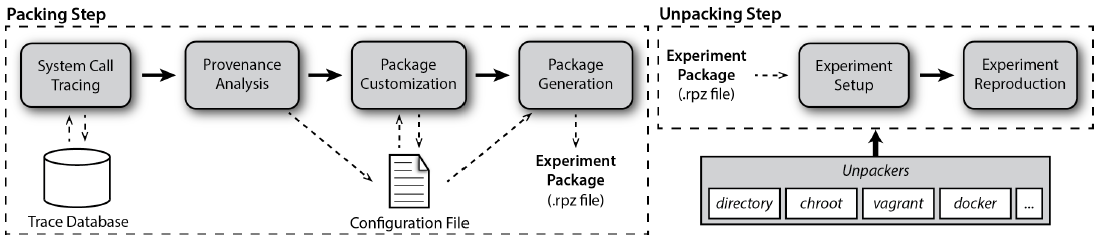
\includegraphics[width=\textwidth]{reprozip}
	\caption{Overview of the ReproZip concept from \cite{29c5846926a4497d95f276604cb0368c} }
	\label{fig:reprozip} % \label has to be placed AFTER \caption (or \subcaption) to produce correct cross-references.
\end{figure}

\subsection{Docker / Smartcontainer}\label{Smartcontainer}
Docker containers are ubiquitous in geoscience executions. The advantages of reproducible research and cost savings by using Docker containers are discussed in the community for the \gls{geobia} \cite{rs9030290}. The implementation of the image analysis is implemented with a docker image with a user interface that can also be used by non-experts. Studies for the more general \gls{obia} using this Docker containers were carried out \cite{proceedings456}. The conclusion is definite, with only little shortcomings in the usability. The aim was to use docker images to make it easier for scientists to re-run an experiment on the OBIA system. The remaining question is how the docker configuration is preserved in a manner that it can be reproduced within different environments. Therefore, a "workflow record" is introduced by storing the environment and entities involved in addition to the Docker description file. SPARQL query is introduced to create the possibility to use the container as a repository of data \cite{emsley2017a}.\\ 
Smart container is another approach of preserving a docker container. The aim of a smart container is an ontology and software to preserve docker data. It uses the PROV-O standard to define the provenance \cite{Huo2015SmartCA}. 
Docker containers are used at the EODC backend for running all services. Therefore they are part of the solution. The description files of the used docker containers are persisted in the GitHub repository of the EODC backend. Hence they are identifiable by the backend version defined in Section \ref{Design}.   

\subsection{Version Control Systems}\label{Version Control Systems}
\gls{vcs} became an essential part of all computational sciences. It enables to persist versions of code and the possibility to head back to a particular version. Before that, programmers tend to have multiple directories to make versions of the code. The basic idea of VCS is a command line interface that makes it possible to set a version of the current state of the code. These versions can be accessed in the future, without changing other versions of the code and without manually added folder structures \cite{10.1109/MCSE.2009.194}. 
In this thesis, we use Gitorious (Git) as VCS of the solution. Versions in Git are defined as commits and are stored locally and can be published to an external server. There, other users can access the commits if they have enough rights set. The commits are stored both, locally and remotely \cite{QuickGit}. openEO uses Git as default code versioning tool. GitHub is used as the publicly available server. Since openEO is an open source project, the code of every backend, core API and the client software is available at GitHub without restrictions. 

\subsection{Hash}\label{Hash}
Hash functions are used to validate data without having to save the whole data. They have two
important properties to work correctly. First, the probability that two different inputs have the same hash outcome has to be low. Second, it must to be hard to find a message with the same hash value as an already known message. These properties makes the hash functionality a standard tool to identify data without having to save the original \cite{3b412889270f46f59740fbf1ca8cd7e0}.  
In this thesis, the \gls{sha}-256 is used for the entries of the context model, mostly to compare differences in data outcomes.

%\begin{figure}[h]
%	\centering
%	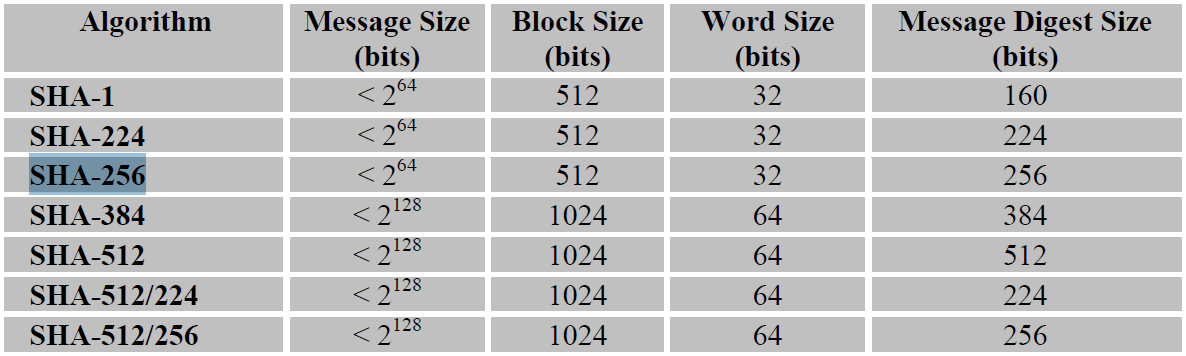
\includegraphics[width=\textwidth]{sha}
%	\caption{\cite{shapaper}}
%	\label{fig:sha} % \label has to be placed AFTER \caption (or %\subcaption) to produce correct cross-references.
%\end{figure}
%The SHA-256 is chosen in the implementation, because of the best combination of performance and security of the above described properties of the hash. 

\section{openEO}\label{openEO}
The openEO project consists of three modules. The client module written in the programming language of the users and entry point of the users. Second, the backend drivers that enables for every backend to understand the calls from the clients, so the interface at the backends to support openEO. Third, the core API, which specifies the communication. The core API is the key element of the openEO project and a standard that the backend providers accepted to implement on their systems to be openEO compliant. The backend drivers are the translation of the client calls to the backends specific APIs. This architecture decouples the clients from the backends so that every openEO client can connect to every openEO compliant backend. An example of a workflow is the example defined in Section \ref{example} using the Python client to access the openEO interface of the EODC backend \cite{openeo}. 

The communication is specified as an OpenAPI description, which is a way of defining \gls{rest}ful communication in a standardized way. The definition consists of the endpoints at the backend and the requests and the responses. The whole communication protocol is specified with OpenAPI \cite{openapi}. 
In the following, the relevant RESTful request types in openEO and the policy of choosing between them are introduced:

\begin{itemize}
	\item \textbf{GET Request} \\
	GET requests are used to retrieve data \bgoessweindel{and data} from the backends. The functionality is limited to read operations. \\(e.g. GET /collections returns a list of available collections at the backend.)
	\item \textbf{POST Request} \\ 
	POST requests are used to create \bgoessweindel{data and} new data records at the backend. It is also used to send information in the body of the request. \\(e.g. POST /jobs creates a new processing job at the backend, which is defined in the body of the request. It creates a new job identifier.)  
	\item \textbf{PATCH Request} \\
	PATCH requests are used to update existing records at the backend. \\(e.g. /PATCH /job/{job\_id} modifies an existing job at the backend but maintains the job identifier.)
	\item \textbf{DELETE Request} \\ 
	DELETE requests are used to remove existing records at the backend. \\(e.g. /DELETE /job/{job\_id} removes an existing job from the backend.)
\end{itemize}

\begin{figure}[h]
	\centering
	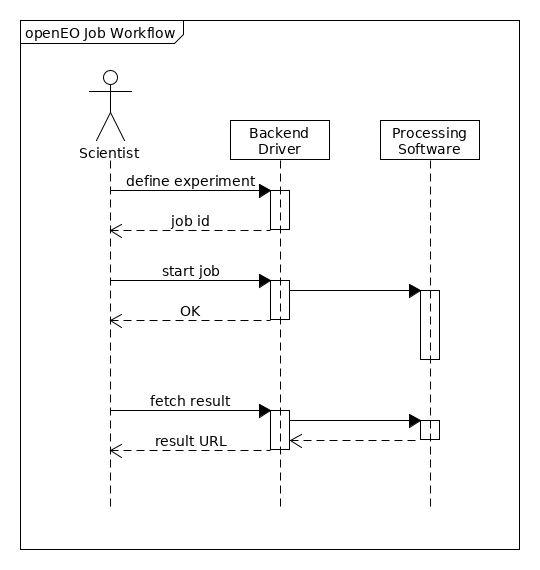
\includegraphics[scale=0.5]{sequence_diagramm2}
	\caption{Overview of the openEO procedure to execute a job and retrieve the results}
	\label{fig:api2} % \label has to be placed AFTER \caption (or \subcaption) to produce correct cross-references.
\end{figure}


\subsection{Job Execution}\label{Job Execution}
Figure \ref{fig:api2} shows a sequence diagram of a job execution using the client application and an openEO compliant backend. Users define the workflow in a client-specific programming language using the openEO client. The main parts of the job execution definition is the description of the input data, the filter operations and the processes that should be executed on the filtered data. Therefore, openEO introduces the \gls{processgraph}. openEO defines it as a tree structure of processes with their input data and successor process. The openEO coreAPI specifies every operation as process, even filter and data retrieval operations. The process graph is in \gls{json} format and gets generated by the clients in the background without users having to deal with it directly. Figure \ref{fig:process_graph} shows the running example process graph defined in Section \ref{example}.  

\begin{figure}[h]
	\centering
	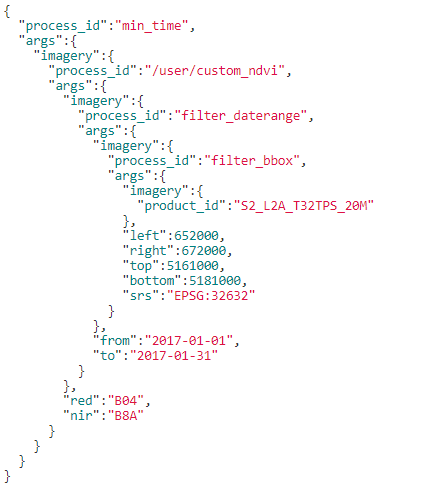
\includegraphics[scale=1]{process_graph}
	\caption{Process graph of the running example defined in Section \ref{example}}
	\label{fig:process_graph} % \label has to be placed AFTER \caption (or \subcaption) to produce correct cross-references.
\end{figure}


The backends interpret the process graph from inside out. Figure \ref{fig:process_graph} displays the process graph of the running example of Section \ref{example}. It describes the calculation of the minimum NDVI image of the Sentinel 2 satellite over South Tyrol in May 2017. The element in the center of the process graph defines the input data identifier in the "imagery" block, with the "get\_collection" process id. In this case, "s2a\_prd\_msil1c" is chosen as input data identifier, since it defines Sentinel 2 data at the EODC backend.
After reading the input data id, the backend iterates one step up in the hierarchy of the process graph and calls the process "filter\_bbox" with the parameters "west", "east" etc.. It filters the satellite data spatially, by only considering data within the bounding box (e.g. the area over South Tyrol). Next, the "filter\_daterange" process is used to filter the imageries temporally, by only using data from May 2017. Every process beginning with "filter\_" is defined as filter process, so an operation that restricts the input data. 
\bgoesswein{How the filter operations are implemented depends on the infrastructure of the backend provider. Section \ref{EODC Back End} shows how EODC implements it.}
The output data of the previous process is the input data of the next process. After the last filtering process, the NDVI gets called by the process "NDVI" with the parameters "red" and "nir". They are setting the identifier of the bands of near-infrared and red light used by the backend. The two bands are used in the formula of the NDVI calculation (see Section \ref{example}). Next, the minimum value is taken from all images using the "min\_time" process. It is a reducer process, which transforms the image stack of May 2017 into a single result image. Figure \ref{fig:process_graph_diagram} shows the same process graph from the backend point of view. It visualizes the order of how the processes are executed. To transmit the process graph of Figure \ref{fig:process_graph} at a backend, the openEO client puts it into the body of the POST /jobs endpoint request.
%\todo{you should add a short description of how this filtering process works in OpenEO / EODC. This will be needed later-on when you discuss the versioning, and when yoh show that, after an update to the DB, the same query produces a different list of filenames, but that you can also re-run an old query, still producing the same list of filenames. This is a key element in the process! You can do this here kr.point to Sec 2.5.3 when yoh dis uss the backend, the Postgres and GIS plugin.}
\begin{figure}[h]
	\centering
	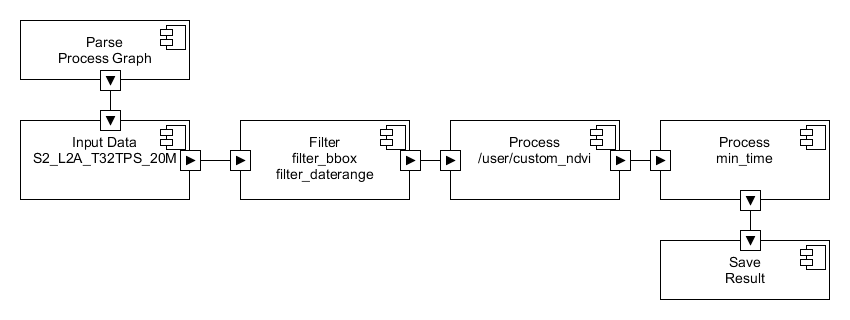
\includegraphics[width=\textwidth]{backend_pg}
	\caption{Action chain of the backend after receiving the process graph of Figure \ref{fig:process_graph}}
	\label{fig:process_graph_diagram} % \label has to be placed AFTER \caption (or \subcaption) to produce correct cross-references.
\end{figure}

There are two different kind of process executions depending on the capabilities of the backend named synchronous and asynchronous calls. Synchronous calls are directly executed after the backend receives them, and the script of the user has to wait until the job is finished for proceeding. For example, the program waits after sending the process graph to the backend until the backend returns the result. An asynchronous call does not get executed until the user starts the execution on the backend through an additional endpoint call. When the processing is finished, the user can download the result at another endpoint of the backend. For asynchronous calls, there is the possibility to subscribe to a notification system on the backend, so that the user gets notified when the job execution finished.     
The processes are defined at the openEO core API and independent of the backend they get called at, other than the data identifier, which may differ at each backend.  
\\
The previous example uses a process graph that only consists of the available processes and data of the backend. Within the openEO\footnote{https://github.com/Open-EO/openeo-openshift-driver/tree/release-0.0.2} project, there is the possibility to define individual processes and execute them on the backend. In the project, they are called “user defined functions” and are at the writing of this thesis still not well-defined. The plan is to send code written by the openEO user to the backend and execute it there in a secure virtual environment. The user can define processes and can run them with the data provided at the backend, using the infrastructure of the backend. Every backend has to define what the restrictions on user defined functions are. 

\subsection{Backends Overview}\label{Backend Overview}
Even though the backends implement the openEO core API standard, they are still diverse behind this abstraction layer. Most backends have already an API, where the openEO calls are translated to. There are 7 partners within the openEO project that are implementing a backend driver. The backends have to implement a translation of the process graph to the internal system. The billing of the users can be completely different on every backend. Table \ref{Tab:backends} gives an overview of all contributing openEO backends and their related GitHub repository.
\begin{table}[]
	\caption{List of all backend providers of the openEO project}
	\begin{tabular}{l|l}
		\textbf{Organisation} & \textbf{GitHub}  \\ \hline
		EODC & \url{https://github.com/Open-EO/openeo-openshift-driver} \\ \hline 
		VITO & \url{https://github.com/Open-EO/openeo-geopyspark-driver} \\ \hline  
		Google  & \url{https://github.com/Open-EO/openeo-earthengine-driver} \\ \hline  
		Mundialis & \url{https://github.com/Open-EO/openeo-grassgis-driver} \\ \hline 
		JRC & \url{https://github.com/Open-EO/openeo-jeodpp-driver} \\ \hline
		WWU & \url{https://github.com/Open-EO/openeo-r-backend} \\ \hline
		Sinergise & \url{https://github.com/Open-EO/openeo-sentinelhub-driver} \\ \hline
		EURAC & \url{https://github.com/Open-EO/openeo-wcps-driver} \\ 
	\end{tabular}
	\label{Tab:backends}
\end{table}

\subsection{EODC Backend}\label{EODC Back End}

The EODC backend is one of the contributing backend providers of the openEO project. The backend is implemented in Python and operates job executions with docker. EODC decided to use OpenShift (using Kubernetes) \footnote{https://www.openshift.com/learn/what-is-openshift/} to balance the workload of the docker container. It is capable of scaling docker containers and provides version control on them. The docker container execute the Python code for executing the processes. The docker description files and the Python code are available on GitHub. In this thesis, the latest version of the EODC backend provided in GitHub using openEO coreAPI version 0.3.1 is used. Every process of the openEO process graph is represented by an own Docker container. The Python library flask accomplishes the service layer for the RESTful API of the EODC backend driver. EODC provides only data from Sentinel 2 and Sentinel 1 within the openEO project. They are satellite images from Copernicus in cooperation of the European Space Agency (ESA), which receives the raw data directly from the Sentinel satellites. \\
The data management of EODC is file-based, so every image data is stored in a different directory and filename combination. The path of the file is the identifier of a data record. Data is provided via PostgreSQL database including the PostGIS\footnote{https://postgis.net} plug-in. \bgoesswein{In addition to the basic PostgreSQL functionality the plugin enables filtering by spatial and temporal extent. The datasets contain the bounding box coordinates and the timestamp of the capturing as well as a creation timestamp. It enables to query all datasets inside of a given area and timerange within SQL syntax. The plugin is capable of returning the most recent datasets in terms of creation timestamps, so that only one version of a dataset is returned. We use an additional "WHERE" clause to filter datasets that have a creation timestamp before a certain time. So that we can get the versions of datasets available at a given time.}The provided query tool for EODC users is the \gls{ogc} standard interface \gls{csw}\footnote{http://cite.opengeospatial.org/pub/cite/files/edu/cat/text/main.html}.\bgoesswein{It is used for the communication to the web interface of the EODC database.} Figure \ref{fig:eodceer} gives an overview of the EODC database structure. It is retrieved from the GitHub repository of the EODC backend\footnote{https://github.com/Open-EO/openeo-openshift-driver}, where every database entity is defined. A process entity can have parameters described by the parameter entity. The process node is representing one node in a process graph and is therefore related to exactly one process graph entity. Every job is related to a process graph. There may be jobs that use the same process graphs, but in the current set up they are persisted both separately in the database.

\begin{figure}[h]
	\centering
	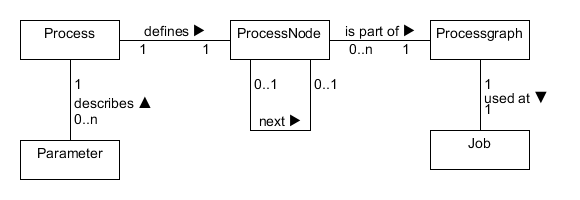
\includegraphics[width=\textwidth]{eodc_eer}
	\caption{Overview of the EODC database structure.}
	\label{fig:eodceer} % \label has to be placed AFTER \caption (or \subcaption) to produce correct cross-references.
\end{figure}

\section{Summary}

The research areas related to the solution of this thesis has a vast amount of available literature. The problem description of the thesis has many related existing solutions described in this chapter. The outcome of this thesis has the aim of making it easy for the scientists to reproduce experiments and therefore enable job re-execution at the backend. Other than presented solutions for earth observation science like the approach of VZJ and the GPF, which only provide informal support for scientists. The implementation of Section \ref{Implementation} builds on existing systems like the implementation of the CCCA query store, the RDA recommendations and the VFramework. The following chapter describes the design of the solution. 
 
\chapter{Design}\label{Design}


The core of this thesis is an extension design for EO backends providing users reproducibility. This chapter describes the proposed generic design that can also be applied to other similar domains. This chapter aims to present the design and is structured in six parts. The first part presents an overview of the design. The next three sections describe the main components in more detail. First,  the data identification component, then the component of capturing the provenance of the job execution. Third, the component for capturing and validation the result. The next section defines the resulting context model and its elements. The last two sections define the user services, suggestions on backend API extensions and \gls{udf}. The next Chapter \ref{Implementation}, shows an implementation of the outcome of this chapter at the EODC backend. 

\section{Overview}\label{Design:Overview}
This section gives an overview of the design. Figure \ref{fig:overview} shows an overview of the design. White boxes represent the components that every backend driver has already in place. The green elements in Figure \ref{fig:overview} are the proposed extensions to the backend. The following steps describe a typical job execution workflow for a better understanding of the backend functionality:

\begin{figure}[h]
	\centering
	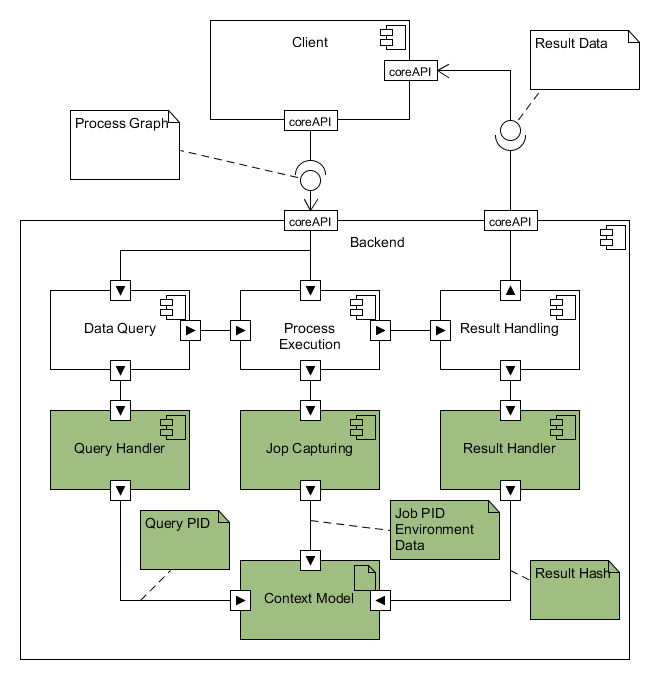
\includegraphics[scale=0.6]{design_overview_paper}
	\caption{Overview of the design}
	\label{fig:overview} 
\end{figure}


 \begin{enumerate}
	\item \textbf{\gls{eo} Client} \\
	The user defines input data, filter operations, and processes, which define the workflow of an experiment, via an EO client. After that, the user orders with the client the creation of a new job at the backend. Therefore, the client creates a process graph description and sends it to the backend. The client application is used to start the execution of the job and to receive the results. The following steps describe the backend internal procedures after starting the execution of a job.
	\item \textbf{Data Query} \\ 
	The \textit{Data Query} component receives the process graph and parses the data identifier and the filter operations. They are used to build a internal query to select the input data required by the job execution. \textit{Data Query} forwards the resulting data of the query execution to the \textit{Process Execution} component.
	\item \textbf{Process Execution} \\
	The \textit{Process Execution} component receives the process graph and the input data from the \textit{Data Query} component. It parses the processes from the process graph and executes them in the order of appearance. After every process executed, the \textit{Process Execution} component forwards the resulting data to the \textit{Result Handling} component.   
	\item \textbf{Result Handling} \\ 
	The \textit{Result Handling} component receives the results from the \textit{Process Execution} component and stores all job related meta data and the result. If ordered by the client application, the \textit{Result Handling} sends a link to the output files back to the client. In addition does the \textit{Result Handling} component provide meta data of the job execution to the user via the client. 
\end{enumerate}

The design of this thesis aims to make all three backend internal components identifiable. This enables to make the whole job execution reproducible. Hence, we introduce the following elements as additional components to the backend.

 \begin{itemize}
	\item \textbf{Query Handler} \\
	The \textit{Query Handler} component applies data identification to the backend. It does so by applying the RDA recommendations described in Section \ref{Data Identification}. The component takes the query and \bgoesswein{a checksum of the} resulting data of the query execution from the \textit{Data Query} component. Every query and query result combination is identifiable by a data PID. Section \ref{Design:Data Identification} describes the functionality of the \textit{Query Handler} in more detail.     
	\item \textbf{Job Capturing} \\ 
	The \textit{Job Capturing} component enables code identification as well as execution environment information. Therefore, it introduces a PID of the job execution code. In addition, it captures data of the execution environment to gain additional information for users. Section \ref{Design:Job Capturing} describes the \textit{Job Capturing} component in more detail.
	\item \textbf{Result Handler} \\
	The \textit{Result Handler} component creates a comparable result checksum or hash. The data created by an earth observation backend might be too big to be persisted entirely. Hence, the component introduces a checksum or hash to be capable of confirming equality of job results. Section \ref{Design:Result Handler} describes the \textit{Result Handler} component in more detail.   
	\item \textbf{Context Model} \\ 
	The context model is not a component, but a data record containing the job related data produced by the previous components. Every job execution is related to one context model. Section \ref{Design:Context Model} provides more detailed information about the context model and its elements. 
\end{itemize}

\section{Query Handler}\label{Design:Data Identification}
The input data of the processing is crucial for the outcome of the job execution. Even though the process graph contains an identifier of the input dataset (e.g. Sentinel 2), internal changes to the data set might not result in a new dataset identifier. Later execution of the job might use another version of the input data. The input data has to be stored in a query store according to the 14 recommendations of data provenance defined by the RDA \cite{rauber2016identification}. By implementing these at the \textit{Query Handler} component, input data becomes identifiable. The \textit{Query Handler} is the module where the data persistence is implemented and depends highly on the structure and architecture of the backend. Therefore, there is no general design to achieve it in this section. Chapter \ref{Implementation} shows an implementation of the RDA recommendations at the EODC backend. The context model contains the input data with the following element: 

\begin{enumerate}[(a)]
\item \textbf{Input data persistent identifier} \\
	The output of the \textit{Query Handler} component is the input data PID used by a job execution. Every job execution accesses input data with a PID. Therefore, the input data PID is added to the job dependent context model. 
\end{enumerate}

\section{Job Capturing}\label{Design:Job Capturing}
This section describes the \textit{Job Capturing} component. It handles the job execution environment capturing and the code identification. The data provided by \textit{Job Capturing} is categorized in static and dynamic data. We define static data as not dependent on the configuration of the job. We define dynamic data as job dependent information. The following two sections describe the static data (backend provenance) and dynamic data (job dependent environment).

\subsection{Backend provenance}\label{Design:Backend provenance}
The scope of the backend provenance is to get the static environment of the job execution. It contains the provenance data independent of the job configuration. The elements of the context model not changing regardless of how many jobs are executed. Only the maintainer of the backend are capable of changing this data. The following data is suggested for the backend provenance:

\begin{enumerate}[(A)]
	\item \textbf{Code identification} \\
	Earth observation backends have to provide an identifier for the code. Therefore, the backends must apply a version control system. If the backend is open source, it can use a public repository using e.g. GitHub. The advantage of this is to get other backends with similar settings to reuse the already existing solutions. By using Git, the backend achieves code identification by adding repository information to the backend provenance. It stores the Git repository URL and the commit identifier of the job execution. If the backend is not open source, a local or secure version control repository is implemented to keep track of the different code versions. The code identifier is necessary to identify differences in the backend code, and the version control system enables to jump back to versions of the past.  
	\item \textbf{API version} \\
	The backend must stores the version of the currently used interface API. The API defines the syntax and semantics of communication. The same API calls can resolve in unequal results if the API version differs. Hence, the backend stores the API version of the job execution in the context model.
	\item \textbf{Backend version} \\
	The backend version is an identifier of the backend state. The backend updates its version on every internal change (e.g. update of dependencies). It updates the version on changes in the hardware as well as the software. It is essential that the backend provider implement a tool to automatically capture the environment data and persist it in a separate backend version store. Every change on any of the described backend data has to be detected automatically and have to result in a new backend version.   
	\item \textbf{Publication timestamp} \\
	The publication timestamp describes the time when the version was accessible at the backend. The timestamp stands for the beginning of a new backend version. The newest timestamp means that the version is the current one. The timestamp enables to find a version of the backend used in a job execution of the past, just by knowing the time it was executed.    
\end{enumerate}

\subsection{Job dependent environment}\label{Design:Job dependent provenance}\label{Job:Backend provenance}\label{Job:Process Data}
This section describes the job dependent provenance of the context model. The data captured is tied to specific job executions. The process graph is a description of processes related to a job execution. Sending two equal process graphs to the same backend should result in the same outcome. To assure that the process graph can be re-executed in the same way as the original execution, data about the first execution gets captured. The way of executing a specific process graph is not only related to the code running it, but also by the dependencies of the code. Therefore, the programming language version and the additional used libraries are persisted in the context model. To gain meta-information about the processing the start time and end time can be added to the context model via timestamps. These suggestions lead to the following capturing elements in the context model: 
 

%\subsubsection{Backend provenance}




%\subsubsection{Process Environment}

\begin{enumerate}[(a)]
	\setcounter{enumi}{1}
	\item \textbf{Backend provenance / code identifier} \\
	The backend provenance represents the version of the backend used for the job execution. Since for every change on the backend, a new version is applied, the version of the backend is used as a code identifier of the execution.
	\item \textbf{Programming language}\\
	The programming language of the code used for the job execution. Besides, the version of the programming language is included to this information.
	\item \textbf{Dependencies of the programming language}\\
	The dependencies of the programming language must be captured and added to the context model to describe the environment of the job execution. The version of the packages have a high influence on the outcome, hence are included in this element. For example, in Python, the installed modules are added with their versions to the context model. The information stored in this element is part of the job dependent environment, because it depends on the configuration of the job if the backend has a dynamically generated container for every job.
	\item \textbf{Start and end time of process execution}\\
	The start and end time of the job execution is persisted in the context model.
\end{enumerate}

\section{Result Handler}\label{Design:Result Handler}
The resulting data of a job execution must be captured to enable the oucome of jobs. In earth observation jobs, the results can be rather big. Therefore, the \textit{Result Handler} generates a hash value over the resulted files. The result data does not have to be identifiable within the scope of this thesis, but checkable of equality with others. Therefore, a hash value of the output data is sufficient. The aim of the output data capturing is not to find differences between results, but to show that results are different or equal. Even though the input data of typical earth observation experiments are significant, the output of such experiments are images of various sizes.

\begin{enumerate}[(f)]
	\item \textbf{Result hash} \\
	To make the result of a job execution verifiable it gets persisted. One way to achieve this, without too much impact on the backend storage, is to take a hash value over the resulting files sorted by the alphabetical ascending filenames.
\end{enumerate}


\section{Context Model}\label{Design:Context Model}

The context model is the data record containing the provenance of a job execution. The backend provider infrastructure defines the type of storage it is saved. In example it can be stored in a relational database or a file-based system as a file. It must be integrated into the database structure of the backend. Figure \ref{fig:design_contextmodel} shows an overview of the elements of the backend used to run a job. Besides, it shows how the context model elements are used to identify the components of the backend.

\begin{figure}[h]
	\centering
	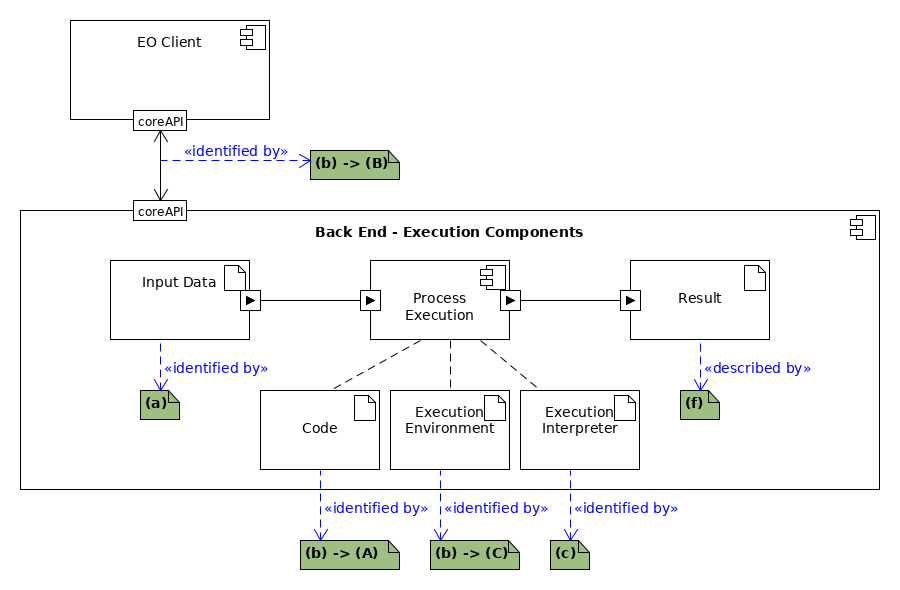
\includegraphics[width=\textwidth]{design_context_model}
	\caption{Overview of the backend execution components and the context model elements that identifies them.}
	\label{fig:design_contextmodel} 
\end{figure}

The backend provenance dataset contains job independent provenance and is identified by a backend version. Therefore, the necessary element of the backend provenance is the backend version that defines the state of the backend in a time period. The backend version must be resolvable by a code version present during a past execution. Besides, meta data about the backend can be added to the elements of the backend provenance. The elements ((A) - (D)) defined in Section \ref{Design:Backend provenance} are the suggestions of elements in the backend environment record. The following list recaps all of the backend environment elements: 

\begin{enumerate}[(A)]
	\item \textbf{Code identification} \\
	Enables the identification of the code of a backend version.
	\item \textbf{API version} \\
	Enables the identification of the API version of a backend version.
	\item \textbf{Backend version} \\ 
	Identifies the whole backend.
	\item \textbf{Publication timestamp} \\ 
	Enables the identification of a backend version at a specific time.
\end{enumerate}

The job execution context model, which includes all information related to a job execution, is stored in the context model. There are three necessary elements in the job context model. The input data identifier must be part of the context model, so that the input data of the job is identifiable. The backend version of the job execution must be included in the context model, to be able to re-execute it with the same backend state in the future. The job dependent context model must contain the output hash, so that differences in the job results are detectable. The following list recaps the elements of the job context model described in Section \ref{Design:Job dependent provenance}: 

\begin{enumerate}[(a)]
	\item \textbf{Input data persistent identifier} \\
	Identifies the input data of the job.
	\item \textbf{Backend provenance / code identifier} \\
	Identifies the backend version (C) during the execution of the job. Connects the job context model with the backend environment dataset.
	\item \textbf{Programming language} \\
	Identifies the programming language and version used by the job execution.
	\item \textbf{Dependencies of the programming language} \\
	Identifies the dependencies of the programming language used by the job execution.
	\item \textbf{Start and end time of process execution} \\
	Provides the start and end time of the job execution.
	\item \textbf{Result hash} \\
	Describes the results of the job execution.
\end{enumerate}

\section{User Services}\label{Design:User Interface}

This section describes the provided information for users and how users access it. The capturing described in the previous sections consist of information about the backends that backend provider do not want to pass entirely to users. For example, it can be risk to provide information on specific programming language packages if they have vulnerabilities. There is captured information that might not be necessarily useful for users. Therefore, there must be a filter on the shown information at the user services. The earth observation community has a diverse set of backends with unique company security guidelines.\\ 
Provenance information should be available to users to be useful. Therefore, we suggest additions to the backend API specification. It consists of additional endpoints for the users to get information about the backend and the client application. The following recommendations are for backend and client developer to make context model information accessible for users.

\begin{enumerate}[I.]
\item \textbf{Backend version} \\
	We suggest an endpoint to retrieve the backend specific information, especially the backend version. Additionally there need to be an endpoint to retrieve the backend version of a specific time. The aim of it is to present the users with information about the current state of the backend and to help users decide, which backend they want to use. 

\item \textbf{Detailed Job Information} \\
	We recommend an endpoint to retrieve detailed information about an already executed job. The endpoint includes the provenance of the job, therefore the resolvable persisted identifier of the input data, the backend version, and the result set hash. Additionally, the whole data of the context model can be made accessible, depending on the security decisions of the backend. \bgoesswein{We recommend to provide this information in PROV-O. In the current implementation the detailed job information can be accessed in PROV-JSON, PROV-XML or visualized exported as PNG (see Section \ref{Implementation:PROV-O}).}   
%\todo{I'd also add in the recommendation that this info should / could ideally be provided in PROV-O to ensure interoperability and standard compliance,butnot in this current imementation due to xxx (as discussed in Sec xxx) und}
\item \textbf{Comparing Two Jobs} \\
	We suggest an additional endpoint either on the backend or at the client application to compare two jobs. Every item of both of their context models is compared on equality. If they are not equal, the differences should be transparent to the user. The response of the comparison consists of the differences in the context model between two jobs. \bgoesswein{In this thesis this is the only comparison representation implemented. Future work will lead to a representation of the comparison according to PROV-O.}
%\todo{also.presented in PROV-O (?)}
\item \textbf{Data Identifier Landing Page} \\
	After the job is executed and the input data got an PID. The PID must be resolved by a \bgoesswein{machine-actionable} landing page. The landing page provides the user with information about the input dataset. We suggest an additional endpoint to re-execute the query showing the input data files if given sufficient permissions.
    
\item \textbf{Re-use of Input Data} \\
	We recommend to add the functionality to a backend to re-use input PIDs in a new job. The API allows to include the use of an input data PID in the process graph, so that users can include cited data directly in a newly created job description.   
\end{enumerate}

\section{User Defined Functions}\label{Design:User Defined Functions}
UDFs are customized code written by the user that gets executed in a virtualized environment at the backend provider. In theory, the user defines a docker base image and the code running in it. Therefore, it is a black box for the backend provider. They \bgoesswein{cannot} know how the code looks like in the docker container. Therefore, the capturing concept needs to be different than the typical way of executing jobs at the backend. The code and the docker base image has to be persisted by the backend provider. Additionally, the timestamp of the execution, to be able to identify the backend version at the execution. This is a rather new concept in earth observation science and not implemented on the EODC backend, hence the implementation of the capturing is not part of this thesis.

\section{Summary}
This chapter presented the design of the proposed solution. It shows how a backend can be extended to enable reproducible job executions. The data needed to be able to reproduce a job execution are presented and described. Data identification must be implemented according to the RDA recommendations. The elements of the backend environment are defined and are identifiable by the backend version. We defined the job dependent context by the job execution environment and the result hash. The data needed for a reproduction of a job execution is stored in the context model and it is the data needed to answer the research questions of Chapter \ref{Introduction}. In addition to the data description, recommendations on user services are listed. They provide the functionality for the users. The next chapter presents the implementation of the proposed design at the openEO compliant EODC backend.    

\chapter{Implementation}\label{Implementation}

In this chapter we present the \bgoesswein{implementation} of the thesis following the design described in Chapter \ref{Design}. It is implemented at the Python based EODC backend, a consortium member of the openEO project. The implementation consists of the suggested extensions to the backend and client application. It contains suggestions to the specification of openEO. Thus, we modify all three parts of the openEO project architecture in the presented solution. We modify the Python client\footnote{https://github.com/Open-EO/openeo-python-client} for the purpose of this thesis. \bgoessweindel{The motivation for choosing both of these options is that} Python is the most common programming language at the contributing backends of the openEO project. The implementation is open source and other backend providers with similar setup can use it.  

Similar to the design of this thesis, we structure the implementation in four parts presented in the first four sections. The first section describes the data identification implementation following the RDA recommendations at the backend. Section \ref{Implementation:Backend provenance} presents the implementation of the backend provenance capturing at the backend. Next, Section \ref{Implementation:Job dependent provenance} presents the implementation of the job dependent provenance at the backend. The last section describes the implementation of the proposed user services in the client application and the backend defined in Section \ref{Design:User Interface}.     
\newpage
\section{Data Identification}\label{Implementation:Data Identification}

In Section \ref{Design:Data Identification} we suggested that every backend provider has to implement data identification following the RDA recommendations. This section presents the data identification solution for the EODC backend. Other openEO backend providers can use the presented approach as well. This section focuses on the implementation of the core components on the backend. The mechanics of users getting and using the data identifier including the landing page is part of Section \ref{Implementation:User Interface}. \\

\subsection{Query Store}
The centerpiece of the RDA recommendations is the implementation of a Query Store. Queries in the Query Store must be comparable, identifiable, and persistent. The query data has to be stored at the backend infrastructure. The backend has a PostgreSQL database to store the executed jobs (see Figure \ref{fig:eodceer} in Section \ref{EODC Back End}). We realized the Query Store at the backend with two additional tables to this database. Figure \ref{fig:eer_rda} visualizes the proposed additional tables. The new \textit{Query} table consists of the query datarecord specified by the RDA recommendations. The \textit{QueryJob} table maps the relation between Job and Query. In the current version of the openEO core API, it is only possible to have one input data query used by a job. In the future, there may be the possibility to have more than one input data query related to one job execution. Hence we introduce the \textit{QueryJob} table. 

\begin{figure}[h]
	\centering
	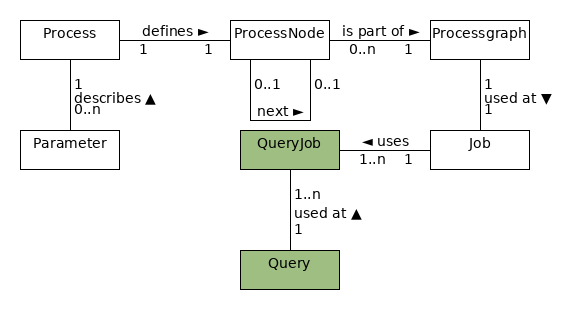
\includegraphics[width=\textwidth]{eodc_eer_rda}
	\caption{Overview of the database of the backend with the proposed additional tables (green).}
	\label{fig:eer_rda} % \label has to be placed AFTER \caption (or \subcaption) to produce correct cross-references.
\end{figure}

\subsection{Query Handler}
Figure \ref{fig:impldataid} shows an overview of the data identification solution at the backend. The green parts of the diagram represent proposed extensions. We implemented the \textit{Query Handler} component as an additional Python module in the backend called after the job execution. 

\begin{figure}[h]
	\centering
	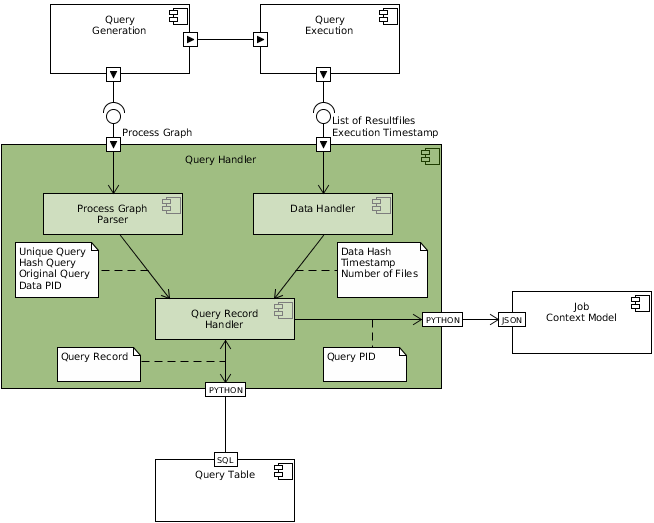
\includegraphics[width=\textwidth]{implementation_dataidentification}
	\caption{Overview of the proposed data identification component at the backend}
	\label{fig:impldataid} % \label has to be placed AFTER \caption (or \subcaption) to produce correct cross-references.
\end{figure}

The \textit{Query Generation} and \textit{Query Execution} components provide the input data of the \textit{Query Handler}. The process graph is the raw input process graph received by the backend driver from the client application. The list of result files is the result of the query execution and therefore, the input data of the job. The \textit{Query Execution} component provides the execution timestamp. The \textit{Query Handler} contains the following components:

 \begin{itemize}
	\item \textbf{Query Processor} \\
	The \textit{Query Processor} takes the executed query, parses and generates the necessary query data and forwards the information to the \textit{Query Record Handler}. This step is necessary, since the process graph at this point also includes the execution processes and not only the filter processes. The output is composed of the original query, the unique query, the hash of the unique query and the persistent data identifier (PID) of the query. This information is forwarded to the \textit{Query Record Handler}. The mentioned resulting items are described in more detail in the next section.   
	\item \textbf{Data Handler} \\ 
	The \textit{Data Handler} is responsible for creating the elements of a query record related to the query result. The output contains the hash over the file list, the execution timestamp and the number of resulting files. Since the backend uses the OGC standard CSW\footnote{http://cite.opengeospatial.org/pub/cite/files/edu/cat/text/main.html} to query the data, the sorting of the resulting files is predefined. The order of the files has no impact on the processing, and openEO users are not able to choose a sorting type. Therefore, the predefined CSW sorting is used for the hash production. The results of the \textit{Data Handler} component are forwarded to the \textit{Query Record Handler}.    
	\item \textbf{Query Record Handler} \\
	The \textit{Query Record Handler} communicates with the database of the backend to find existing identical query records. Figure \ref{fig:queryhandler_activity} gives an overview of the activities of the \textit{Query Record Handler}. If the query record already exists, the \textit{Query Record Handler} returns the existing PID, otherwise a new PID is created and the query is stored in a new query record. The combination of the result-file hash and the unique query hash must not have duplicates in the query table. On saving the query PID in the job context model, a queryjob record gets created. It sets the relation between the job execution and the input data query PID. 
\end{itemize}

\begin{figure}[h]
	\centering
	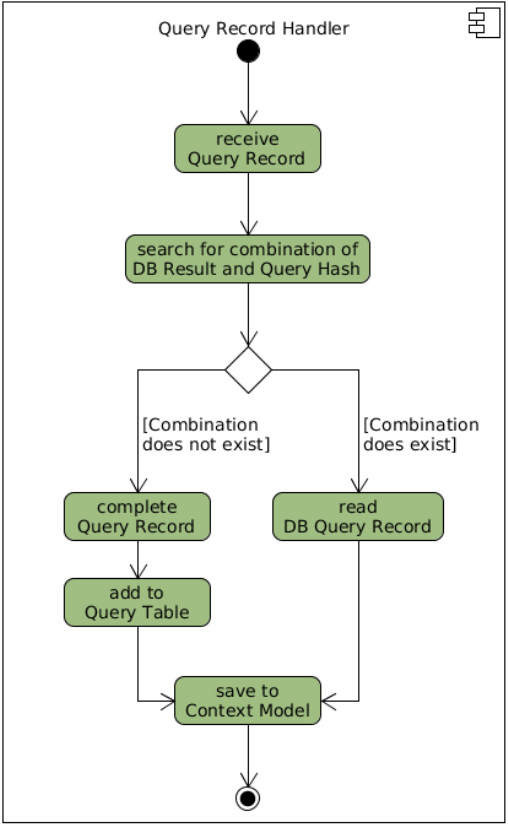
\includegraphics[scale=0.5]{queryhandler_activity}
	\caption{Activity diagram of the Query Record Handler component.}
	\label{fig:queryhandler_activity} % \label has to be placed AFTER \caption (or \subcaption) to produce correct cross-references.
\end{figure}

\subsection{Query Table Structure}

The query table stores the query data with additional result and data information. Table \ref{Tab:querytable} visualizes the structure of the query table. We added example values to explain how the parts of the query record are generated. Figure \ref{fig:processgraph_example} shows the example input process graph.   

\begin{figure}[h]
	\centering
	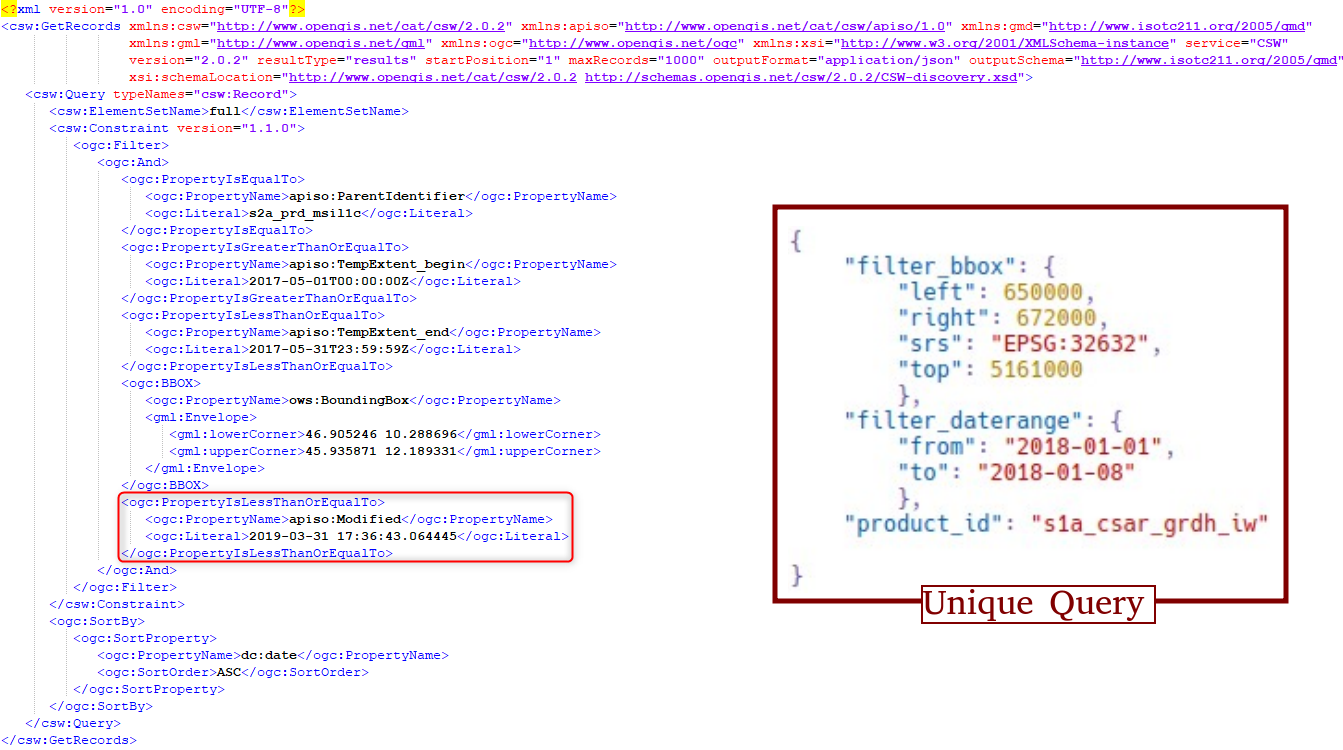
\includegraphics[width=\textwidth]{original_query}
	\caption{Example for the original query and the unique query of the example process graph.}
	\label{fig:processgraph_example} % \label has to be placed AFTER \caption (or \subcaption) to produce correct cross-references.
\end{figure} 

\begin{table}[]
	\caption{Structure of the Query Table in the PostGres database.}
	\begin{tabular}{|c|c|c|c|}%l|l|l|l|}
	\hline	\textbf{Query PID} & \textbf{Dataset PID} & \textbf{Original Query} & \textbf{Unique Query} \\ \textbf{} & \textbf{} & \textbf{} & \textbf{} \\ \hline VARCHAR(100) & VARCHAR(100) & TEXT & VARCHAR(300) \\ \hline \hline \textbf{Query Hash} & \textbf{Result Hash} & \textbf{Execution} & \textbf{Metadata}  \\ \textbf{} & \textbf{} & \textbf{Timestamp} & \textbf{}  \\ \hline
		 VARCHAR(65) & VARCHAR(65) & TIMESTAMP & TEXT \\ \hline
	\end{tabular}
	\label{Tab:querytable}
\end{table}

The following list describes how the elements of the query data set record are created in more detail:

\begin{enumerate}
	\item \textbf{Query PID} \\
	We generate the query PID with the Python library uuid\footnote{https://docs.python.org/3/library/uuid.html}. The library generates unique identifiers and the backend uses it for creating the job identifier. The identifier of the backend have codes related to the database table in the beginning (e.g. "jb-UUID" for job entities). That is why the id for the newly introduced query table is structured like "qu-UUID". \\
	\textit{Example: "qu-16fd2706-8baf-433b-82eb-8c7fada847da"}
	\item \textbf{Dataset PID} \\ 
	The dataset PID is the identifier of the satellite in the process graph (e.g. the identifier in the "load\_collection" process). \\
	\textit{Example: "s1a\_csar\_grdh\_iw"}	    	
	\item\textbf{Original Query} \\
	The initially executed CSW query of the query execution component.  \\ 
	\textit{Example: See the original query in Figure \ref{fig:processgraph_example}}	 
	\item \textbf{Unique Query} \\
	The unique query is the restructured query that is comparable to other unique queries. The order of the filters make no difference in the outcome of the query execution. Therefore, the filter arguments of the original query are alphabetically sorted by the JSON keys to generate the unique query. \\
	\textit{Example: See the unique query in Figure \ref{fig:processgraph_example}}	  	 	
	\item \textbf{Unique Query Hash} \\ 
	We remove newline and space characters from the unique query string. After that, we create the unique query hash by running the SHA-256 over the resulting unique query using the "hashlib" Python module.  \\
	\textit{Example: "AE7EF888CDEDF8A9A371\dots"} 
	\item \textbf{Result Hash} \\
	The result hash is the output of the SHA-256 hash function using the Python module "hashlib" over the result file list. \bgoesswein{The sorting of the files is fixed by the CSW query standard used by the backend.} We clean up the string of the file list by removing the newline and white space characters, before it is applied to the hash function. \\
	\textit{Example: "565D229FCE4772869343\dots"} 
	\item \textbf{Execution Timestamp} \\
	The execution timestamp is the input parameter of the \textit{Query Handler} transformed to the data type needed by the database. We take the timestamp from the \textit{Query Execution Handler} and is part of the result. \\
	\textit{Example: "2018-10-17 18:03:20,609"}  
	\item \textbf{Additional Data} \\
	The additional data column of the query table can be used by the backend to store additional information about the query execution. In the implementation of this thesis, we only store the number of output files. The column is defined as a JSON object and can be extended with additional data without changing the structure of the table. \\
	\textit{Example: "\{ "number\_of\_files": 10\}"}    	 
\end{enumerate}


\section{Backend Provenance}\label{Implementation:Backend provenance}

The backend provenance is idenfifyable by the backend version and contains the job independent provenance information. The following subsections explain how the (in Section \ref{Design:Backend provenance} defined) provenance data elements are implemented.  

\begin{enumerate}[(A)]
\item \textbf{GitHub Repository} \\
	The backend services deploy automatically from the GitHub repository. Therefore, we read the used GitHub repository information via the \gls{cli} of Git. We access the checked out commit and branch of the backend directly via the Git CLI, initiated with Python. Listing \ref{lst:impl_backendprov} shows the Git CLI calls used to retrieve the GitHub repository information needed by the backend provenance.      
\begin{code}
	\begin{minted}{bash}
	# Receiving the Git Repository URL
	git config --get remote.origin.url 
	# Receiving Branch
	git branch
	# Receiving the commit messages with the timestamps
	git log 
	\end{minted}
	\caption{Git CLI calls to get access the backend provenance.}
	\label{lst:impl_backendprov}
\end{code}

\item \textbf{Core API Version} \\
	The backend provider update the openEO core API version of the backend manually. The currently used API is in the GitHub repository of the backend. 

\item \textbf{Back End Version} \\
	The backend fetches the code for the services directly from GitHub and the Git commit identifies a certain state of the code. Therefore, we use the commit identifier as the version of the backend.

\item \textbf{Publication Timestamp} \\
	The publication timestamp of the version of the backend is defined by the timestamp when the Git commit happened. GitHub stores it and it can be retrieved via the Git CLI. 
\end{enumerate}

\section{Job Dependent Provenance}\label{Implementation:Job dependent provenance}
The backend transforms the process graph into separate docker containers. For every process in the process graph, there is a docker container running the Python implementation of the process. The input of the current process is the output of the previous process. The first process docker container has the input data defined in the process graph as input data, which is the result of the query execution. Every process saves the results in a temporary folder dedicated to the specific process execution. Every process has its temporary output directory until the whole process chain is finished. After that, the backend deletes the temporary folders, and it only keeps the result in the job directory.
The job must identify the input data, the output data and the execution environment to achieve the job environment data capturing described in Chapter \ref{Design:Job dependent provenance}. \\ 
The implementation adds the captured information to the logging of the job execution. After the job execution it reads the logging files to generate the context model. This solution extends the code of the backend with minor logging calls. Figure \ref{fig:impljobcapture} gives an overview of the implemented job capturing procedure. Section \ref{Implementation:Python Implementation} describes every part of the overview in more detail.

\subsection{Context Model Repository}\label{Implementation:Provenance Repository}
Each executed job generates a context model related to the job execution. If the job gets re-executed, the context model gets replaced by a new context model related to the later execution. The backend handles job re-executions as new jobs with the same process graph and assigns a new job identifier. Letting the same job be re-executed without creating a new job id is dropped from the agenda of the openEO project since version 0.3.1 (see the GitHub repository\footnote{https://open-eo.github.io/openeo-api/v/0.3.1/apireference/}).
The aim of this design decision is to turn the job id into an job execution identifier and the process graph to the identifier of a job. Therefore, different job ids with the same process graph represent different executions of the same job.
We store the context model formatted as a JSON object in the job execution database. After the job is carried out in the backend, the results are saved in a folder named after the job identifier and the meta data information is stored in the PostgreSQL database (see Section \ref{EODC Back End}). Jobs are stored in the \textit{Job} table of the database. We added an additional column to this table to store the context model in this solution. The creation of the context model is described with the implementation below. \\
Table \ref{Tab:contextmodel} provides the mapping between the context model elements from Section \ref{Design} and the keys of the JSON context model object of the prototype. The elements have a one to one mapping of the context model and the JSON key except for the timestamps of the execution. The execution timestamps are part of the \textit{Job} table in the EODC database. \\
Figure \ref{fig:job_context_model} shows an example context model. It consists of all elements described by the context model in the Design chapter. Information on the backend environment during the execution of the job is stored in the context model. We store the backend version and the execution timestamp in the context model to be able to identify backend provenance of the execution The code environment is a list of Python dependencies of the job execution with their versions. Besides, the Python interpreter version is added to the context model. How the data is captured in detail is described in the sections below.    
  
\begin{table}[]
	\caption{Relation of context model elements and the implementation JSON context model.}
	\begin{tabular}{l|l}
		\textbf{Context Model Definition} & \textbf{JSON Key} \\ \hline
		\textbf{(a): Input data persistent identifier} & input\_data \\ \hline
		\textbf{(b): Backend provenance / code identifier} & backend\_env \\ \hline
		\textbf{(c): Programming language} & interpreter \\ \hline
		\textbf{(d): Dependencies of the programming language} & code\_env \\ \hline
		\textbf{(e): Start and end time of the process execution} & start\_time, end\_time \\ \hline
		\textbf{(f): Result hash} & output\_data \\ %\hline
	%	\textbf{J7: Backend provenance} & backend\_env \\ 
	\end{tabular}
\label{Tab:contextmodel}
\end{table}

\begin{figure}[h]
	\centering
	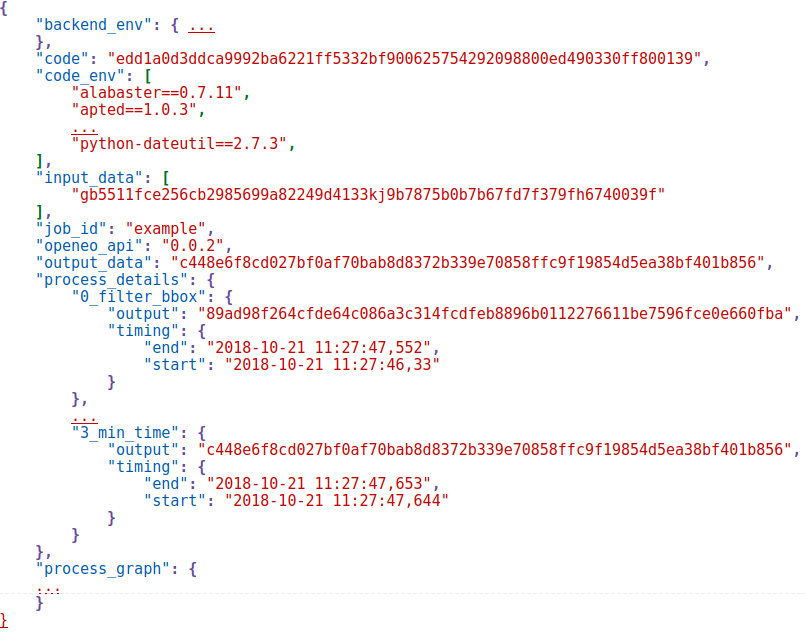
\includegraphics[width=\textwidth]{job_context_model}
	\caption{Example context model of a job execution at the backend implementation.}
	\label{fig:job_context_model} % \label has to be placed AFTER \caption (or \subcaption) to produce correct cross-references.
\end{figure}

\subsection{Python Implementation}\label{Implementation:Python Implementation}
The implementation of this thesis is an example for other backends with similar setups. Therefore, we implemented it in the Python version of the backend without any additional \bgoesswein{requironments on Python modules}. The Python solution uses logging messages to transfer the needed data from the process execution to the capturing modules. The cleanup service of the EODC backend driver triggers the modules of the solution. It is an additional Python module and parses the log files after the job is finished. This solution generates, except for the additional logging calls, little impact on the existing backend implementation. The EODC backend driver has already a logging system installed. Hence the modifications are added to the existing logging policy. \\
Figure \ref{fig:impljobcapture} visualizes the additional Python modules \textit{Job Capturing} and \textit{Result Handler} in the context of the backend environment. 

\begin{figure}[h]
	\centering
	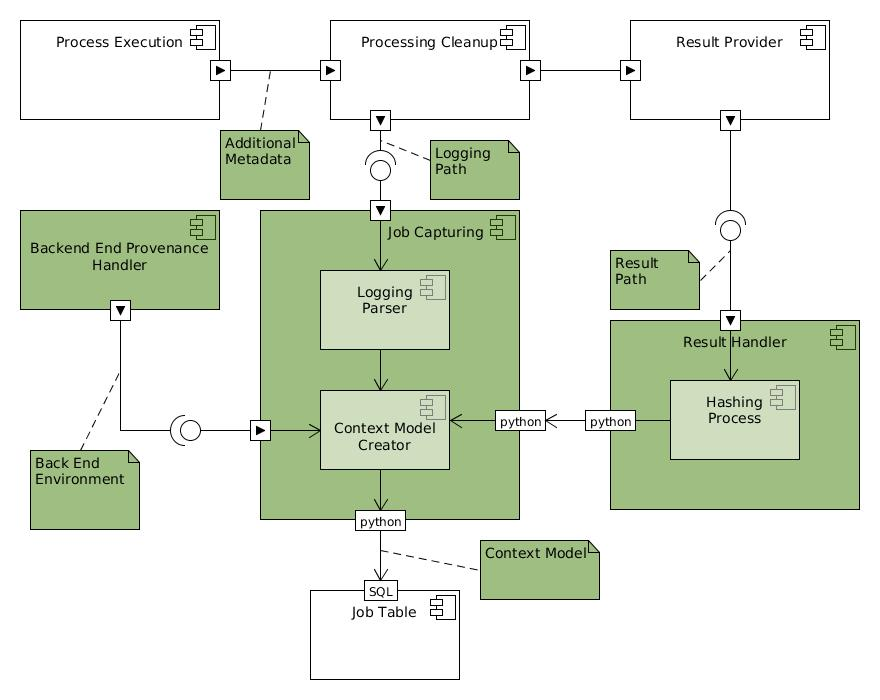
\includegraphics[width=\textwidth]{job_capturing_overview}
	\caption{Overview of the Job capturing architecture at the backend. Green blocks are additional modules}
	\label{fig:impljobcapture} % \label has to be placed AFTER \caption (or \subcaption) to produce correct cross-references.
\end{figure}

The following list describes the modules of the backend and the additional modules of the solution. The order of the list shows the order of the module execution. 

\begin{enumerate}
	\item \textbf{Process Execution} \\
	The \textit{Process Execution} module at the backend is responsible for the execution of the job. It creates the additional logging information (see (a), (c), (d) and (e) of the context model) and stores it in a logging file. 
	\item \textbf{Processing Cleanup} \\
	After finishing the job execution, the backend deletes all temporary folders from the file system and copies the results to the newly created job folder. Then the solution module \textit{Job Capturing} starts given the path of the logging file.  
	\item \textbf{Result Provider} \\
	The \textit{Result Provider} is responsible of making the result available for the user. It provides the user with information and feedback about the job execution. Additionally it invokes the \textit{Result Handler} module with the path of the resulting file.
	\item \textbf{Result Handler} \\
	The \textit{Result Handler} reads the result file and calculates an SHA-256 hash over it. After completion, it sends it to the \textit{Context Model Creator} module.  
	\item \textbf{Job Capturing} \\
	The \textit{Job Capturing} module parses the logging file to extract the information needed for the context model ((a), (c), (d) and (e)). It passes the rightful formatted information to the \textit{Context Model Creator}. The \textit{Context Model Creator} needs the \textit{Result Handler} (f) and \textit{Back End Provenance Handler} (b) for the remaining parts of the context model. After receiving all necessary information, the \textit{Context Model Creator} creates the JSON context model and saves it into the \textit{Job} table of the database.    
\end{enumerate}

The following sections describe the capturing of each data element of the job dependent context model in more detail.
\begin{enumerate}[(a)]
\item \textbf{Source Input Data Identifier} \\
	The source input data identifier is the PID of the input data provided by the query store described in Section \ref{Implementation:Data Identification}. It is forwarded to the \textit{Job Capturing} module by the \textit{Processing Cleanup} module. 

\item \textbf{Backend provenance / Code Identifier} \\
	The \textit{Job Capturing} module reads the backend provenance described in Section \ref{Implementation:Backend provenance}. The backend version active at the beginning of the execution is copied to the context model.

\item[(c)(d)] \textbf{Programming language and used libraries} \\
	The \textit{Process Execution} module uses the installed Python module \textit{pip} to list all installed packages with their versions. The module is at the moment used to manage the Python packages of the backend. The GitHub repository of the backend includes a Python environment file to install all needed dependencies of Python via \textit{pip} automatically. A feature of that tool is the \textit{pip freeze} call, which returns all installed Python packages with their versions. It is then transformed into a JSON object and saved to the context model. In addition to this the \textit{Process Execution} captures the Python version by using the \textit{sys.version} function of the \textit{sys} module. All of this executions are done in the \textit{Process Execution} module in the actual processing environment and stored in the output log file of the job execution.    

\item[(e)] \textbf{Start and end time of process execution} \\
	The start and end time of the process execution is already done by the backend in the  \textit{Process Execution} module. The resulting timestamps are persisted in the \textit{Job} table of the database. 

\item[(f)] \textbf{Result Identifier} \\
	The result identifier consists of the resulting data of the whole job execution. It is an SHA-256 hash (using the \textit{hashlib} Python library) of the resulting alphabetical sorted output files, which are placed in the resulting folder of the job execution directory. In the current version of the backend, there is only one result file created, due to the limitations of the available processes.   
\end{enumerate}

\section{User Services}\label{Implementation:User Interface}
The previous sections describe the technical insight of the backend. This section describes the implementation of the interfaces used by the users. Therefore, endpoints are added to the current existing openEO core API. Besides, the proposed endpoints are applied to the Python client and the backend. The implementation of the recommended additions of Section \ref{Design:User Interface} are described in the following:

\begin{enumerate}[I.]
\item \textbf{Backend version} \\
	We added a new endpoint for retrieving additional information about the backend. The new endpoint is a GET request with the path “/version” and no authentication is needed to access it. The response of the version endpoint is the job independent provenance information of the backend ((A)-(D), see Section \ref{Implementation:Backend provenance}). In a production version, the data may be filtered for information marked as a security risk. This endpoint is added to the backend to return the latest backend version. The endpoint takes a timestamp as parameter to get the backend version that was active at a specific time. We added a method to the Python client, so that the user can retrieve this information by calling “version()”. The result is a JSON object consisting of the backend provenance data. Listing \ref{lst:implementation_back_end_version} shows a result example.

\begin{listing}[ht]
	\begin{minted}{json}
{'branch': 'master',
'commit': '1a0cefd25c2a0fbb64a78cd9445c3c9314eaeb5b',
'url': 'https://github.com/bgoesswein/implementation_backend.git'}
	\end{minted}
	\caption{Backend version example.}
	\label{lst:implementation_back_end_version}
\end{listing}

\item \textbf{Detailed Job Information} \\
	In the openEO coreAPI, there is an endpoint for getting detailed information about a job execution. The endpoint path is “GET /jobs/<job\_id>” , which by the current release version (0.3.1) only contains the execution state of the job and the job id. In addition to this, we add the job dependent provenance to the endpoint (e.g. see Figure \ref{fig:job_context_model}). Since the Python client returns the resulting JSON response from the backend as a Python dictionary, there is no modification of the client needed. \bgoesswein{There is an option to retrieve the detailed job information in PROV-JSON format.}

\item \textbf{Comparing two Jobs} \\
	There does not exist any user interface to compare jobs in the coreAPI. The solution API defines a new endpoint in the manner of existing endpoint definitions. For this thesis, we introduce the endpoint  “POST /jobs/<job\_id>/diff”. In the URL of the request, the user defines the base job id, which context model is compared with other jobs. In the body of the request, the target job ids are defined in a JSON object. After getting the request from the user, the backend compares the context models of the base job with every target job occurring in the request body. The result from the backend consists of a term for every item in the base job context model. The term “EQUAL”, if the items are the same in both context models, the difference if the items are not the same in both context models, or \bgoesswein{“REMOVED”} if the item is in the base job context model, but missing in the target job context model, or \bgoesswein{"ADDED" if it is} the other way around. If an element is different, the elements that differ are visible. The latest mentioned outcome can occur if the context model definition is modified in future job executions and there are e.g. additional fields. The response contains the context model of all jobs with one of the previously described three states inside of the value of every item. In the Python client, this feature is added with an additional function of the Job class called "diff(target\_job)". Listing \ref{lst:job_comparison} provides an example of the dictionary output of this function.
%\todo{shouldn't these two cases be indicatex by different key terms? added/removed (in subsequent executions) rather than just stating missing, leaving it to the user to identify where it is missing?}
\begin{listing}[ht]
	\begin{minted}{json}
{
"process_graph":"EQUAL",
"input_data":"EQUAL",
"code_env":"EQUAL",
"output_data":"EQUAL",
"openeo_api":"EQUAL",
"back_end_timestamp": "REMOVED",
"end_time": "ADDED",
"different":{
   "interpreter": {"source": "Python 3.4", "target": "Python 3.5"},
   "job_id": {"source": "jb-47e062e4-d39c-4f7f-bc5e-aa877f039a84", 
              "target": "jb-b5e000f9-f586-40d1-b0b8-c813e5d93b4b"},
   "start_time": {"source": "2019-04-05 12:16:38.286217",
                  "target": "2019-04-05 13:14:22.369015"}}
}
	\end{minted}
	\caption{Example of a job comparison regarding the context model.}
	\label{lst:job_comparison}
\end{listing}	


\item \textbf{Data Identifier Landing Page} \\
	Depending on the backend, the input data may be restricted to the openEO interface. Therefore, the resolver of the input data PID is set within the coreAPI specification. There exists an endpoint to retrieve detailed information about a data set. We introduce the additional "GET /data/<data-pid>" endpoint. If the user calls the endpoint with a data PID, the result are the details of the underlying dataset and besides, the result of the query execution and the original query parameters \bgoesswein{in JSON format}. The landing page contains a link to another page with the file list after a query re-execution ("GET /data/<data-pid>/result" endpoint). If the result file list differs from the original execution, there is a list of the files that differ. Otherwise, it states that the file list is equal to the first execution. 

\item \textbf{Re-use of Input Data} \\
	To re-use the input data in different job execution, the client user can use the data PID in the process graph directly as source data, instead of just the unfiltered dataset identifier. If a process graph uses the input data PID, the backend automatically applies the queries in the way of the original execution. It is inserted in the process "get\_collection" as an additional filter argument named "data\_pid", to pass the data PID to the process graph. Section \ref{Implementation:Use Case1} provides an example of such a process graph. If the query result data changed from the original execution of the PID, the job shall be processed nonetheless, but a warning message appears to notify the user. \bgoesswein{The notification appears in the Python client, when the user fetches the result either automatically with synchronous jobs, or by a separate call in asynchronous jobs.}   
\end{enumerate}

\bgoesswein{
\subsection{PROV Modeling}\label{Implementation:PROV-O}

This section describes the mapping of the PROV elements with the provenance information of the job execution in the implementation. As mentioned in Section \ref{PROV} there are three core elements of the PROV-O annotation. The following enumeration shows how they are mapped with the job provenance information:

\begin{enumerate}
	\item \textbf{Entity element} \\
	We use entities to represent the data of the job execution. Therefore, we model the input data as well as the result data as entities. The PROV-DM definition specifies that an entity needs an identifier and can have additional attributes. We identify the input data with the query PID from the query store and set the entries of the query table as its attributes. The resulting entity is identified by the result hash and has no additional attributes. We set the type of both elements to "dataset".
	\item \textbf{Activity element} \\  
	An activity has an identifier, an optional start time, an optional end time and optional additional attributes. It takes entities and modifies them to generate new entities. We use the activity element to represent jobs. They are identified by the job id and have the additional information captured in the context model. The connection from the job to the entities is "used" for the input data and "wasGeneratedBy" for the result.
	\item \textbf{Agent element} \\
	Agents are capable of starting activities. In our solution we have two instances of agents. First, the user that starts the job execution. Second, the backend in which environment the job is executed. The user id identifies the user and the backend version identifies the backend. Since the backend does not start jobs on his own we add an "actedOnBehalfOf" relation between the backend and the user. We assign the type "Person" to the user and "SoftwareAgent" to the backend.    
\end{enumerate}

We implement the PROV-O representation with the "prov"\footnote{https://github.com/trungdong/prov} module for Python. It is capable of exporting the provenance in XML, JSON and RDF format. We also use the module to visualize the provenance. Figure \ref{fig:impl_provo} shows the PROV-O visualization of the example experiment. 
}
\begin{figure}[h]
	\centering
	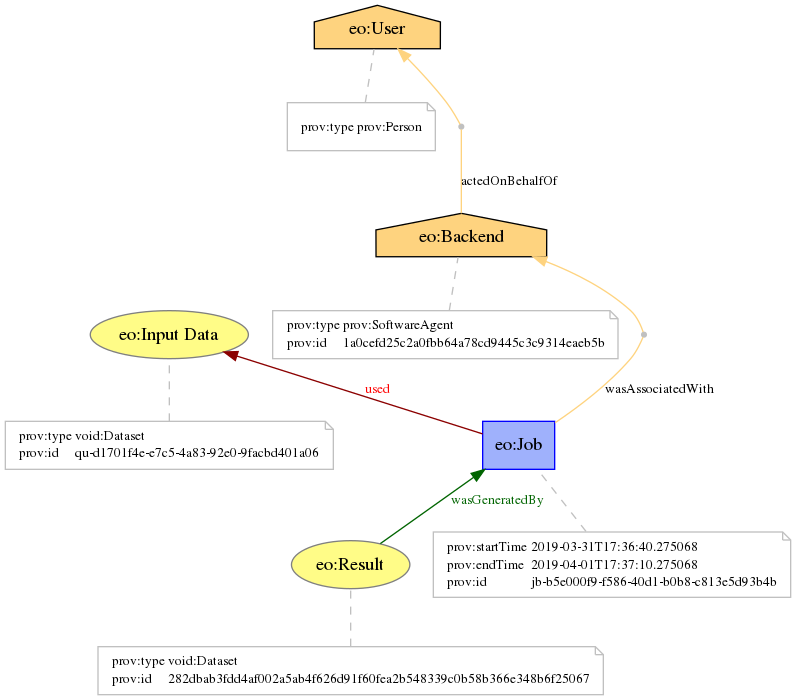
\includegraphics[scale=0.4]{provo}
	\caption{Example PROV-O representation of a job execution.}
	\label{fig:impl_provo} % \label has to be placed AFTER \caption (or \subcaption) to produce correct cross-references.
\end{figure}


\section{Use Cases}
This section shows how the use cases of Section \ref{Use Cases} are addressed using the implementation described in the sections before.

\subsection{Use Case 1 – Re-Use of Input Data}\label{Implementation:Use Case1}
The first use case describes how a researcher uses openEO as a processing environment. In this use case, the focus is on data identification and data citation. Researchers that use openEO may want to cite the data that is used in the applied job. Other scientists then want to use this data in their related research experiment. Section \ref{UseCase1} shows a step-by-step description of the use case. In this section, we execute the steps of the use case with the solution. The implementation of the use cases is available on GitHub\footnote{https://github.com/bgoesswein/dataid\_openeo/tree/master/openeo-python-client/examples}.

\begin{enumerate}
	\item \textbf{Researcher A runs an experiment (job A) at the EODC backend.} \\
	This step is basic openEO functionality and is not influenced by the solution from the user point of view. The researcher chooses Sentinel-2 data by loading the Sentinel-2 collection of the backend with the dataset identifier "s2a\_prd\_msil1c". In the next step, the researcher filters the collection data temporally (May of 2017) and spatially (bounding box of the South Tyrol area). In the next step the researcher applies the NDVI\footnote{https://earthobservatory.nasa.gov/features/MeasuringVegetation/measuring\_vegetation\_2.php} on the filtered data as well as the minimum value of each pixel during the time range with the "min\_time" process. The NDVI calculation needs the measurements of the satellite in near-infrared (parameter "nir") and the measurements of red light (parameter "red"). The backend represents the band identifiers of the two measurements by "B08" for near-infrared and "B04" for the visible red light. The last two lines create a job at the backend with the process graph and starts the execution of it at the backend.
	At the backend the \textit{Query Handler} generates a new data PID or returns an already existing one, if the same query was executed in the past. Listing \ref{lst:impl_usecase1_1} represents the experiment Python client code of Researcher A.
	
\begin{code}
	\begin{minted}{python}
import openeo
EODC_DRIVER_URL = "http://openeo.local.127.0.0.1.nip.io"

con = openeo.connect(EODC_DRIVER_URL)

# Choose dataset
processes = con.get_processes()
pgA = processes.get_collection(name="s2a_prd_msil1c")
pgA = processes.filter_daterange(pgA, extent=["2017-05-01", 
"2017-05-31"])
pgA = processes.filter_bbox(pgA, west=10.288696, 
south=45.935871, east=12.189331, 
north=46.905246, crs="EPSG:4326")

# Choose processes
pgA = processes.ndvi(pgA, nir="B08", red="B04")
pgA = processes.min_time(pgA)

# Create job A out of the process graph A (pgA)

jobA = con.create_job(pgA.graph)
jobA.start_job()
	\end{minted}
	\caption{Researcher A runs job A with the Python client.}
	\label{lst:impl_usecase1_1}
\end{code}	

\begin{figure}[h]
	\centering
	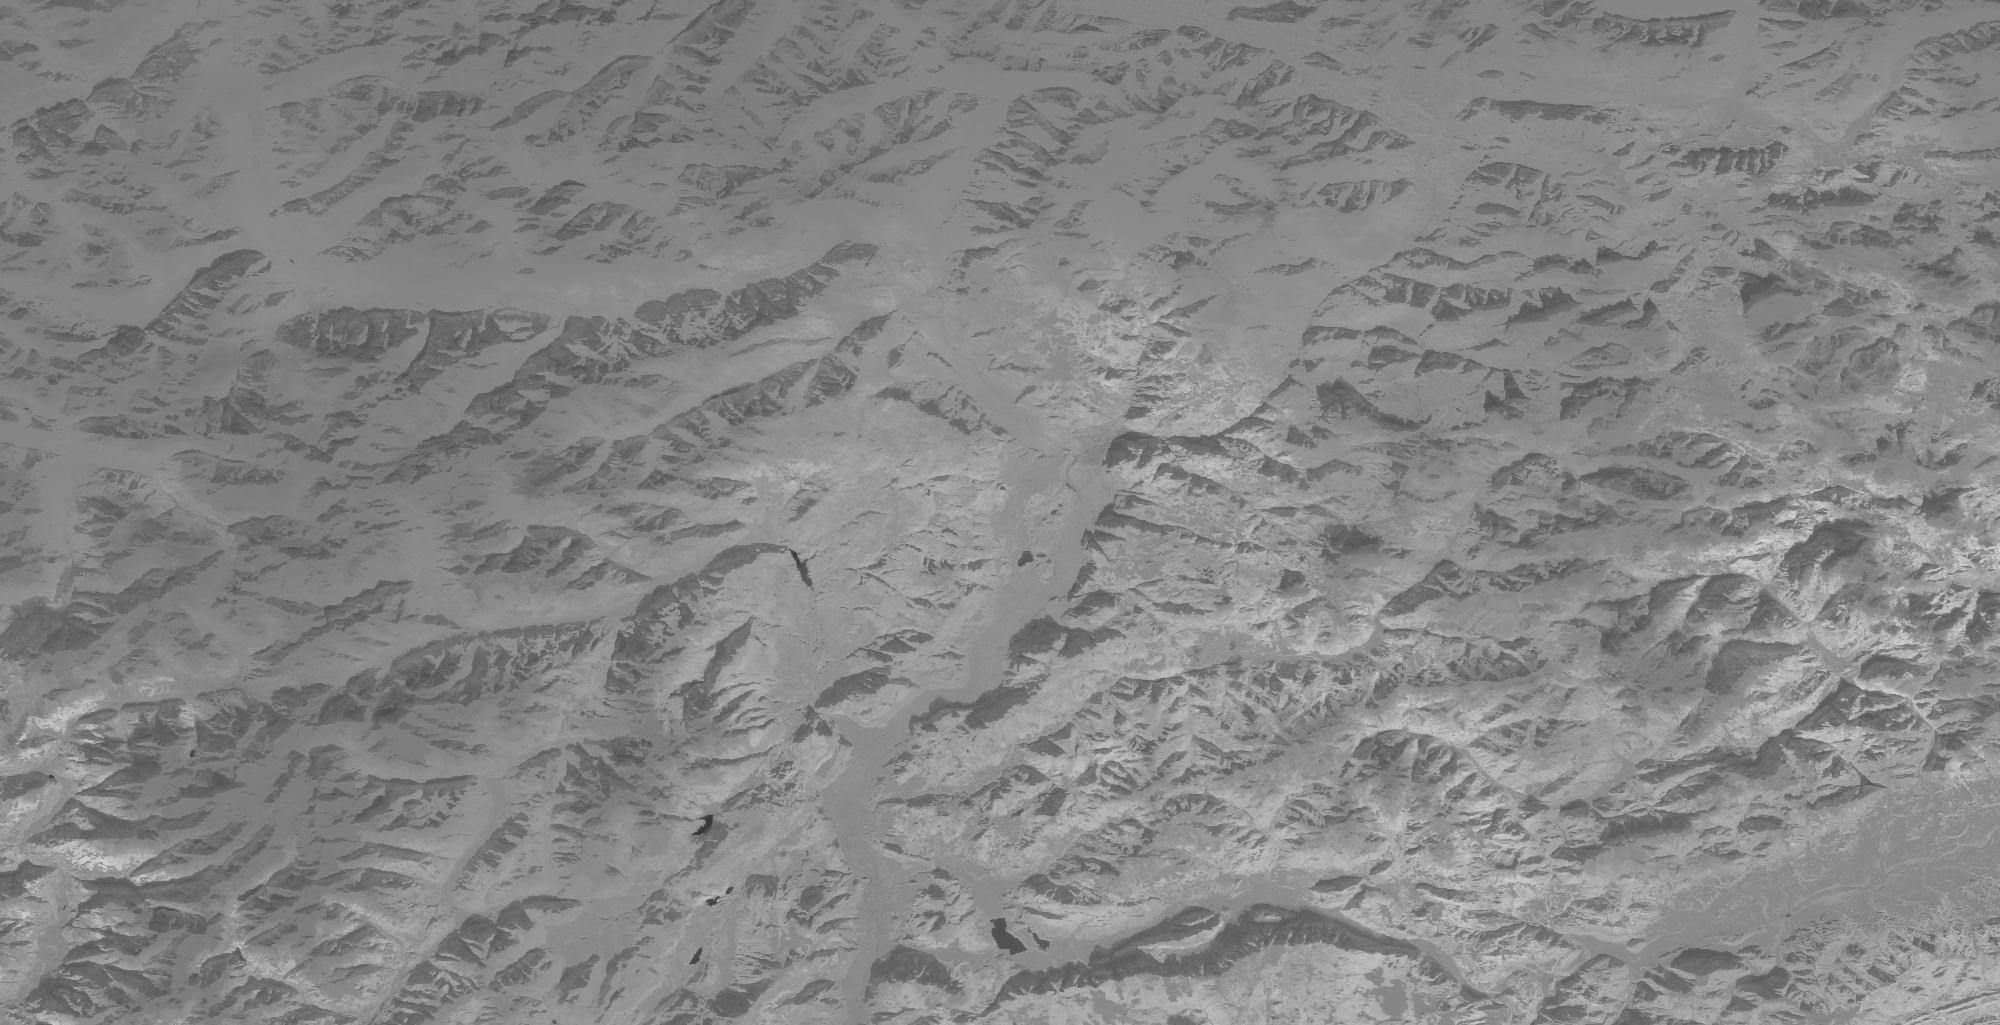
\includegraphics[width=\textwidth]{openeo_example_output}
	\caption{Resulting image of the first step of Use Case 1.}
	\label{fig:impl_usecase1_min} % \label has to be placed AFTER \caption (or \subcaption) to produce correct cross-references.
\end{figure}

	\item \textbf{Researcher A retrieves the used input data of job A.} \\
	Researcher A wants to receive the input data identifier by calling the job description endpoint. Listing \ref{lst:impl_usecase1_2} shows the calls used to do that with the Python client.

\begin{code}
	\begin{minted}{python}
pidA_url = jobA.get_data_pid_url()
print(pidA_url)
# Output: EODC_DRIVER_URL/data
#	/qu-d1701f4e-e7c5-4a83-92e0-9facbd401a06
pidA = jobA.get_data_pid()

# retrieve information about the pidA 
# e.g. executed query and description about the dataset.
desc = con.describe_collection(pidA)

query = desc["query"]
# re-execute query and get the resulting 
# file list from the backend
file_list = con.get_filelist(pidA)
	\end{minted}
	\caption{Researcher A retrieves the used input data PID.}
	\label{lst:impl_usecase1_2}
\end{code}
	
	\begin{figure}[h]
		\centering
		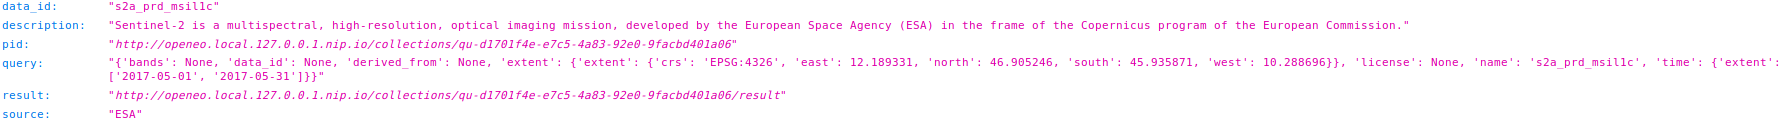
\includegraphics[width=\textwidth]{usecase1_2}
		\caption{Screenshot of the job A landing page.}
		\label{fig:usecase1-pid} % \label has to be placed AFTER \caption (or \subcaption) to produce correct cross-references.
	\end{figure}
	
	The job\_details variable is an JSON object that contains the response of the backend. It has a data element at the key of "input\_data" that contains the input data PID as a resolvable web address. Figure \ref{fig:usecase1-pid} shows the response data of the data PID information. After calling the page, the website provides the researcher with the executed filter parameter, the dataset identifier and a description of the dataset. Besides, the link to get the results of the query re-execution and the resolvable data PID are added to the page (see Figure \ref{fig:usecase1-pid}). \\
	The last three calls of the code block above are used to gather the information about the input data directly in the Python client code.  
	\todo{See Feedback --> Real Landing Page, with logo and so on...}
	\todo{result: what is this URL? Is it persisted? re-generted when entered into a browser? describe...}
	\todo{Relook the comments here}
	\item \textbf{Researcher A cites the input data in a publication.} \\
	This step is independent from the implementation and therefore not explained in detail. For the further steps it is assumed that Researcher A used the resolvable PID from step 2 (\textit{"BACKEND\_URL/data/qu-d1701f4e-e7c5-4a83-92e0-9facbd401a06"}) for the citation.   
	\todo{Make real citation, look at EODC /Copernicus how to do that}
	\todo{Feedback checked until here...}
	\item \textbf{Researcher B uses the same input data of job A for job B.} \\
	To use the same input data as Researcher A, Researcher B uses the data PID from the publication and puts it into the input data element of the process graph of job B. Listing \ref{lst:impl_usecase1_3} gives an example of the code needed to use the same input with a different process constellation (max\_time instead of min\_time process).  

\begin{code}
	\begin{minted}{python}
import openeo

# Take input data of job A by using the input data PID A
# pidA = qu-d1701f4e-e7c5-4a83-92e0-9facbd401a06
pgB = processes.get_data_by_pid(
data_pid="qu-d1701f4e-e7c5-4a83-92e0-9facbd401a06")
# Alternative: data_pid="EODC_DRIVER_URL/data/pidA" 

# Choose processes
pgB = processes.ndvi(pgB, nir="B08", red="B04")
pgB = processes.max_time(pgB)

# Create job B out of the process graph B (pgB)

jobB = con.create_job(pgB.graph)
jobB.start_job()
	\end{minted}
	\caption{Researcher B uses PID A for different job.}
	\label{lst:impl_usecase1_3}
\end{code}
	
\end{enumerate}

\begin{figure}[h]
	\centering
	
\includegraphics[width=\textwidth]{usecase1_max}
	\caption{Resulting image of the last step of Use Case 1.}
	\label{fig:impl_usecase1_max} % \label has to be placed AFTER \caption (or \subcaption) to produce correct cross-references.
\end{figure}
	
\subsection{Use Case 2 – Capturing job dependent environments}\label{Implementation:Use Case2}
This use case focuses on the execution environment. It handles the need of researchers to describe the execution environments of his experiments. Section \ref{UseCase2} describes the second use case in detail. The implementation at the backend gives the users the option to gain additional data about the execution. In the following, we show the implementation steps to realize the use case with our solution. 

\begin{enumerate}
	\item \textbf{Researcher runs an experiment (job A) at a backend.}\\
	The researcher A runs a job at the backend with the Python client code of Listing \ref{lst:impl_usecase2_1}.  It is the usual code of executing a job using the Python client. 

\begin{code}
	\begin{minted}{python}
import openeo
EODC_DRIVER_URL = "http://openeo.local.127.0.0.1.nip.io"

con = openeo.connect(EODC_DRIVER_URL)

# Choose dataset
processes = con.get_processes()
pgA = processes.get_collection(name="s2a_prd_msil1c")
pgA = processes.filter_daterange(pgA, extent=["2017-05-01", 
"2017-05-31"])
pgA = processes.filter_bbox(pgA, west=10.288696, 
south=45.935871, east=12.189331, 
north=46.905246, crs="EPSG:4326")

# Choose processes
pgA = processes.ndvi(pgA, nir="B08", red="B04")
pgA = processes.min_time(pgA)

# Create job A out of the process graph A (pgA)
jobA = con.create_job(pgA.graph)
jobA.start_job()
	\end{minted}
	\caption{Researcher A runs job A at the backend using the Python client.}
	\label{lst:impl_usecase2_1}
\end{code}

	\item \textbf{Researcher wants to describe the experiment environment.}\\
	The researcher wants to publish the result of the experiment and therefore, needs to describe the environment in detail. Listing \ref{lst:impl_usecase2_2} provides the code to give the user detailed information about the job A execution:

\begin{code}
	\begin{minted}{python}
# Get context model of job A
context_model = jobA.describe_job["context_model"]

# Retrieve the information that Researcher A needs.

interpreter = context_model["interpreter"]
code_env = context_model["code_env"]
input_data = jobA.get_data_pid_url()
backend_version = jobA.get_backend_version()
logging.info("Interpreter: {}".format(interpreter))
logging.info("Code Environment: {}".format(code_env))
logging.info("Input Data PID URL: {}".format(input_data))
logging.info("Back End Version (commit): {}"
             .format(backend_version["commit"]))
	\end{minted}
	\caption{Describe \textit{jobA} execution environment.}
	\label{lst:impl_usecase2_2}
\end{code}
\todo{remove logging Info lines and just output the whole thing...}
	After the execution of the lines above, the researcher can retrieve the used programming language and the installed packages with their versions. Besides, the backend version identifies the used code for the job execution. Listing \ref{lst:use_case2_logfile} shows the output of the logging calls.  
	
\end{enumerate}

\begin{code}
	\begin{minted}[fontsize=\footnotesize]{text}
INFO:root:Interpreter: Python 3.7.1
INFO:root:Code Environment: ['alembic==0.9.9', 'amqp==1.4.9',
         ..., 'GitPython==2.1.11', 'numpy==1.16.2', 'GDAL==2.4.0']
INFO:root:Input Data PID URL:
http://openeo.local.127.0.0.1.nip.io/collections
              /qu-8cdac780-7f47-4fac-9c4b-7a9ffff17d1d
INFO:root:Back End Version (commit): 
              16c3b32b5cb2d92d1c32d8c1f929065ee6bf2831
	\end{minted}
	\caption{Logging output of the second Use Case.}
	\label{lst:use_case2_logfile}
\end{code}
%\begin{figure}[h]
%	\centering
%	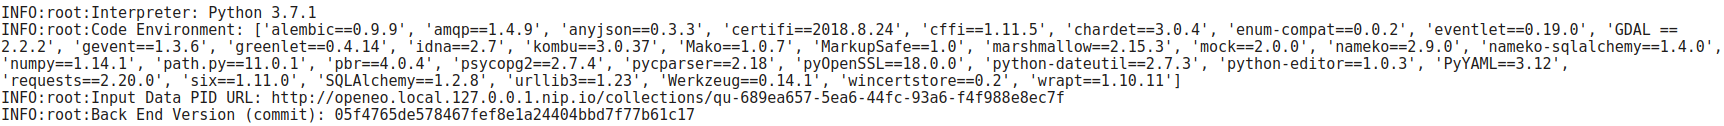
\includegraphics[width=\textwidth]{usecase2_2}
%	\caption{Screenshot of logging output of the second Use Case.}
%	\label{fig:usecase2_2} % \label has to be placed AFTER \caption (or \subcaption) to produce correct cross-references.
%\end{figure}

\subsection{Use Case 3 – Getting differences of job executions}\label{Implementation:Use Case3}
The last use case focuses on the users of openEO. It describes the need for transparency of job executions for the users. If results differ with the same job later in time, the user can access data to find reasons why it happened. Therefore, we use the new endpoint to compare job execution environments. Section \ref{UseCase3} describes the third use case in more detail.  
\begin{enumerate}
	\item \textbf{Researcher runs an experiment (job A) at a backend.}\\
	Listing \ref{lst:impl_usecase3_1} shows the Python code used by researcher A to run a new job at the backend. 

\begin{code}
	\begin{minted}{python}
import openeo
EODC_DRIVER_URL = "http://openeo.local.127.0.0.1.nip.io"

con = openeo.connect(EODC_DRIVER_URL)

# Choose dataset
processes = con.get_processes()
pgA = processes.get_collection(name="s2a_prd_msil1c")
pgA = processes.filter_daterange(pgA, extent=["2017-05-01", 
"2017-05-31"])
pgA = processes.filter_bbox(pgA, west=10.288696, 
south=45.935871, east=12.189331, 
north=46.905246, crs="EPSG:4326")

# Choose processes
pgA = processes.ndvi(pgA, nir="B08", red="B04")
pgA = processes.min_time(pgA)

# Create job A out of the process graph A (pgA)

jobA = con.create_job(pgA.graph)
jobA.start_job()
	\end{minted}
	\caption{Researcher A runs job A using the Python client.}
	\label{lst:impl_usecase3_1}
\end{code}

	\item \textbf{Researcher re-runs the same experiment (job B).}\\
	Listing \ref{lst:impl_usecase3_2} shows the re-execution of the same job e.g. by using the same process graph. The new execution gets a new job id and is called "job B" in the following.
\begin{code}
	\begin{minted}{python}
jobB = con.create_job(pgA.graph)
jobB.start_job()
	\end{minted}
	\caption{Researcher re-reruns job A resulting in job B.}
	\label{lst:impl_usecase3_2}
\end{code}
	\item \textbf{Researcher runs a different experiment (job C).}\\
	The researcher runs a third job (job C) with a different process graph and input data query. Listing \ref{lst:impl_usecase3_3} shows the code to create job C. 
\begin{code}
	%		\inputminted{octave}{BitXorMatrix.m}
	\begin{minted}{python}
# Choose dataset
processes = con.get_processes()
pgC = processes.get_collection(name="s2a_prd_msil1c")
pgC = processes.filter_daterange(pgC, extent=["2017-05-01", 
                                              "2017-05-31"])
pgC = processes.filter_bbox(pgC, west=10.288696, south=45.935871, 
                                 east=12.189331, north=46.905246, 
                                 crs="EPSG:4326")
	
# Choose processes
pgC = processes.ndvi(pgC, nir="B08", red="B04")
pgC = processes.max_time(pgC) # differs from job A
	
# Create job C out of the process graph C (pgC)
	
jobC = con.create_job(pgC.graph)
jobC.start_job()
	\end{minted}
	\caption{Researcher runs experiment different from job A.}
	\label{lst:impl_usecase3_3}
	
\end{code}

	\item \textbf{Researcher wants to compare the jobs by their environment and outcome.}\\
	Now the researcher wants to compare job B and job C with the original job A. Therefore he executes the code presented in Listing \ref{lst:impl_usecase3_4}.
	
	\begin{code}
%		\inputminted{octave}{BitXorMatrix.m}
		\begin{minted}{python}
diffAB = jobA.diff(jobB)
diffAC = jobA.diff(jobC)
logging.info("diffAB: \n {}".format(diffAB))
logging.info("diffAC: \n {}".format(diffAC))
		\end{minted}
		\caption{Researcher compares the different jobs.}
		\label{lst:impl_usecase3_4}
		
	\end{code}

	The researcher gets two dictionaries for the comparisons between job A with job B (diffAB) and job A with job C (diffAC). The content of the dictionary is a comparison of every key of the jobs context model. Listing \ref{lst:use_case3_logfile} shows the logging output of Listing \ref{lst:impl_usecase3_4} (using logging.info).
\end{enumerate}

%\begin{figure}[h]
%	\centering
%	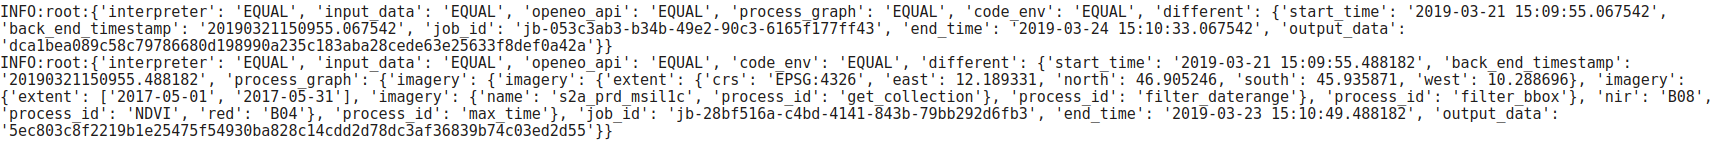
\includegraphics[width=\textwidth]{usecase3_4}
%	\caption{Logging output of the job comparisons diffAB and diffAC.}
%	\label{fig:eva_diff} % \label has to be placed AFTER \caption (or \subcaption) to produce correct cross-references.
%\end{figure}

\begin{code}
	\begin{minted}[fontsize=\footnotesize]{text}
INFO:root:diffAB:
 {'input_data': 'EQUAL', 'output_data': 'EQUAL', 
 'process_graph': 'EQUAL', 'openeo_api': 'EQUAL', 
 'interpreter': 'EQUAL', 'code_env': 'EQUAL',
 'different': 
 {'back_end_timestamp': {'target': '20190417194702.496810',
                         'source': '20190417154611.728540'}, 
 'job_id': {'target': 'jb-b92c688c-7fdc-4126-bcdf-85bc07030237',
            'source': 'jb-b5e000f9-f586-40d1-b0b8-c813e5d93b4b'}, 
 'start_time': {'target': '2019-04-17 19:47:02.496810',
                'source': '2019-04-17 15:46:11.728540'}, 
 'end_time': {'target': '2019-04-17 19:47:03.258261',
              'source': '2019-04-17 15:46:13.015937'}} 


INFO:root:diffAC:
 {'input_data': 'EQUAL', 'output_data': 'EQUAL', 
 'openeo_api': 'EQUAL', 'interpreter': 'EQUAL', 'code_env': 'EQUAL',
 'different': {'process_graph': { 'target': {'imagery': {'imagery': {'extent': 
 {'crs': 'EPSG:4326', 'east': 12.189331, 'north': 46.905246, 
 'south': 45.935871, 'west': 10.288696}, 'imagery': 
 {'extent': ['2017-05-01', '2017-05-31'], 
 'imagery': {'name': 's2a_prd_msil1c', 'process_id': 'get_collection'}, 
 'process_id': 'filter_daterange'}, 'process_id': 'filter_bbox'}, 
 'nir': 'B08', 'process_id': 'NDVI', 'red': 'B04'}, 'process_id':'max_time'}, 
 'source': {'imagery': {'imagery': {'extent': 
 {'crs': 'EPSG:4326', 'east': 12.189331, 'north': 46.905246, 
 'south': 45.935871, 'west': 10.288696}, 'imagery': 
 {'extent': ['2017-05-01', '2017-05-31'], 
 'imagery': {'name': 's2a_prd_msil1c', 'process_id': 'get_collection'}, 
 'process_id': 'filter_daterange'}, 'process_id': 'filter_bbox'}, 
 'nir': 'B08', 'process_id': 'NDVI', 'red': 'B04'}, 'process_id': 
 'min_time'}}, 
 'start_time': {'target': '2019-04-17 19:47:09.089075',
                'source': '2019-04-17 15:46:11.728540'}, 
 'end_time': {'target': '2019-04-17 19:47:11.786845',
              'source': '2019-04-17 15:46:13.015937'}, 
 'back_end_timestamp': {'target': '20190417194709.089075',
                        'source': '20190417154611.728540'}, 
 'job_id': {'target': 'jb-ecdd5768-3c22-4c73-85b8-ac6f4bdc138f',
            'source': 'jb-b5e000f9-f586-40d1-b0b8-c813e5d93b4b'}}
	\end{minted}
	\caption{Logging output of the job comparisons diffAB and diffAC.}
	\label{lst:use_case3_logfile}
\end{code}
%\todo{seperate logging info better, (maybe without Logging), show differences of both / use PROV O if possible. }
\section{Summary}
This chapter presented an implementation of the design of Chapter \ref{Design} at the EODC backend. It contains the implementation of the RDA recommendations. We implemented the query store with two additional tables at the database of the backend. We store the queries of the backend that follow the CSW\footnote{http://cite.opengeospatial.org/pub/cite/files/edu/cat/text/main.html} standard formatted in XML. The additional modules needed to achieve data identification are presented in Section \ref{Implementation:Data Identification}. Our implementation of the backend provenance uses GitHub as CVS to make the backend environment as well as the code for the job executions identifiable. We capture the job dependent environment by retrieving the Python environment using PIP. Our implementation uses the logging system of the backend to transfer the data to the additional modules. They create the context model by reading the logging files. The data of the query and the context model are stored in additions to the existing PostgreSQL database. Besides, the endpoints needed to access the provenance information lead to extensions of the openEO API. We implemented these extensions into the backend and the Python client. In the last section of the chapter, we present the code to run the use cases of Section \ref{Use Cases}. The following chapter evaluates the implementation by the impact on the EODC backend and by testing the implementation against exceptional cases.   

\chapter{Evaluation}\label{Evaluation}

This chapter evaluates the concept of the prototype implementation described in Chapter \ref{Implementation}. We evaluate the solution with test cases, which simulate updates on data as well as on the backend environment. After that, we evaluate the performance and storage impact of the implementation by applying 18 test cases derived from 9 publications that used EODC data in the past. The chapter is structured as follows: \\
First, we describe the setup of the evaluation environment in Section \ref{Evaluation:Setup}. Next, Section \ref{Evaluation:special_dataid} evaluates how the solution behaves on data updates at the backend. The following Section \ref{Evaluation:special_jobcap} evaluates the recreation of an older back end version using the solution. Section \ref{Evaluation:impact} provides measurements on the performance and storage impact of the prototype implementation. 

\section{Evaluation Setup}\label{Evaluation:Setup}

EODC uses an OpenShift\footnote{https://www.openshift.com/} service to manage the backends functionality. For this evaluation we installed OpenShift locally to run the backend with our extensions (furthermore called \textit{Solution Backend}). The data querying of EODC is publicly available and we use it in the evaluation. The \textit{Query Handler} component of the solution operates with the actual data of the backend provided for openEO users. \\
Figure \ref{fig:evaluation_setup} gives an overview of the evaluation setup. The job execution service of the backend cannot be executed locally, because data files are only inside the EODC infrastructure available. Therefore, the processing mechanism is mocked up by the \textit{Processing Mockup} component (see yellow box). It creates an array with mockup values in the size of the query results uses it for the process graph execution. The \textit{Solution Extensions} component (see green box) contains the backend extensions described in Chapter \ref{Implementation}. The \textit{Solution Python Client} is the openEO Python client with the extensions of Section \ref{Implementation:User Interface}, which give the user the possibility to operate with the proposed features via the Python client. The test cases are Python programs using the \textit{Solution Python Client} to create and execute jobs at the \textit{Solution Backend}.
We added a "reset" endpoint to the backend, to be able to run test cases independently. If called, it deletes all existing job and query records from the database. \\
Table \ref{Tab:eva_hardware} specifies the local machine used for the evaluation. To get a minimum performance bias, irrelevant background programs are disabled during the evaluation execution.\\  
The \textit{Solution Python Client}, the \textit{Solution Backend}, and the code for the evaluation is available and further described on GitHub\footnote{https://github.com/bgoesswein/dataid\_openeo}. 

\begin{figure}[h]
	\centering
	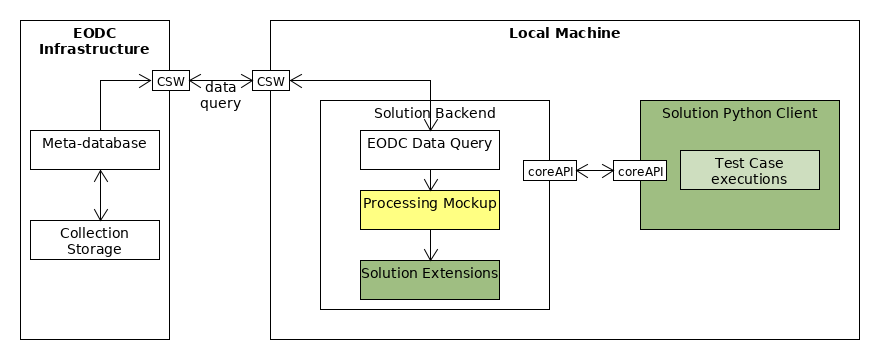
\includegraphics[scale=0.46]{evaluation_setup}
	\caption{Overview of the evaluation setup. Green boxes are components of the solution, white boxes are unmodified existing components and yellow boxes are components added only for the evaluation.}
	\label{fig:evaluation_setup} % \label has to be placed AFTER \caption (or \subcaption) to produce correct cross-references.
\end{figure}

\begin{table}[]
	\caption{Evaluation system specifications.}
	\centering
	\begin{tabular}{l|l}
		\multicolumn{2}{c}{\textbf{Hardware}} \\ \hline
		\textbf{\acrshort{cpu}} & Intel(R) Core(TM) i7-3770T CPU @ 2.50GHz \\ 
		\textbf{\acrshort{gpu}} & Radeon HD 7750/8740 / R7 250E  \\ 
		\textbf{\acrshort{ram}} & 16 GB  \\ 
		\multicolumn{2}{c}{\textbf{Software}} \\ \hline
		\textbf{\acrshort{os}} & Kubuntu 18.04.1 LTS \\ 
		\textbf{OpenShift} & 3.9.0  \\ 
		\textbf{Python} & 3.7.1  \\ 
	\end{tabular}
	\label{Tab:eva_hardware}
\end{table}
 
%\section{Special Test Cases}\label{Evaluation:special}
%This section evaluates special test cases to get an overview on how the solution behaves, if special circumstances on the backend occur. The GitHub repository of the solution has unit tests in the "test" folder of the python client testing the basic functionality. The test cases in this section are created to look into the error proneness of the solution. The code as well as the results of the evaluation in this section are available on GitHub\footnote{https://github.com/bgoesswein/dataid\_openeo/tree/master/openeo-python-client/examples/}.

\section{Data Identification}\label{Evaluation:special_dataid}
This section evaluates the data identification mechanism of the \textit{Solution Backend}. We first show how it fulfills the \acrshort{rda} recommendations. Next, we  show how the solution behaves if data updates or deletions occur at the backend.\\  
The policy of the EODC regarding updates on datasets is dependent on the type of data:

\begin{enumerate}
	\item \textbf{Sentinel Data} \\
	The Sentinel data, which is used by EODC for the openEO project, has never been updated before. The data comes directly from ESA, and updated datasets from ESA were not applied to the EODC data yet. However, the occurrence of updates is, in general, not impossible in future of the backend. If a dataset was updated, it would follow the updated policy of ESA, therefore having a new file name for the updated file. \bgoesswein{An update adds a new dataset record to the PostGIS database used for the data querying. It has the same attribute values as the original one, except for the new generated unique filename and the creation timestamp. In this solution we do not modify the PostGIS server of EODC. We simulate updates by modifying the query execution result.} Hence, we simulate updates on the data by renaming input files and their creation timestamp. Other than updating the existing datasets, there are regular updates on the extent of the Sentinel datasets.   
	\item \textbf{Processed Data} \\
	Data that is processed by partners of EODC is maintained and updated by the partners. EODC archives or deletes old versions depending on the decision of each partner. This type of data is not available using openEO, since it is the property of the partners and not EODC. Besides, to be able to use the same processes on different openEO backends, the data layer needs to be the same. Therefore, all openEO compliant backends provide unprocessed input data. Since the datasets are not available for openEO, the data identification of them is not in the scope of the thesis. By the time this thesis is written, EODC plans to use the openEO framework for their whole infrastructure, which brings the partners to use openEO for their processing. Therefore they can use the data identification implementation for their tasks.
\end{enumerate}

\subsection{RDA Recommendations}\label{Evaluation:dataidentification}
The Design (see Section \ref{Design:Data Identification}) proposes the implementation of the \acrshort{rda} data identification recommendations at the backend. Therefore, the following enumeration shows how we tackle the recommendations. 

\begin{itemize}
	\item \textbf{R1: Data Versioning} \\
	The backend does versioning of data already, by following the versioning policies of ESA. The path to a file represents the version identifier. Modified files must have a different file path.\bgoesswein{Every file has a data record in the PostGIS database, which stores the metadata e.g. timestamp of capturing and geographical extent. Every data record has an creation timestamp. It represents the time since the data record version is available at the backend. If a file is updated, the filename has to change as well as the creation timestamp. A query execution without filtering by the creation timestamp results in the file with the most recent creation timestamp. We filter by the creation timestamp to get the most recent file version of a specific time.}
	\item \textbf{R2: Timestamping} \\
	The creation timestamp of the files are stored by the file system of the backend and the PostGIS database. Since the files have to change the path after an update, the creation timestamp of the updated file is the update timestamp of the original file. 
	\item \textbf{R3: Query Store Facilities} \\
	We introduce a new table in the database (PostGreSQL) of the backend for the query store. The query table stores the following data about each query:
	\begin{itemize}
		\item The original \acrshort{csw} query in XML format
		\item The unique query: The backend generates the unique query using the filter arguments of the original query. It is then stored as a alphabetically sorted JSON object. 
		\item The hash of the unique query after removing characters with no semantic meaning.
		\item The hash of the alphabetically sorted resulting file list, after removing characters with no semantic meaning. 
		\item The timestamp of the original query execution.
		\item The dataset identifier is set to the used collection identifier of the query.
		\item The persistent identifier of the query generated using the UUID\footnote{https://docs.python.org/3/library/uuid.html} library of Python.
		\item A JSON object with the number of result files.
	\end{itemize}
	\item \textbf{R4: Query Uniqueness} \\
	The alphabetically sorted \bgoesswein{filter criteria} generated by the backend (See Figure \ref{fig:processgraph_example}).
	\item \textbf{R5: Stable Sorting} \\
	The original \acrshort{csw} query assures stable sorting. It alphabetically sorts the resulting file list in ascending order.
	\item \textbf{R6: Result Set Verification} \\
	The resulting file list is alphabetically sorted in ascending order. It transfers to a string object that cleaned up by not relevant characters, which we hash by the SHA-256 hash function. 
	\item \textbf{R7: Query Timestamping} \\
	The implementation stores the timestamp of the original query execution. 
	\item \textbf{R8: Query PID}\\
	The query PID is created using the Python UUID library if the same unique query and resulting hash combination is not in the database yet.
	\item \textbf{R9: Store the Query} \\
	We implemented the query store as an additional table of an existent relational database of the backend (PostgreSQL). 
	\item \textbf{R10: Automated Citation Texts} \\
	The citation text for the dataset is already available at EODC. We added the generated data PID. \todo{Link to automated citation text}
	\item \textbf{R11 \& R12: Landing Page \& Machine Actionability} \\
	We define the landing page as an additional openEO endpoint. It is publicly accessible and in a JSON format, which makes it machine actionable. The landing page includes a link to re-execute the query and lists the result files. Since it is part of the openEO API, it can also be accessed from the openEO clients and be used in future jobs as input data.
	\todo{Make Landing Page... and Link to it here}
	\item \textbf{R13 \& R14: Technology Migration \& Migration Verification} \\
	These recommendations are not implemented in this thesis, since there are no EODC migrations planned. \bgoesswein{Nevertheless, we estimate potential risks of a migration process. Using the Git commit as identifier of code might cause issues, when migrating to a different VCS. If the repository just moves to a different Git server, the whole history, including commit identifiers, can be migrated. There might be issues with the result hash, if the backend decides to change the format of the file paths. The creation timestamps of the datasets have to be migrated properly, since they are an important element of this solution.}
\end{itemize}

The original data of EODC can't be changed for this evaluation since the evaluation backend is using the actual data source (https://csw.eodc.eu). To simulate changes on the data, we modify the query result received by the backend. Figure \ref{fig:eva_data_simulation} gives an overview of where the data update simulator is located in the data identification implementation overview of Figure \ref{fig:impldataid}. The test cases describe what data is modified. \\
The test cases of the following sections focus on the Sentinel Data of EODC, and how the solution behaves on data updates. We use the running job (referenced as \textit{jobA}) defined in Section \ref{example} for the test case execution. Every test case starts with one executed job at an empty database. It stores the first query table entry. The next section describes how we achieve the initial test case state.

\begin{figure}[h]
	\centering
	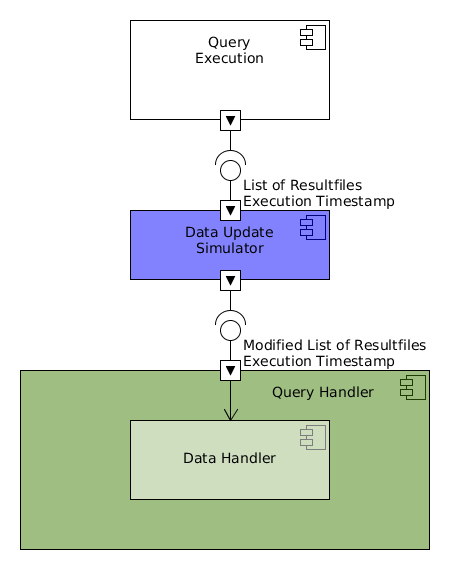
\includegraphics[scale=0.4]{evaluation_data_simulation}
	\caption{Overview of the data update simulation. It shows the extension on the data identification implementation of Figure \ref{fig:impldataid}.}
	\label{fig:eva_data_simulation} % \label has to be placed AFTER \caption (or \subcaption) to produce correct cross-references.
\end{figure}

\subsection{Test Case Preparation}
This section describes the test case preparation, so the step executed before every test case execution. It creates an initial job and input query entry, which is needed for the test cases. In the beginning the database is empty, we achieve this by calling the introduced reset endpoint. \\ 


\begin{enumerate}
	\item \textbf{Run \textit{jobA}, which creates query \textit{pidA}. Get result files of \textit{pidA}} \\
	Listing \ref{lst:eva_datachange_1} shows the code to run \textit{jobA} using the Python client. The researcher defines the spatial and temporal filter arguments and applies the NDVI and the "minimum time" process on it. This is the running example described in Section \ref{example}. The "con.create\_job()" call sends the process graph to the backend and retrieves a job object containing the newly generated job id. After executing \textit{jobA} (calling start\_job()), a job entity and a query entity are created and stored in the database. The query entity with a newly generated data PID is created by the \textit{Query Handler}. Table \ref{Tab:eva_datachanges1} shows the state of the query table after the execution of Listing \ref{lst:eva_datachange_1}.
	\begin{code}
		\begin{minted}[fontsize=\small]{python}
con = openeo.connect("http://openeo.local.127.0.0.1.nip.io")
# Choose dataset
processes = con.get_processes()
pgA = processes.get_collection(name="s2a_prd_msil1c")
pgA = processes.filter_daterange(pgA, extent=["2017-05-01", "2017-05-31"])
pgA = processes.filter_bbox(pgA, west=10.288696, south=45.935871, 
east=12.189331, north=46.905246, crs="EPSG:4326")
# Choose processes
pgA = processes.ndvi(pgA, nir="B08", red="B04")
pgA = processes.min_time(pgA)
# Create and start job A out of the process graph A (pgA)
jobA = con.create_job(pgA.graph)
jobA.start_job()
# Get data PID of jobA
pidA = jobA.get_data_pid()
# Re-execute the query to print the used files.
file_listA = con.get_filelist(pidA)
# Get state of the resultfiles, so if they changed since 
# the original execution 
file_listA["input_files"]["state"] # Returns "EQUAL"
		\end{minted}
		\caption{Researcher runs \textit{jobA} and retrieves the result files status.}
		\label{lst:eva_datachange_1}
	\end{code}

	Figure \ref{fig:eva_data_changes_1_query} shows the original query. It is has an XML format and contains the filter values defined in the process graph (pgA). Figure \ref{fig:eva_data_changes_1_query} highlights the timestamp of the first query execution. The content of the database tables as well as query re-execution results after each execution step are available in the result folder\footnote{https://github.com/bgoesswein/dataid\_openeo/tree/master/openeo-python-client/examples/results} of the GitHub repository. 
	
	\begin{figure}[h]
		\centering
		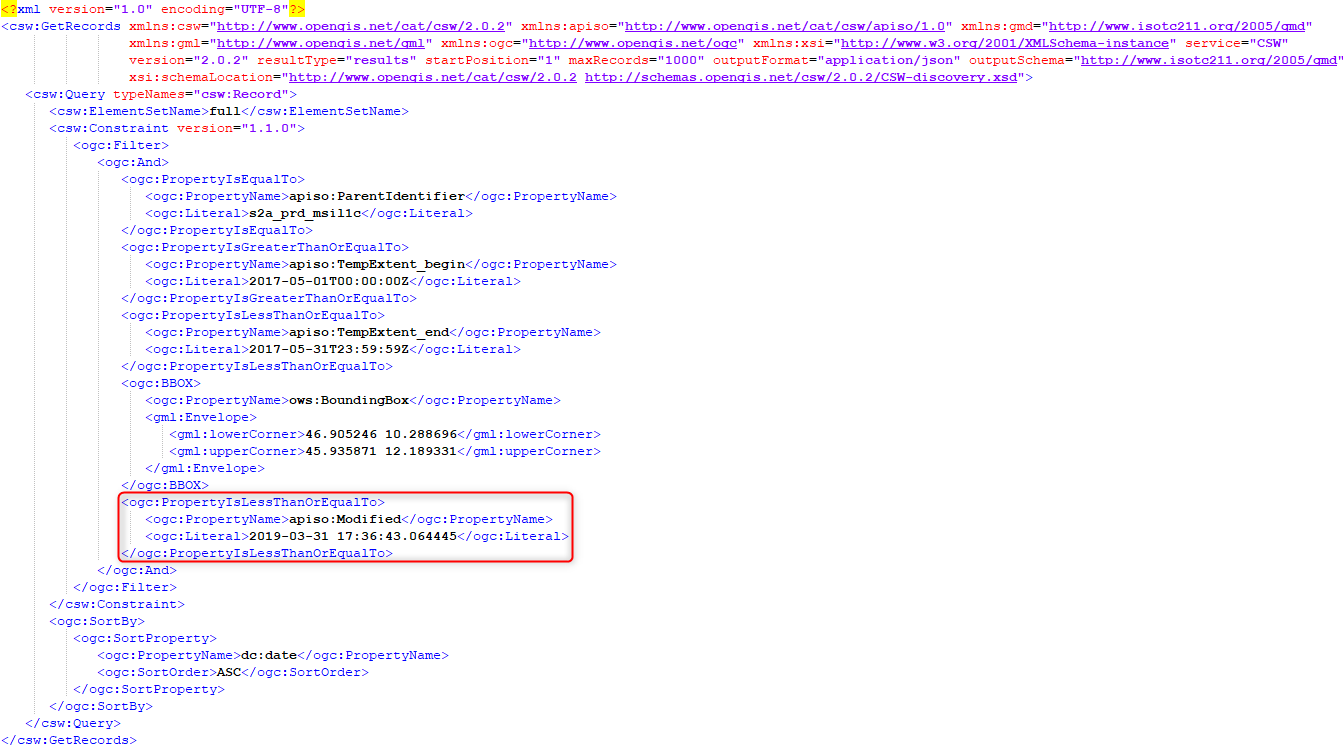
\includegraphics[width=\textwidth]{eva_data_changes_1_query}
		\caption{Original query of \textit{jobA} after the test case preparation step.}
		\label{fig:eva_data_changes_1_query} % \label has to be placed AFTER \caption (or \subcaption) to produce correct cross-references.
	\end{figure}
	
	Listing \ref{lst:eva_datachange_nq1} shows the normalized query created by the \textit{Query Handler}. It contains all filter arguments and their values in a JSON object alphabetically sorted. Note that filter options that the user does not use have a "None" value.
	
	\begin{code}
		\begin{minted}[fontsize=\footnotesize]{text}
{'bands': None, 
'data_id': None, 
'derived_from': None, 
'extent': {'extent': {'crs': 'EPSG:4326', 'east': 12.189331, 
'north': 46.905246, 'south': 45.935871, 'west': 10.288696}}, 
'license': None, 
'name': 's2a_prd_msil1c', 
'time': {'extent': ['2017-05-01', '2017-05-31']}}
		\end{minted}
		\caption{Normalized query of the initial query entry.}
		\label{lst:eva_datachange_nq1}
	\end{code}
	
	Listing \ref{lst:eva_datachange_rf1} shows the first four file paths and timestamps of the resulting file list, after executing the query of Figure \ref{fig:eva_data_changes_1_query}. \bgoesswein{The query in Figure \ref{fig:eva_data_changes_1_query} in XML format follows the CSW standard for EO web service catalogs. The backend sends it to the PostGIS server of EODC, which translates it to the SQL based internal query and executes it.} The resulting file list (file\_listA["input\_files"]) are 51 files and the re-execution of the query results in the same 51 files. The path of each file provides information about the data record. The term "s2a\_prd\_msil1c" defines the dataset identifier of Sentinel 2 at the backend. The following folders define the date of the data record. The filename follows the ESA naming convention\footnote{https://sentinel.esa.int/web/sentinel/user-guides/sentinel-2-msi/naming-convention}. The Nxxyy value defines the baseline number, Rxxx defines the orbit number of the satellite and Txxxxx defines the tile number. The first date is the sensing time and the second at the end of the file name is the product disclaimer, therefore distinguishes products that came from the data of the same sensing time. The timestamp shows when the data was first available at EODC.
	
	\begin{code}
		\begin{minted}[fontsize=\footnotesize]{text}
{'timestamp': '2017-05-08 00:00:00', 
'path': '/eodc/products/copernicus.eu/s2a_prd_msil1c/2017/05/04/
S2A_MSIL1C_20170504T101031_N0205_R022_T32TPR_20170504T101349.zip'}, 
{'timestamp': '2017-05-08 00:00:00',
'path':'/eodc/products/copernicus.eu/s2a_prd_msil1c/2017/05/04/
S2A_MSIL1C_20170504T101031_N0205_R022_T32TQS_20170504T101349.zip', 
{'timestamp': '2017-05-08 00:00:00', 
'path': '/eodc/products/copernicus.eu/s2a_prd_msil1c/2017/05/04/
S2A_MSIL1C_20170504T101031_N0205_R022_T32TQR_20170504T101349.zip'}, 
{'timestamp': '2017-05-08 00:00:00',
'path':'/eodc/products/copernicus.eu/s2a_prd_msil1c/2017/05/04/
S2A_MSIL1C_20170504T101031_N0205_R022_T32TPT_20170504T101349.zip'},
...
		\end{minted}
		\caption{First four resulting files with creation timestamp.}
		\label{lst:eva_datachange_rf1}
	\end{code}
	
	Table \ref{Tab:eva_datachanges1} shows the content of the query table after the execution of the test case preparation step. It has one entry with a new generated data PID, since there was no query entry before.
	
	%\begin{table}[]
	%	\caption{\textit{Query} table after the execution of Listing \ref{lst:eva_datachange_1}}
	%	\begin{tabular}{|l|l|l|l|l|l|l|l|l|}
	%		\hline	\textbf{query\_pid} & \textbf{dataset\_pid} & \textbf{original} & \textbf{normalized} & \textbf{norm\_hash} & \textbf{result\_hash} &
	%		\textbf{updated\_at} & \textbf{meta\_data} &   
	%		\textbf{created\_at} \\ \hline
	%		qu-a3bbe4a0-a875-4687-bb78-9457f33134a9 & s2a\_prd\_msil1c & see Figure \ref{fig:eva_data_changes_1_query} & see Listing \ref{lst:eva_datachange_nq1} & 0917c7a21cec960b8a6617b22ad26578c2c67f0b0501ba1a359b078c6c51d77d & abf43f519007050cbaeb59a067a2226d64b041c6d6ec323b2401109176e66455 & 2019-03-31 17:36:44.613893 & {'result\_files': 51} & 2019-03-31 17:36:43.064445 \\ \hline
	%	\end{tabular}
	%	\label{Tab:eva_datachanges1}
	%\end{table}
	
	\begin{table}[]
		\caption{Query table after the execution of Listing \ref{lst:eva_datachange_1}}
		\centering
		\begin{tabular}{|r|l|}
			\hline \multicolumn{2}{|c|}{\textbf{Query \textit{pidA}}} \\
			\hline \multicolumn{1}{|c|}{\textbf{Column}}  &  \multicolumn{1}{c|}{\textbf{Value}} \\ \hline
			Query PID & qu-a3bbe4a0-a875-4687-bb78-9457f33134a9  \\ 
			Dataset PID & s2a\_prd\_msil1c  \\ 
			Original Query & XML CSW query (see Figure \ref{fig:eva_data_changes_1_query})   \\
			Unique Query & Sorted filter criteria (see Listing \ref{lst:eva_datachange_nq1})  \\
			Query Hash & 0917c7a21cec960b8a6617b22ad26578c2c67f0b0501ba1a359b078c6c51d77d  \\
			Result Hash & abf43f519007050cbaeb59a067a2226d64b041c6d6ec323b2401109176e66455   \\
			Execution Timestamp & 2019-03-31 17:36:43.064445   \\ 
			Metadata & \{'result\_files': 51\}  \\ \hline
		\end{tabular}
		\label{Tab:eva_datachanges1}
	\end{table}
\end{enumerate}
\newpage
\subsection{Test Case 1: Is it possible to re-execute a query after a file is updated?}	\label{Tab:eva_datachanges_tc1}
%{ \large \textbf{} } \\

\begin{enumerate}
	\setcounter{enumi}{+1}
	\item \textbf{Update one of the resulting files of the \textit{pidA} query} \\
	We added the "update\_file()" method to the client and the backend to let the backend activate the \textit{Data Update Simulator} component shown in Figure \ref{fig:eva_data_simulation}. If it is activated, it simulates the update of the first file in the query result. It sets the creation timestamp of the file to the execution time of the "update\_file()" method and appends "\_new" to the file path. The update does not replace the old file but adds a new file to the result. Therefore, we simulate a new additional dataset record in the PostGIS database.
	\begin{code}
		\begin{minted}[fontsize=\small]{python}
# Update the first file of the pidA query resulting files.
con.update_file()
		\end{minted}
		\caption{Update one of the \textit{pidA} resulting files, but keep the original file.}
		\label{lst:eva_datachange_2}
	\end{code}
	
	Listing \ref{lst:eva_datachange_fl2} shows the result file list with the activated \textit{Data Update Simulator}. There is now an additional file with "\_new" at the end of the path, but with the same information in the file path and name as the first file. Besides, the creation timestamp is set to the time of the execution of Listing \ref{lst:eva_datachange_2}.	
	\begin{code}
		\begin{minted}[fontsize=\small]{text}
{'timestamp': '2017-05-08 00:00:00', 
'path': '/eodc/products/copernicus.eu/s2a_prd_msil1c/2017/05/04/
S2A_MSIL1C_20170504T101031_N0205_R022_T32TPR_20170504T101349.zip'}, 
{'timestamp': '2019-03-31 17:44:43', 
'path': '/eodc/products/copernicus.eu/s2a_prd_msil1c/2017/05/04/
S2A_MSIL1C_20170504T101031_N0205_R022_T32TPR_20170504T101349_new.zip'}
{'timestamp': '2017-05-08 00:00:00',
'path':'/eodc/products/copernicus.eu/s2a_prd_msil1c/2017/05/04/
S2A_MSIL1C_20170504T101031_N0205_R022_T32TQS_20170504T101349.zip', 
{'timestamp': '2017-05-08 00:00:00', 
'path': '/eodc/products/copernicus.eu/s2a_prd_msil1c/2017/05/04/
S2A_MSIL1C_20170504T101031_N0205_R022_T32TQR_20170504T101349.zip'}, 
{'timestamp': '2017-05-08 00:00:00',
'path':'/eodc/products/copernicus.eu/s2a_prd_msil1c/2017/05/04/
S2A_MSIL1C_20170504T101031_N0205_R022_T32TPT_20170504T101349.zip'},
...
		\end{minted}
		\caption{Modified file list output after the \textit{Data Update Simulator} component.}
		\label{lst:eva_datachange_fl2}
	\end{code}
	\item \textbf{Re-execution of \textit{pidA} query} \\
	Listing \ref{lst:eva_datachange_3} shows the re-execution of the query with the identifier \textit{pidA}, after the activation of the \textit{Data Update Simulator} component in the previous step. The second query re-execution results in the same file list as the first one (see Listing \ref{lst:eva_datachange_rf3}). The reason for this is that the old file is still available and the updated file is added after the execution timestamp of the original query execution (see timestamp element in the query in Figure \ref{fig:eva_data_changes_1_query}). The query from the query store contains the execution timestamp and keeps only the most recent file versions from that time. \todo{This does not seem to be correct. Please double-check and describe the implementation more precisely, showing details of the versioning and the actual query execution. If the above text were  correct (keeping all files with creation date before the execution date) you would run into problems ay soon as you have 2 updates on a file: this would potentially, return 2 old versions instead of the correct one  valid at the very moment of the original query execution. This is  CRITICAL! ease check and update.}
	\begin{code}
		\begin{minted}[fontsize=\small]{python}
# Get state of the resultfiles, so if they changed since 
# the original execution. 
file_listA = con.get_filelist(pidA)
file_listA["input_files"]["state"] # Returns "EQUAL"
		\end{minted}
		\caption{Re-execute \textit{pidA} query after one file got updated.}
		\label{lst:eva_datachange_3}
	\end{code}
	
	\begin{code}
		\begin{minted}[fontsize=\footnotesize]{text}
{'timestamp': '2017-05-08 00:00:00', 
'path': '/eodc/products/copernicus.eu/s2a_prd_msil1c/2017/05/04/
S2A_MSIL1C_20170504T101031_N0205_R022_T32TPR_20170504T101349.zip'}, 
{'timestamp': '2017-05-08 00:00:00',
'path':'/eodc/products/copernicus.eu/s2a_prd_msil1c/2017/05/04/
S2A_MSIL1C_20170504T101031_N0205_R022_T32TQS_20170504T101349.zip', 
{'timestamp': '2017-05-08 00:00:00', 
'path': '/eodc/products/copernicus.eu/s2a_prd_msil1c/2017/05/04/
S2A_MSIL1C_20170504T101031_N0205_R022_T32TQR_20170504T101349.zip'}, 
{'timestamp': '2017-05-08 00:00:00',
'path':'/eodc/products/copernicus.eu/s2a_prd_msil1c/2017/05/04/
S2A_MSIL1C_20170504T101031_N0205_R022_T32TPT_20170504T101349.zip'},
...
		\end{minted}
		\caption{First four resulting files of the file list.}
		\label{lst:eva_datachange_rf3}
	\end{code}

	\item \textbf{Run duplicate of \textit{jobA} named \textit{jobB}} \\
	Listing \ref{lst:eva_datachange_4} shows the execution of a second job using the same process graph as \textit{jobA}. In the first line of Listing \ref{lst:eva_datachange_4} the process graph of \textit{jobA} (defined in Listing \ref{lst:eva_datachange_1}) is used to create a new job instance named \textit{jobB}. Therefore, \textit{jobB} uses the same process graph as \textit{jobA} but gets executed after the update of the file in Listing \ref{lst:eva_datachange_2}. This is the common way of re-executing a job in openEO. This results in a different file list, where the original and the new file is in the query result file list (see Listing \ref{lst:eva_datachange_fl3}).
	\begin{code}
		\begin{minted}[fontsize=\small]{python}
# Reuse the defined process Graph (pgA) from jobA at Step 1 to create jobB
jobB = con.create_job(pgA.graph)
jobB.start_job()
# re-execute query and get the resulting file list from the backend
pidB = jobB.get_data_pid()
file_listB = con.get_filelist(pidB)
# comparing the resultfiles of jobA with the resultfiles of jobB
(file_listA == file_listB) # Returns False
		\end{minted}
		\caption{Step 4: Create \textit{jobB}, which uses the same process graph as \textit{jobA}.}
		\label{lst:eva_datachange_4}
	\end{code}
	
	\begin{code}
		\begin{minted}[fontsize=\small]{text}
{'timestamp': '2019-03-31 17:44:43', 
'path': '/eodc/products/copernicus.eu/s2a_prd_msil1c/2017/05/04/
S2A_MSIL1C_20170504T101031_N0205_R022_T32TPR_20170504T101349_new.zip'},
{'timestamp': '2017-05-08 00:00:00', 
'path': '/eodc/products/copernicus.eu/s2a_prd_msil1c/2017/05/04/
S2A_MSIL1C_20170504T101031_N0205_R022_T32TPR_20170504T101349.zip'}, 
{'timestamp': '2017-05-08 00:00:00',
'path':'/eodc/products/copernicus.eu/s2a_prd_msil1c/2017/05/04/
S2A_MSIL1C_20170504T101031_N0205_R022_T32TQS_20170504T101349.zip', 
{'timestamp': '2017-05-08 00:00:00', 
'path': '/eodc/products/copernicus.eu/s2a_prd_msil1c/2017/05/04/
S2A_MSIL1C_20170504T101031_N0205_R022_T32TQR_20170504T101349.zip'}, 
{'timestamp': '2017-05-08 00:00:00',
'path':'/eodc/products/copernicus.eu/s2a_prd_msil1c/2017/05/04/
S2A_MSIL1C_20170504T101031_N0205_R022_T32TPT_20170504T101349.zip'},
...
		\end{minted}
		\caption{Resulting file list of \textit{jobB}.}
		\label{lst:eva_datachange_fl3}
	\end{code}
	
	Table \ref{Tab:eva_datachanges3} shows the query table after the execution of Listing \ref{lst:eva_datachange_4}. Now there is an additional query entry. Table \ref{Tab:eva_datachanges3} marks the important differences red. There is a different result hash, because the \bgoesswein{resulted file name of the updated file is set to the most recent one}. The normalized query is still the same, but the result of the query changed therefore, a new data PID is generated. 
	\begin{table}[]
		\caption{Query table after the execution of Listing \ref{lst:eva_datachange_4}. Important elements are highlighted blue if they are the same and red if they are different.}
		\centering
		\begin{tabular}{|r|l|}
			\hline \multicolumn{2}{|c|}{\textbf{Query \textit{pidA} (full entry in Table \ref{Tab:eva_datachanges1})}} \\
			\hline \multicolumn{1}{|c|}{\textbf{Column}}  &  \multicolumn{1}{c|}{\textbf{Value}} \\ \hline
			Query PID & {\color{red}qu-a3bbe4a0-a875-4687-bb78-9457f33134a9}  \\ 
			Query Hash & {\color{blue}0917c7a21cec960b8a6617...}  \\
			Result Hash & {\color{red}abf43f519007050cbaeb59...}   \\
			Metadata & \{'result\_files': 51\}  \\
			\hline \multicolumn{2}{|c|}{\textbf{Query \textit{pidB}}} \\
			\hline \multicolumn{1}{|c|}{\textbf{Column}}  &  \multicolumn{1}{c|}{\textbf{Value}} \\ \hline
			Query PID & { \color{red} qu-23f5a313-e804-4faa-aa33-60ed1ac69e2d}  \\ 
			Dataset PID & s2a\_prd\_msil1c  \\ 
			Original Query & \textit{see Figure \ref{fig:appendix_pidB} in the appendix} \\
			Unique Query & \textit{see Listing \ref{lst:eva_datachange_nq1}}  \\
			Query Hash & {\color{blue}0917c7a21cec960b8a6617...}  \\
			Result Hash & {\color{red}28088d113de19ce037e965...}  \\
			Metadata & \{'result\_files': 51\}  \\
			Execution Timestamp & 2019-03-31 18:01:47.695042   \\ \hline
		\end{tabular}
		\label{Tab:eva_datachanges3}
	\end{table}
	
	\item \textbf{Run duplicate of \textit{jobA} named \textit{jobC}, by using the data PID of \textit{jobA} }\\
	The persistent input data identifier of job A (\textit{pidA}) is used as the input data for \textit{jobC}. The execution timestamp is part of the query entry behind \textit{pidA}, and the backend executes the original query for \textit{jobC}. \textit{jobC} uses the same data PID as \textit{jobA} therefore, the updated file is not in the result file list and there is no new data PID generated. The query table is still in the state of Table \ref{Tab:eva_datachanges3}. 
	\begin{code}
		\begin{minted}[fontsize=\small]{python}
# Take input data of job A by using the input data PID A of job A
pgC = processes.get_data_by_pid(data_pid=pidA)
# Choose processes
pgC = processes.ndvi(pgC, nir="B08", red="B04")
pgC = processes.min_time(pgC)
# Create and start Job C
jobC = con.create_job(pgC.graph)
jobC.start_job()
# re-execute query and get the resulting file list from the backend
pidC = jobC.get_data_pid()
file_listC = con.get_filelist(pidC)
# Compare resulting files with the original execution of jobA
(file_listA == file_listC) # Returns True
		\end{minted}
		\caption{Create \textit{jobC}, which uses the input data identified by \textit{pidA}.}
		\label{lst:eva_datachange_5}
	\end{code}
\end{enumerate}

Table \ref{Tab:eva_datachanges4} presents the mapping between the executed jobs and the input data PIDs of the first test case. The results are consistent if files are updated at the backend. Jobs using the original data PID (\textit{jobC}), also use the data defined by the PID, even after the update. The reason for this is the original file was still available. The current way of reproducing a job in openEO, by applying the same process graph (\textit{jobB}), fails since the resulting files differ from the first execution (\textit{jobA}). The query execution timestamp information is missing. Hence, the input data of \textit{jobB} result in a different data PID.       

\begin{table}[]
	\caption{Resulting mapping of the jobs and the used data PID of the first test case.}
	\centering
	\begin{tabular}{|r|l|}
		\hline \multicolumn{1}{|c|}{\textbf{Job}}  &  \multicolumn{1}{c|}{\textbf{Query PID}} \\ \hline
		\textit{jobA} & qu-a3bbe4a0-a875-4687-bb78-9457f33134a9  \\ 
		\textit{jobB} & qu-23f5a313-e804-4faa-aa33-60ed1ac69e2d \\
		\textit{jobC} & qu-a3bbe4a0-a875-4687-bb78-9457f33134a9  \\ \hline
	\end{tabular}
	\label{Tab:eva_datachanges4}
\end{table}
\newpage
\subsection{Test Case 2: Is it possible to re-execute a query after a file is updated with the original one deleted?}

\begin{enumerate}
	\setcounter{enumi}{+1}
	\item \textbf{Update one of the resulting files of the \textit{pidA} query and remove the original one.}\\ 
	The method in Listing \ref{lst:eva_datachange_6} updates the first file of the query result as described in Section \ref{Tab:eva_datachanges_tc1} and removes the original file. Listing \ref{lst:eva_datachange_fl4} shows the updated file list, where the first entry replaced the original first file (see Listing \ref{lst:eva_datachange_fl2}).
	\begin{code}
		\begin{minted}{python}
		con.update_file(deleted=True)
		\end{minted}
		\caption{Update one of the \textit{pidA} resulting files and delete the original file.}
		\label{lst:eva_datachange_6}
	\end{code}
	
	\begin{code}
		\begin{minted}[fontsize=\small]{text} 
{'timestamp': '2019-03-31 17:44:43', 
'path': '/eodc/products/copernicus.eu/s2a_prd_msil1c/2017/05/04/
S2A_MSIL1C_20170504T101031_N0205_R022_T32TPR_20170504T101349_new.zip'}
{'timestamp': '2017-05-08 00:00:00',
'path':'/eodc/products/copernicus.eu/s2a_prd_msil1c/2017/05/04/
S2A_MSIL1C_20170504T101031_N0205_R022_T32TQS_20170504T101349.zip', 
{'timestamp': '2017-05-08 00:00:00', 
'path': '/eodc/products/copernicus.eu/s2a_prd_msil1c/2017/05/04/
S2A_MSIL1C_20170504T101031_N0205_R022_T32TQR_20170504T101349.zip'}, 
{'timestamp': '2017-05-08 00:00:00',
'path':'/eodc/products/copernicus.eu/s2a_prd_msil1c/2017/05/04/
S2A_MSIL1C_20170504T101031_N0205_R022_T32TPT_20170504T101349.zip'},
...
		\end{minted}
		\caption{Modified file list output of the \textit{Data Update Simulator} component, by removing the original file from the list.}
		\label{lst:eva_datachange_fl4}
	\end{code}	

	\item \textbf{Get File-list of \textit{pidA}}\\ 
	The re-execution of the query \textit{pidA} results in a file list without the deleted file. Since files are filtered by the query execution timestamp. The new file does not appear in the result file list. \bgoesswein{If the re-execution results not in the same file list, the "state" attribute contains "Incomplete Result" and a list of files that replaced no longer available files are stored in the "diff" attribute.} Listing \ref{lst:eva_datachange_state} shows the content of the "diff" attribute of Listing \ref{lst:eva_datachange_7}. The backend returns the most recent file version, even if there are versions between the original and the most recent file available. In the result of Listing \ref{lst:eva_datachange_7} the "diff" contains only the one file that replaces the original file. Users can see the alternatives for the original file, but not the original file itself. This is because the full file list is not persisted in the query store, but the number of result files. The decision for not storing the complete file list was made by EODC. The reason is because of the additional needed storage size it would cause and the rare occasion of a data update. If the number of resulting files is different at a re-execution, we execute the query without the timestamp filter, and the result is compared to the re-execution with the original execution timestamp. All files that are missing in the original execution are added to the "diff" attribute. The researcher can use the file path to contact EODC or ESA to order older version.   
\todo{this feels plausible, but I am not sure whether I fully understand it.Query is executed with originL timestamps.As the number of resukt files differsandfhe hash key does not match, fhe user is informed that something went wrong --> how? is this the 'status" field (which, as the name indi ates, should report a status, not a file list!But then you also seem to be able to tell the user which file(s) are wdong, differsnt, missing - how do you do this??? Assumea scenario where in a result set of 10 files 5 files are changed, of which two have been deleted out of some reason - hoa do yoh identify which two files are different? Via the metadata database that still has the original filenames of the data repository? I seem to be missing something...}
	\begin{code}
		\begin{minted}[fontsize=\small]{python}
# re-execute query and get the resulting file list from the backend
file_listA = con.get_filelist(pidA)
# Stdout: Warning: The resulting file list changed from the original query
# execution! Look into the "diff" attribute to see the list of files that
# have changed. The original data might be still obtainable by the original data provider. Please contact the backend provider for further information.
file_listA["input_files"]["state"] # Returns "Incomplete Result"
file_listA["input_files"]["diff"] # Returns one file entry
		\end{minted}
		\caption{Re-execute \textit{pidA} query after one file is updated and the old version is erased.}
		\label{lst:eva_datachange_7}
	\end{code}	
	\todo{Feedback bis hierher berücksichtigt}
	%\begin{figure}[h]
	%	\centering
	%	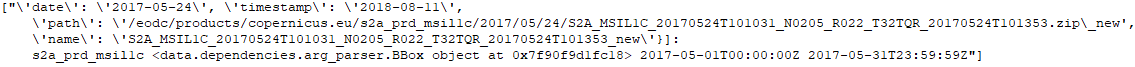
\includegraphics[width=\textwidth]{eva_data_changes_7_state}
	%	\caption{Step 1: State of the re-execution of pidA at the 7th evaluation step.}
	%	\label{fig:eva_data_changes_7_state} % \label has to be placed AFTER \caption (or \subcaption) to produce correct cross-references.
	%\end{figure}
	
	\begin{code}
		\begin{minted}[fontsize=\small]{text} 
[{'timestamp': '2019-03-31 17:44:43', 
'path': '/eodc/products/copernicus.eu/s2a_prd_msil1c/2017/05/24/
S2A_MSIL1C_20170524T101031_N0205_R022_T32TQR_20170524T101353_new.zip'}]
		\end{minted}
		\caption{List of files that replaced original files of the query result.}
		\label{lst:eva_datachange_state}
	\end{code}

	\item \textbf{Run duplicate of \textit{jobA}, by using the data PID of \textit{jobA} named \textit{jobD}}\\
	Listing \ref{lst:eva_datachange_8} shows the code of running a new \textit{jobD} with the data of \textit{pidA}. The code is executed after the deletion of one file from the resulting file list of \textit{pidA}. After the creation of the job, the backend notices that the number of result files is different than the first execution of the input data PID. Therefore, a warning message is displayed at the client of the researcher \bgoesswein{(see Listing \ref{lst:eva_datachange_8})}. If the user starts the job nevertheless, the backend looks for updated files like described in the previous step and adds the most recent version of the missing file to the query result. \bgoesswein{EODC chose this strategy, since updates on datasets usually fix errors, users expect the most recent ones. Most backends e.g. Google Earth Engine give the users the most recent version automatically.} The backend creates a new data PID for \textit{jobD}, since the query result changed. Table \ref{Tab:eva_datachanges5} shows the query table status after the execution. The second query entry has a different result hash, since one file changed. 
	\begin{code}
		\begin{minted}[fontsize=\small]{python}
# Take input data of job A by using the input data PID A of job A
pgD = processes.get_data_by_pid(data_pid=pidA)
# Choose processes
pgD = processes.ndvi(pgC, nir="B08", red="B04")
pgD = processes.min_time(pgD)
# Create and start Job D
jobD = con.create_job(pgD.graph)
# Stdout: Warning: The resulting file list changed from the original query
# execution! Look into the "diff" attribute to see the list of files that
# have changed. The original data might be still obtainable by the original data provider. Please contact the backend provider for further information. 
jobD.start_job()
pidD = jobD.get_data_pid() # pidD != pidA
		\end{minted}
		\caption{Run duplicate of \textit{jobA}, by using the data PID of \textit{jobA} named \textit{jobD}.}
		\label{lst:eva_datachange_8}
	\end{code}

	\begin{table}[]
		\caption{Query table after the execution of Listing \ref{lst:eva_datachange_4}. Important elements are highlighted blue if they are the same and red if they are different.}
		\centering
		\begin{tabular}{|r|l|}
			\hline \multicolumn{2}{|c|}{\textbf{Query \textit{pidA} (full entry in Table \ref{Tab:eva_datachanges1})}} \\
			\hline \multicolumn{1}{|c|}{\textbf{Column}}  &  \multicolumn{1}{c|}{\textbf{Value}} \\ \hline
			Query PID & {\color{red}qu-a3bbe4a0-a875-4687-bb78-9457f33134a9}  \\ 
			Unique Hash & {\color{blue}0917c7a21cec960b8a6617...}  \\
			Result Hash & {\color{red}abf43f519007050cbaeb59...}   \\
			Metadata & \{'result\_files': 51\}  \\
			\hline \multicolumn{2}{|c|}{\textbf{Query \textit{pidD}}} \\
			\hline \multicolumn{1}{|c|}{\textbf{Column}}  &  \multicolumn{1}{c|}{\textbf{Value}} \\ \hline
			Query PID & { \color{red} qu-3544aeae-cd24-4b6d-ad34-0d674c2a400f}  \\ 
			Dataset PID & s2a\_prd\_msil1c  \\ 
			Original Query & \textit{see Figure \ref{fig:appendix_pidD} in the appendix} \\
			Unique Query & \textit{see Listing \ref{lst:eva_datachange_nq1}}  \\
			Query Hash & {\color{blue}0917c7a21cec960b8a6617...}  \\
			Result Hash & {\color{red}28088d113de19ce037e965...}  \\
			Metadata & \{'result\_files': 51\}  \\
			Execution Timestamp & 2019-03-31 18:10:25.46402   \\ \hline
		\end{tabular}
		\label{Tab:eva_datachanges5}
	\end{table}
\end{enumerate}

The result of the second test case shows how the backend behaves on data updates replacing the original data. If the file is deleted, the researcher gets a warning message and a list of files that are replacing the original files. Since the path of the file identifies the date and tile that was used, the researcher can notify EODC about the concrete changed file. On creation of the new \textit{jobD} that uses the input data identifier \textit{pidA}, the client notifies the user that the result files changed, before the execution happens. Then the user can decide to start the job nevertheless or contact EODC about the modified files.

\subsection{Test Case 3: Is it possible to re-execute a query after a data file is deleted?}
The deletion of a file without a new file replacing it is not within the policies of EODC since it would restrict their range on available data. If it happens nevertheless, there is in the current solution no possibility to get the exact removed files. The number of result files in the "meta\_data" column shows how many files changed. The whole result files need to be added to the query table to achieve the knowledge of missing files. In our solution, the user has to notify EODC about the missing files. How EODC gets the files from ESA in such a case is not in scope of this thesis.

%EODC can then look up the files that were deleted using the filter arguments of the query to identify the original files and copy them from ESA. 

%The researcher can query the data at ESA directly with the same filter arguments and can compare the resulting file list with the ones from the re-execution of EODC, but the solution is not doing it automatically.  

%The remaining question is how the system behaves if the data is updated during the query processing. Since there is no permission to perform a test on it, it can only be assumed theoretically. Since the query system is file based and an update results in a new file replacing an existing file. There are two possibilities of the outcome of a query be executed at the same time. Either the query results in the old file, which then will result in an error at the execution if the file is replaced already at the time of the job execution, or the query results in the new file. In both cases the data PID will be generated consistent with the job execution, since it takes the original executed query and the actual file list used for the execution.     
\newpage
\section{Job Capturing}\label{Evaluation:special_jobcap}

This section reviews the capabilities of the solution regarding job capturing. The focus is on the context model of the job execution. The following question is used to discuss the impact of the captured data regarding job execution. \\

\textbf{Is it possible to recreate an older version of the backend?} \\
The solution aims to capture enough data to make it possible to re-run the same job at the same backend. The backend is created directly by its GitHub repository. The GitHub repository URL and the commit identifier of the original setup are needed to recreate an old version of the backend. The timestamp of the job execution is stored in the context model of the original job execution. The backend provenance can resolve the version of the backend and therefore the GitHub repository and commit via execution timestamp. Therefore, the information on re-creating a backend version from an older version is captured. The process graph of the job is persisted as well. The re-execution of the job is the same, assuming the input data has not been deleted in the meantime, which can be checked by re-executing the data query of the job. The resulting hash makes it possible to validate if the job re-execution us done in the same way. The following code presents how this can be achieved in our solution.

\begin{enumerate}
	\item \textbf{Run \textit{jobA}, which creates query \textit{pidA} and \textit{job\_idA}.} \\
	The first step shows the definition, creation, and execution of \textit{jobA}. The last two lines show the retrieval of the backend version. The "con.version()" method returns the current version of the backend, but can also take a timestamp as parameter to get the version of a particular time. The "jobA.get\_backend\_version()" method returns the version of the backend during the execution of \textit{jobA}. Both versions are at the end of Step 1 identical. 
	\begin{code}
		\begin{minted}[fontsize=\small]{python}
import openeo
# Connect with GEE backend
con = openeo.connect("http://openeo.local.127.0.0.1.nip.io")
# Choose dataset
processes = con.get_processes()
pgA = processes.get_collection(name="s2a_prd_msil1c")
pgA = processes.filter_daterange(pgA, extent=["2017-05-01", "2017-05-31"])
pgA = processes.filter_bbox(pgA, west=10.288696, south=45.935871, 
east=12.189331, north=46.905246, crs="EPSG:4326")
# Choose processes
pgA = processes.ndvi(pgA, nir="B08", red="B04")
pgA = processes.min_time(pgA)
# Create and start job A
jobA = con.create_job(pgA.graph)
jobA.start_job()
# Get current backend version
version_old = con.version()
# Get backend version of jobA 
versionA = jobA.get_backend_version()
		\end{minted}
		\caption{Step 1: Researcher runs \textit{jobA} and gets the used backend version.}
		\label{lst:eva_jobcapture_1}
	\end{code}
	
	\begin{code}
		\begin{minted}[fontsize=\small]{json}
{'branch': 'master',
'commit': '1a0cefd25c2a0fbb64a78cd9445c3c9314eaeb5b',
'url': 'https://github.com/bgoesswein/implementation_backend.git'}
		\end{minted}
		\caption{Step 1: Version of the \textit{jobA} execution \textit{version\_old}.}
		\label{lst:eva_jobcapture_1_1}
	\end{code} 

	\item \textbf{Publish \textit{job\_idA} and \textit{pidA}.} \\
	The researcher retrieves the persistent input data identifier \textit{pidA} and the job identifier \textit{jobA\_id} to cite the provenance of the execution. The timestamp of the execution in the context model is used to identify the backend version of the job execution.
	\begin{code}
		\begin{minted}[fontsize=\small]{python}
# Get input data PID of jobA 
pidA = jobA.get_data_pid()
jobA_id = jobA.job_id
		\end{minted}
		\caption{Researcher gets the input data PID of \textit{jobA} and the \textit{job\_id} of \textit{jobA}.}
		\label{lst:eva_jobcapture_2}
	\end{code}
	
	\item \textbf{Update backend version} \\
	In this step, we modify the backend by updating one Python package in the requirements file used for the job execution. We edit the file by replacing the line "urllib3==1.23" with "urllib3==1.24.1". After editing we call the "git commit" command to get a new version of the backend. 
	\item \textbf{Get original context of \textit{jobA}} \\
	Listing \ref{lst:eva_jobcapture_4} shows the code needed by the researcher to get the original version of the backend during the \textit{jobA} execution. The variable \textit{versionA} contains the version displayed in Listing \ref{lst:eva_jobcapture_1_1}. 
	\item \textbf{Re-run \textit{jobA} with the original version.} \\
	To get the original version of the backend, EODC has to create a second instance of the backend. Then they have to check out the commit of the job execution, by running "git checkout commit\_id" in the console, where "commit\_id" is the value of \textit{versionA["commit"]}.
	\begin{code}
		\begin{minted}[fontsize=\small]{python}
import openeo
# Connect with GEE backend
con = openeo.connect("http://openeo.local.127.0.0.1.nip.io")
# Get jobA using the jobA_id.
jobA = con.get_job(jobA_id)
# Get the version of the backend that was active during the job A execution
versionA = jobA.get_backend_version()
		\end{minted}
		\caption{Researcher retrieves the original backend version of the \textit{jobA} execution.}
		\label{lst:eva_jobcapture_4}
	\end{code}	
\end{enumerate}

\section{Performance and Storage Impact}\label{Evaluation:impact}

This section evaluates the performance and storage impact of the solution on the EODC backend. We define 18 input process graphs from 9 publications using data provided by EODC from the last two years. The data used in the papers provide spatial and temporal extents. These 18 input process graphs define the 18 test cases. Table \ref{Tab:appendix} shows the papers used for the test cases. The evaluation code (see evaluation\_impact.py on GitHub) contains the values of the spatial and temporal extent. The performance of the \textit{Solution Backend} is compared to a local EODC backend, without the extensions of this thesis (from now on referred to as \textit{Reference Backend}). Note that in the \textit{Reference Backend} the processing is mocked up in the same way as in the \textit{Solution Backend}. Figure \ref{fig:experiment_overview} gives an overview of the performance and storage evaluation setup.  

\begin{figure}[h]
	\centering
	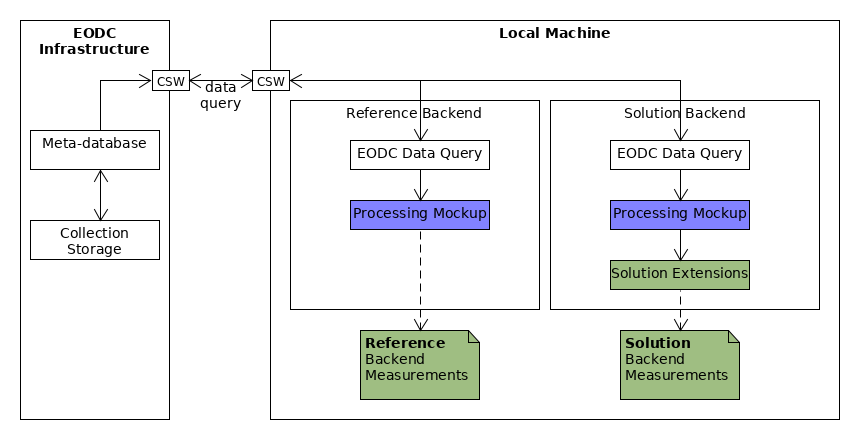
\includegraphics[scale=0.5]{experiment_overview}
	\caption{Overview of the storage and performance evaluation setup.}
	\label{fig:experiment_overview} % \label has to be placed AFTER \caption (or \subcaption) to produce correct cross-references.
\end{figure}

\begin{table}[]
	\caption{List of geoscientific papers used for the input data of the impact evaluation in Section \ref{Evaluation:Setup}}
	\centering
	\begin{tabular}{c|c|c}
		\textbf{Test Cases} & \textbf{DOI} & \textbf{Citation}  \\ \hline
		1 & 10.1080/01431160902887339 & \cite{evaluation1} \\ 
		2-4 & 10.3390/rs8050402 & \cite{evaluation2} \\ 
		5,6 & 10.1016/j.jag.2014.12.001  & \cite{evaluation3} \\
		7 & 10.1016/j.jag.2016.12.003  & \cite{evaluation4} \\
		8 & 10.3390/rs8110938  & \cite{evaluation5} \\
		9 & 10.1080/2150704X.2016.1225172  & \cite{evaluation6} \\
		10-13 & 10.1109/TGRS.2018.2858004  & \cite{evaluation7} \\
		14 & 10.1080/01431161.2018.1479788  & \cite{evaluation8} \\
		15-18 & 10.3390/rs10071030  & \cite{evaluation9} \\
	\end{tabular}
	\label{Tab:appendix}
\end{table}

\subsection{Performance}\label{Evaluation:impact_perf}

In this section, we evaluate the performance impact on the backend by measuring the difference of job execution durations between the \textit{Reference Backend} and the \textit{Solution Backend}. We measure the execution time by writing timestamps into a log file and calculating the duration afterward. We measure the duration of the \textit{Query Handler} (see Section \ref{Implementation:Data Identification}) execution, as well as the duration of the context model creation process (described in Section \ref{Implementation:Job dependent provenance}). Each test case is executed 50 times at each backend. Before the test case execution, we cleanup the backend, so that every iteration has the same backend condition. 

\subsubsection{Performance of Query Handler}\label{Evaluation:impact_perf_query}
This section provides a description regarding performance constraints for each element of the query table.

\begin{itemize}
	\item \textbf{Dataset PID} \\
	We take the \textit{Dataset PID} directly from the parsed filter arguments of the backend. Therefore, the duration has a complexity of $O(1)$. Figure \ref{fig:evaluation_perf_datapid} shows the performance results, which are between 4 µs and 26 µs with a median of 8 µs. the standard deviation over all test cases is 2.5 µs. The results show that the duration time of retrieving the dataset PID is, except for a few aberrations, similar between all test case executions and independent of the job configuration.
	\begin{figure}[!h]
		\centering
		\caption{Boxplot of the duration needed in the test cases to handle the \textit{Dataset PID} entry. }
		\label{fig:evaluation_perf_datapid}
		\begin{tikzpicture}
		\begin{axis}
		[
		xlabel={duration [µs]},
		y=2cm,
		ytick={1},
		yticklabels={Dataset PID},
		]
		\addplot+[
		boxplot prepared={
			lower whisker=4,
			lower quartile=6,
			median=8,
			upper quartile=9,
			upper whisker=26,
			box extend=1,
			whisker extend=0.5,
		},
		] coordinates {};
		\end{axis}
		\end{tikzpicture}
	\end{figure}

	\item \textbf{Original Query} \\
	The \textit{Query Execution} component passes the \textit{Original Query}. The \textit{Query Handler} transforms the query into a string. The query string has the same size for each query, and just the argument values are exchanged. Therefore the duration has a complexity of $O(1)$. The execution time of the test cases is between 24 µs and 98 µs, with a median of 37 µs. The standard deviation for all test cases is 5.34 µs. Figure \ref{fig:evaluation_perf_original} shows the boxplot of all test case executions and therefore the distribution of duration. The measurements indicate that most of the \textit{Original Query} retrieval time is in a small range. The duration of \bgoesswein{retrieving the original query} is constant in time and independent on the job configuration. 
	\begin{figure}[!h]
		\centering
		\caption{Duration boxplot of the test cases to handle the \textit{Original Query} entry.}
		\label{fig:evaluation_perf_original}
		\begin{tikzpicture}
		\begin{axis}
		[
		xlabel={duration [µs]},
		y=2cm,
		ytick={1},
		yticklabels={Original Query},
		]
		\addplot+[
		boxplot prepared={
			lower whisker=24,
			lower quartile=29,
			median=37,
			upper quartile=45,
			upper whisker=98,
			box extend=1,
			whisker extend=0.5,
		},
		] coordinates {};
		\end{axis}
		\end{tikzpicture}
	\end{figure}

	\item \textbf{Unique Query} \\
	The \textit{Unique Query} is the result of an alphabetical sorting of the parsed filter arguments of the backend. It takes nearly constant duration time, since there are only 4 filter arguments allowed in the openEO API version 0.3.1, but they may not all be used. The sorting algorithm has a complexity of $O(n\log{}n)$, where "n" is the number of crucial elements in the dictionary (amount of filter operations). In this evaluation, four filter arguments were used for each test case. Therefore it has a constant complexity in every test case execution. It takes between 38 µs and 132 µs with a median of 59 µs of duration time with a standard deviation of 19.35 µs. Figure \ref{fig:evaluation_perf_normalized} shows the boxplot of all test case executions to visualize that the duration is not widely distributed.  
	\begin{figure}[!h]
		\centering
		\caption{Boxplot of the duration time of the test cases to handle the \textit{Unique Query} entry.}
		\label{fig:evaluation_perf_normalized}
		\begin{tikzpicture}
		\begin{axis}
		[
		xlabel={duration [µs]},
		y=2cm,
		ytick={1},
		yticklabels={Unique Query},
		]
		\addplot+[
		boxplot prepared={
			lower whisker=38,
			lower quartile=47,
			median=59,
			upper quartile=75,
			upper whisker=132,
			box extend=1,
			whisker extend=0.5,
		},
		] coordinates {};
		\end{axis}
		\end{tikzpicture}
	\end{figure}

	\item \textbf{Query Hash} \\
	The performance of the unique \textit{Query Hash} is dependent on the size of the unique query ($O(n)$, where "n" is the size of the unique query string). In this evaluation, it is constant because every test case uses four filter arguments. The circumstances makes the unique query have a constant length. In the test cases, the duration is between 15 µs and 54 µs with a median of 20 µs and a standard deviation of 5.89 µs. Figure \ref{fig:evaluation_perf_norm_hash} shows the boxplot of all test case executions. The duration has a small range of distribution, except for a few executions. The measurements show that the duration is independent of the job configuration. 
	\begin{figure}[!h]
		\centering
		\caption{Boxplot of the duration time of the test cases to handle the \textit{Query Hash} entry.}
		\label{fig:evaluation_perf_norm_hash}
		\begin{tikzpicture}
		\begin{axis}
		[
		xlabel={duration [µs]},
		y=2cm,
		ytick={1},
		yticklabels={Query Hash},
		]
		\addplot+[
		boxplot prepared={
			lower whisker=15,
			lower quartile=17,
			median=20,
			upper quartile=25,
			upper whisker=54,
			box extend=1,
			whisker extend=0.5,
		},
		] coordinates {};
		\end{axis}
		\end{tikzpicture}
	\end{figure}

	\item \textbf{Result Hash} \\
	Duration of the \textit{Result Hash} creation is dependent on the length of the result file list. The SHA-256 operation has a complexity of $O(n)$, where "n" is the length of the resulting file list string. In the test cases, the duration time of the \textit{Result Hash} calculation is between 28 µs and 9167 µs with a median of 51 µs. Figure \ref{fig:evaluation_data_resulthash} shows the duration of the \textit{Result Hash} creation of the test cases, sorted by the size of the result file set in an ascending way. Table \ref{Tab:data_result_hash} shows the values of the chart. They indicate the relationship between the number of files and the duration.  
	
	\begin{table}[]
		\caption{\textit{Result Hash} performance of the test cases depending on the number of result files.}
		
		\centering
		\begin{tabular}{c|c|c}
			\textbf{Test Case} & \textbf{Number of files} & \textbf{\textit{Result Hash} duration [µs]}  \\ \hline
			1 & 14  & 47.2 \\ \hline 
			2 & 24 & 78.0 \\ \hline
			3 & 11 & 37.2 \\ \hline
			4 & 9 & 32.4 \\ \hline
			5 & 10 & 35.0 \\ \hline
			6 & 10 & 35.9 \\ \hline
			7 & 10 & 33.8 \\ \hline
			8 & 12 & 36.9 \\ \hline
			9 & 2255 & 8698.7 \\ \hline
			10 & 17 & 59.4 \\ \hline
			11 & 1551 & 5343.9 \\ \hline
			12 & 12 & 41.5 \\ \hline
			13 & 28 & 95.2 \\ \hline
			14 & 420 & 1400.7 \\ \hline
			15 & 15 & 50.1 \\ \hline
			16 & 1356 & 4985.0 \\ \hline
			17 & 15 & 51.6 \\ \hline
			18 & 54 & 187.2 \\ 
		\end{tabular}
		\label{Tab:data_result_hash}
	\end{table}
	
	\begin{figure}[h]
		\centering
		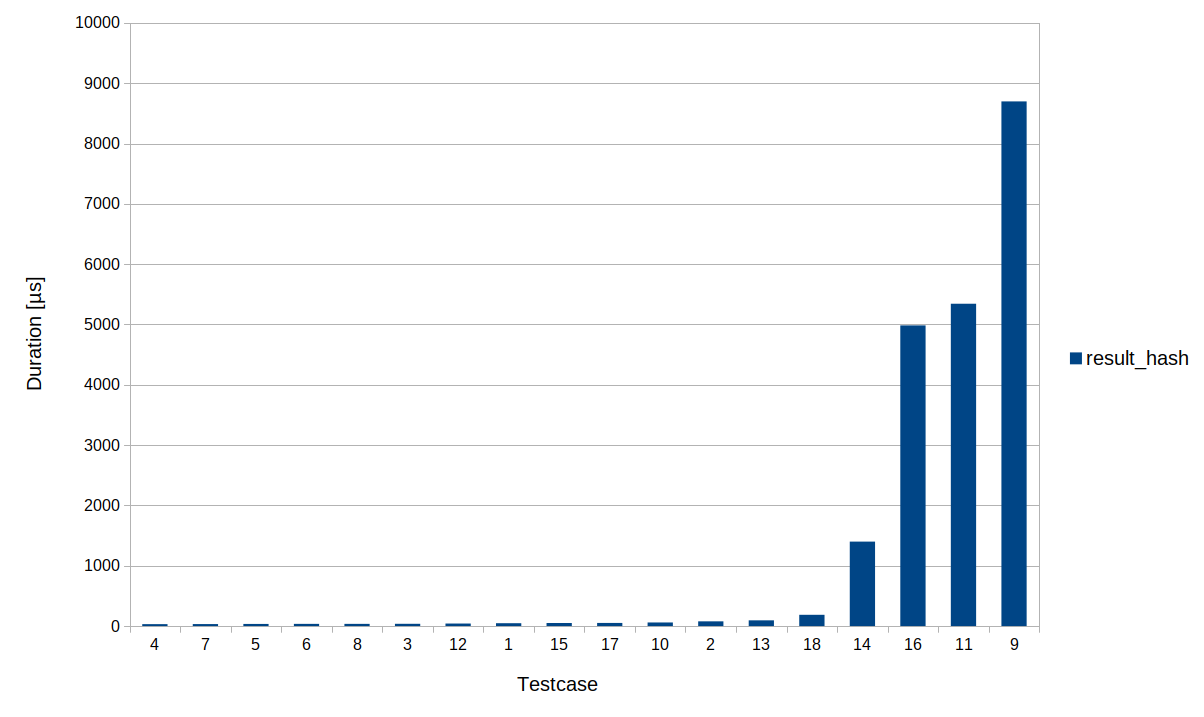
\includegraphics[scale=0.45]{eva_data_resulthash}
		\caption{\textit{Result Hash} duration of the test cases sorted by result size.}
		\label{fig:evaluation_data_resulthash} % \label has to be placed AFTER \caption (or \subcaption) to produce correct cross-references.
	\end{figure}
	
	%	\begin{figure}[h]
	%		\centering
	%		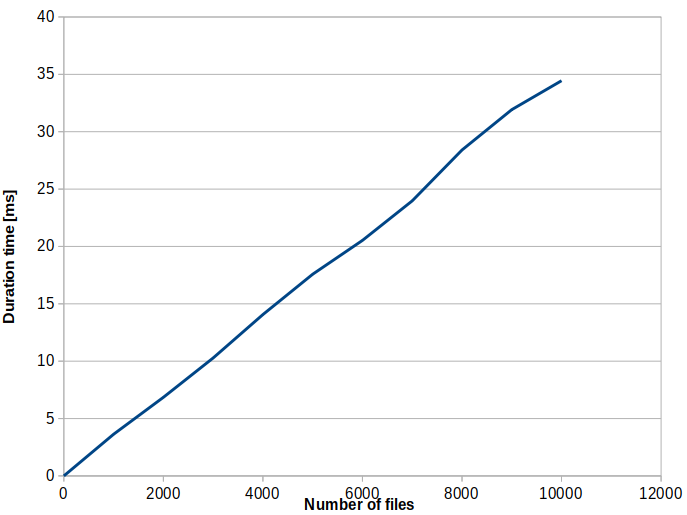
\includegraphics[scale=0.35]{evaluation_impact_data_resulthash}
	%		\caption{Execution duration of the sha-256 over the test cases.}
	%		\label{fig:evaluation_impact_data_resulthash} % \label has to be placed AFTER \caption (or \subcaption) to produce correct cross-references.
	%	\end{figure}

	\item \textbf{Metadata} \\
	In the solution the \textit{Metadata} contains only the number of result files. It measures it by the built-in len() operator of Python, which has a complexity of $O(1)$ according to the official Python description\footnote{https://wiki.python.org/moin/TimeComplexity}. In the test cases, the data calculation takes a duration between 6 µs and 359 µs with a median of 12 µs and a standard deviation of 3.98 µs. Figure \ref{fig:evaluation_perf_meta_data} shows the boxplot of the test case execution. The measurements indicate no correlation of the test case configuration and the duration.
	\begin{figure}[!h]
		\centering
		\caption{Boxplot of the duration time of the test cases to handle the \textit{Metadata} entry.}
		\label{fig:evaluation_perf_meta_data}	
		\begin{tikzpicture}
		\begin{axis}
		[
		xlabel={duration [µs]},
		y=2cm,
		ytick={1},
		yticklabels={Metadata},
		]
		\addplot+[
		boxplot prepared={
			lower whisker=6,
			lower quartile=10,
			median=12,
			upper quartile=17,
			upper whisker=359,
			box extend=1,
			whisker extend=0.5,
		},
		] coordinates {};
		\end{axis}
		\end{tikzpicture}
	\end{figure}
	
	\item \textbf{Database operations} \\
	To ensure that there are no duplicate query entries in the database, the \textit{Query Handler} executes a SQL SELECT statement to check if there is already an entry with the same unique query hash and the same result hash. In the evaluation, the query table is empty before the SELECT statement. Hence, the complexity is $O(1)$. \bgoesswein{There is currently no statistic of queries at EODC, but an estimation of a few hundred per month.} The INSERT statement to store the query has a complexity of $O(1)$. The database operations in the test cases have a duration between 10.501 ms and 49.283 ms with a median of 13.377 ms. Figure \ref{fig:evaluation_perf_data_database} shows the boxplot of the test case executions indicating that the performance is independent of the job configuration.  
	\begin{figure}[!h]
		\centering
		\caption{Boxplot of the duration time of the test cases to make the needed database operations.}
		\label{fig:evaluation_perf_data_database}	
		\begin{tikzpicture}
		\begin{axis}
		[
		xlabel={duration [ms]},
		y=2cm,
		ytick={1},
		yticklabels={database operations},
		]
		\addplot+[
		boxplot prepared={
			lower whisker=10.501,
			lower quartile=11.837,
			median=13.377,
			upper quartile=16.680,
			upper whisker=49.283,
			box extend=1,
			whisker extend=0.5,
		},
		] coordinates {};
		\end{axis}
		\end{tikzpicture}
	\end{figure}
\end{itemize}

Figure \ref{fig:eva_data_static} shows the duration of the constant query elements of the test cases. The test cases are sorted by the result size in ascending order. It shows that even though we configured the test cases differently, the duration time of the constant query elements are similar between them. 

\begin{figure}[h]
	\centering
	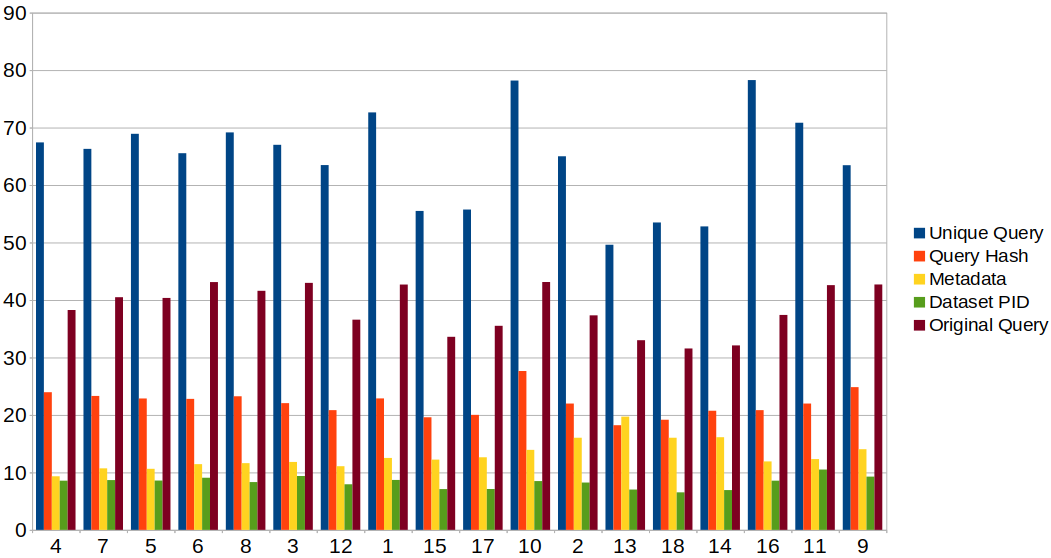
\includegraphics[scale=0.55]{eva_data_static}
	\caption{Constant elements of the \textit{Query Handler} output in relation to the test cases sorted by result size.}
	\label{fig:eva_data_static} % \label has to be placed AFTER \caption (or \subcaption) to produce correct cross-references.
\end{figure}


\subsubsection{Performance of Context Model Creation}\label{Evaluation:impact_perf_context}

\begin{enumerate}
	\item \textbf{Constant context model elements} \\
	The creation of the following elements of the context model have a constant duration: 
	\begin{itemize}
		\item The programming language
		\item The input data identifier
		\item The backend version
		\item The start and end timestamp
	\end{itemize}
	These are independent of the job configuration and are read operations with a complexity of $O(1)$. The constant context model elements in the test cases have a duration between 26 µs and 122 µs with a median of 41.5 µs. Figure \ref{fig:evaluation_perf_static_cm} shows the boxplot of the test case executions to visualize the distribution.
	\begin{figure}[!h]
		\centering
		\caption{Boxplot of the duration time of the test cases to handle the constant context model elements.}
		\label{fig:evaluation_perf_static_cm}		
		\begin{tikzpicture}
		\begin{axis}
		[
		xlabel={duration [µs]},
		y=2cm,
		ytick={1},
		yticklabels={Constant Elements},
		]
		\addplot+[
		boxplot prepared={
			lower whisker=26,
			lower quartile=34,
			median=41.5,
			upper quartile=47,
			upper whisker=122,
			box extend=1,
			whisker extend=0.5,
		},
		] coordinates {};
		\end{axis}
		\end{tikzpicture} 
	\end{figure}

	\item \textbf{Dependencies of the programming language} \\
	A "pip freeze" execution retrieves the dependencies of the backend. It is independent on the complexity of the job, hence has a constant duration time. The duration in the test cases executions is between 92 µs and 289 µs with a median of 133 µs. Figure \ref{fig:evaluation_perf_python} shows the boxplot of the test case execution to visualize the distribution.
	\begin{figure}[!h]
		\centering
		\caption{Boxplot of the duration time of the test cases to retrieve the modules of Python.}
		\label{fig:evaluation_perf_python}		
		\begin{tikzpicture}
		\begin{axis}
		[
		xlabel={duration [µs]},
		y=2cm,
		ytick={1},
		yticklabels={python modules},
		]
		\addplot+[
		boxplot prepared={
			lower whisker=92,
			lower quartile=112,
			median=133,
			upper quartile=150.5,
			upper whisker=289,
			box extend=1,
			whisker extend=0.5,
		},
		] coordinates {};
		\end{axis}
		\end{tikzpicture}
	\end{figure}

	\item \textbf{Result hash} \\
	The duration of the resulting hash calculation is dependent on the length of the resulting image. The SHA-256 operation has a complexity of $O(n)$, where "n" is the size of the output image. In the test cases, the duration is between 1.924 ms and 106.270 ms with a median of 2.521 ms. Table \ref{Tab:result_hash} shows the test cases and their result size concerning the average duration time of the result hash calculation. In the experiment setup, every 100 kByte of output data resulted in average in an additional duration of 371 µs. The test cases 9, 11, 14, and 16 have the most prominent result file and therefore needed the longest for the result hash calculation.     
	
	\begin{table}[]
		\centering
		\caption{Result hash performance of the test cases in relation to the result size.}
		\begin{tabular}{c|c|c}
			\textbf{Test Case} & \textbf{Result size [kByte]} & \textbf{Result hash duration [ms]}  \\ \hline
			1 & 587  & 2.2 \\ \hline 
			2 & 721 & 2.7 \\ \hline
			3 & 600 & 2.2 \\ \hline
			4 & 556 & 2.1 \\ \hline
			5 & 570 & 2.1 \\ \hline
			6 & 553 & 2.1 \\ \hline
			7 & 578 & 2.1 \\ \hline
			8 & 638 & 2.4 \\ \hline
			9 & 27 999 & 104.2 \\ \hline
			10 & 621 & 2.3 \\ \hline
			11 & 7 969 & 29.7 \\ \hline
			12 & 649 & 2.4 \\ \hline
			13 & 1 376 & 5.1 \\ \hline
			14 & 6 026 & 22.4 \\ \hline
			15 & 777 & 2.9 \\ \hline
			16 & 7 978 & 29.7 \\ \hline
			17 & 733 & 2.7 \\ \hline
			18 & 706 & 2.6 \\ 
		\end{tabular}
		\label{Tab:result_hash}
	\end{table}

	\item \textbf{Database UPDATE operation} \\
	The job entry gets updated to store the context model in the database by a SQL UPDATE statement. It is independent of the job configuration. The duration of the test case execution is between 3.631 ms and 20.099 ms, with a median of 5.493 ms. Figure \ref{fig:evaluation_perf_database} shows the boxplot of the test case execution to visualize the distribution. 
	
	\begin{figure}[!h]
		\centering
		\caption{Boxplot of the duration time of the test cases to retrieve the modules of Python.}
		\label{fig:evaluation_perf_database}		
		\begin{tikzpicture}
		\begin{axis}
		[
		xlabel={duration [ms]},
		y=2cm,
		ytick={1},
		yticklabels={UPDATE operation},
		]
		\addplot+[
		boxplot prepared={
			lower whisker=3.631,
			lower quartile=4.595,
			median=5.493,
			upper quartile=7.237,
			upper whisker=20.099,
			box extend=1,
			whisker extend=0.5,
		},
		] coordinates {};
		\end{axis}
		\end{tikzpicture}
	\end{figure}
	
\end{enumerate}

The context model creation performance is not affected by the complexity of the test cases. The captured data for the context model is not related to the complexity of the job execution. The "Increase" column of Table \ref{Tab:eva_performance} shows that simple test cases are affected the most in terms of relative performance loss because the \textit{Query Handler} and the context model have elements that need the same execution duration. In conclusion, it can be argued that the execution of the \textit{Query Handler} and the context model creation is less affecting complex test cases, \bgoesswein{because of the constant overhead, which adds a fixed amount of time}. Besides, it should be mentioned that the \textit{Query Handler} and the context model creation happens after the processing. So that the result files of the job execution are available for the user even if both modules have not finished yet. \\
Table \ref{Tab:eva_performance} summarizes the result of the mean duration time over the 50 runs of each the test case. The second column presents the duration of the \textit{Reference Backend}. The other columns are measurements of the \textit{Solution Backend}. It includes the total execution duration of the \textit{Solution Backend}, the duration of the \textit{Query Handler} and the duration of the context model creation. The last column shows the additional time the \textit{Solution Backend} needs in comparison to the \textit{Reference Backend}. The last row of Table \ref{Tab:eva_performance} shows the mean duration over all test cases. It indicates that the solution adds between 20 ms and 175 ms to the duration of the \textit{Reference Backend}. It depends on the result sizes and not on the execution duration of the job execution. Compared to the estimated computation time of the test cases between 10 seconds and 20 minutes at the production version of the EODC backend, we conclude that the impact of the \textit{Query Handler} is negligible.

\begin{table}[]
	\caption{Mean duration time over 50 runs of the \textit{Solution Backend} and the \textit{Reference Backend} by executing the test cases}
	\begin{tabular}{r|r|r|r|r|r}
		
		\textbf{} & \textbf{Reference Backend} & \multicolumn{3}{c|}{\textbf{Solution Backend}} &  \\ \hline \textbf{Test} & \textbf{} & \textbf{Comparison} & \textbf{Query} & \textbf{Context} & \textbf{Solution} \\ 
		\textbf{Case} & \textbf{Total} & \textbf{Total} & \textbf{Handler} & \textbf{Model} & \textbf{Addition} \\ \hline
		1 & 322.946 ms & 345.127 ms & 14.187 ms & 7.994 ms & 22.181 ms (6.8 \%) \\ 
		2 & 369.066 ms & 393.505 ms & 16.342 ms & 8.097 ms & 24.439 ms (6.6 \%)\\ 
		3 & 281.657 ms & 305.407 ms & 15.669 ms & 8.081 ms & 23.750 ms (8.4 \%)\\ 
		4 & 276.324 ms & 298.954 ms & 14.015 ms & 8.615 ms & 22.630 ms (8.2 \%)\\ 
		5 & 312.150 ms & 334.802 ms & 13.925 ms & 8.727 ms & 22.652 ms (7.3 \%)\\ 
		6 & 314.571 ms & 337.290 ms & 13.985 ms & 8.734 ms & 22.719 ms (7.2 \%)\\ 
		7 & 320.081 ms & 343.552 ms & 14.555 ms & 8.916 ms & 23.471 ms (7.3 \%)\\ 
		8 & 304.998 ms & 328.633 ms & 14.742 ms & 8.893 ms & 23.635 ms (7.7 \%)\\ 
		9 & 565.289 ms & 740.751 ms & 48.766 ms & 126.696 ms & 175.462 ms (31.0 \%)\\ 
		10 & 401.922 ms & 425.026 ms & 14.874 ms & 8.230 ms & 23.104 ms (5.7 \%)\\ 
		11 & 521.022 ms & 605.185 ms & 34.660 ms & 49.503 ms & 84.163 ms (16.2 \%)\\ 
		12 & 387.536 ms & 412.079 ms & 15.711 ms & 8.832 ms & 24.543 ms (6.3 \%)\\ 
		13 & 510.517 ms & 538.784 ms & 17.070 ms & 11.197 ms & 28.267 ms (5.5 \%)\\ 
		14 & 657.989 ms & 706.329 ms & 19.010 ms & 29.330 ms & 48.340 ms (7.3 \%)\\ 
		15 & 345.806 ms & 371.984 ms & 17.027 ms & 9.151 ms & 26.178 ms (7.6 \%)\\ 
		16 & 585.730 ms & 658.493 ms & 23.956 ms & 48.807 ms & 72.763 ms (12.4 \%)\\ 
		17 & 563.755 ms & 589.776 ms & 16.778 ms & 9.243 ms & 26.021 ms (4.6 \%)\\ 
		18 & 836.377 ms & 862.271 ms & 16.801 ms & 9.093 ms & 25.894 ms (3.1 \%)\\ \hline
		\textbf{Avg.} & \textbf{437.652 ms} & \textbf{477.664 ms} & \textbf{19.004 ms} & \textbf{21.008 ms} & \textbf{40.012 ms (8.9 \%)} \\ 
	\end{tabular}
	\label{Tab:eva_performance}
\end{table}

% The result hash is the only element that is dependent on the complexity of the test case. Most of the complexity comes from the temporal extent of the test cases, which do not affect the size of the resulting file. The reason for this is that the output file is always a composite of the values throughout the time range.
\newpage
\subsection*{Storage}\label{Evaluation:impact_stor}

This section describes the storage needed for the captured data. The \textit{Solution Backend} stores all of the captured data in a PostgreSQL database. Therefore, we estimate the needed storage using the PostgreSQL command line interface. Listing \ref{lst:eva_imact_1} presents the commands to retrieve the size of the database entries. The id of the data record is inserted into "''" (e.g. job id in the first one).  

\begin{listing}[ht]
	\begin{minted}[fontsize=\small]{sql}
-- Context Model 
SELECT sum(pg_column_size(context_model)) as filesize, count(*) as filerow 
FROM jobs as t WHERE id = '{}';
-- Query Table
SELECT sum(pg_column_size(t)) as filesize, count(*) as filerow 
FROM query as t WHERE query_pid = '{}';
-- QueryJob Table
SELECT sum(pg_column_size(t)) as filesize, count(*) as filerow 
FROM queryjob as t WHERE job_id = '{}';
	\end{minted}
	\caption{PostgreSQL commands to retrieve the size of one data record in the job table, the query table and the queryjob table.}
	\label{lst:eva_imact_1}
\end{listing}	

%\begin{table}[]
%\caption{Mean storage over 50 runs of the solution by executing the test cases. All measured %values are in Bytes.}
%\centering
%\begin{tabular}{r|r|r|r|r}

%\textbf{Test Case} & \textbf{Context Model} & \textbf{Query} & \textbf{QueryJob} & \textbf{Sum}
%\\ \hline
%		1 & 1043 & 1529.659 & 113 & 2685.659 \\ 
%		2 & 1043 & 1530.583 & 113 & 2686.583 \\ 
%		3 & 1043 & 1525.585 & 113 & 2681.585 \\ 
%		4 & 1043 & 1533.649 & 113 & 2689.649 \\ 
%		5 & 1043 & 1524.622 & 113 & 2680.622 \\ 
%		6 & 1043 & 1520.267 & 113 & 2676.267 \\ 
%		7 & 1043 & 1524.800 & 113 & 2680.800 \\ 
%		8 & 1043 & 1527.614 & 113 & 2683.614 \\ 
%		9 & 1043 & 1532.814 & 113 & 2688.814 \\ 
%		10 & 1043 & 1523.184 & 113 & 2679.184 \\ 
%		11 & 1043 & 1530.667 & 113 & 2686.667 \\ 
%		12 & 1043 & 1524.825 & 113 & 2680.825 \\ 
%		13 & 1043 & 1529.923 & 113 & 2685.923 \\ 
%		14 & 1043 & 1525.614 & 113 & 2681.614 \\ 
%		15 & 1043 & 1524.683 & 113 & 2680.683 \\ 
%		16 & 1043 & 1530.422 & 113 & 2686.422 \\ 
%		17 & 1043 & 1524.846 & 113 & 2680.846 \\ 
%		18 & 1043 & 1521.432 & 113 & 2677.432 \\ \hline
%		\textbf{All} & \textbf{1043} & \textbf{1526.955} & \textbf{113} & \textbf{2682.955} \\
%	\end{tabular}
%	\label{Tab:eva_storage}
%\end{table}

The storage need for the evaluation is constant. The mean storage of the 50 runs per test case and the average storage size of the test cases are measured. Three parts of the implementation are storing data in the database. First, we store the context model in an additional column named "context\_model" in the job table. There is no element in the context model that can vary in size, except for the list of packages of Python, which didn't change during the evaluation. It takes an additional 1.043 kByte of size for every job entry. The same occurs at the queryjob table, which maps the query table and the job table and therefore contains the needed identifiers and timestamps for creation and modification. Every record of the queryjob table needs 0.113 kBytes of storage space.
The query records have a varying size because of the string length of the parameters in the original query. The remaining parts of the query table are constant in storage usage. Each query record of the test cases needs between 1.520 kByte and 1.533 kByte of space. The original query makes up the biggest part in the query table (e.g. 959 Bytes of 1521.432 Bytes in test case 18). The reason for this is the high amount of XML annotations. In summary, the average additional storage needed by the \textit{Solution Backend} per job with a new query entry is 2.677 kBytes. If the used query is already in the query table, only additional 1.043 kBytes are needed by the \textit{Solution Backend}. \bgoesswein{For EODC this are eligible numbers with the estimate of under one hundred queries and job executions.}
\newpage
\section{Summary}
The evaluation in this chapter showed how the solution tackles the goals of the research questions. First, it summarizes how the RDA recommendations are implemented in the solution, except for the migration recommendations (R14 and R15). The data identification implementation is then tested against exceptional test cases regarding data updates and data deletions at the backend. The evaluation shows that the solution can re-execute queries properly by returning old versions of updated files. The test cases show that the usage of the data PID as input data of a new job is superior to the current way of re-executing a job with the same process graph at EODC.
The reason for this is that the process graph does not have the original execution timestamp and therefore, does not use the same input data after an update occurs. In the evaluation of deleted data at the backend, the solution happens to be not capable of showing the exact missing files, since not the whole file list result of the query is persisted. The test case on job capturing showed that the solution is capable of identifying the backend version and therefore, the environment of the job execution. Still, to run a new job in the same environment, EODC has to provide it manually. The evaluation also contains a section about the performance and storage impact on the EODC backend, by running 18 test cases derived from past publications that used data from EODC. The results show that, except for the result hashes, the calculation of the data identification and the context model are independent of the complexity of the job. The time of the result hashing used for the data identification is dependent on the size of the query result, and the resulting hash of the context model is dependent on the size of the output file of the job execution. The evaluation of storage impact results in the conclusion that the additional needed space per job is unrelated to the job configuration. It depends on if there is a new query entry added to the database or not. The performance impact of the test case execution is between 20ms and 170ms. Compared to the estimated computation time of the test cases between 10 seconds and 20 minutes at the production version of the EODC backend, we conclude that the impact of the Query Handler is negligible. The additional needed space per job is constant and also minimal if compared to size of data kept at the backend.
   
\chapter{Conclusion and Future Work}\label{Conclusion}

\section{Conclusion}
%\todo{Always "the backend" not "the EODC backend", just in the first mentioning of the section}
%\todo{Remove automated fashion or add a Why? --> Because EODC does not provide a possibility or it has to be done manually by EODC}

In this thesis, the challenges of providing reproducibility in earth observation science have been explored. We dealt with the problematic state of reproducibility in EO experiments, which use extern computational backends. We suggested how existing infrastructure of EO backends can be adapted to enable data identification using the Research Data Alliance recommendations. We presented how job environments can be captured and compared, by applying the VFramework to make differences in the computational environment measurable. The presented solution was implemented at the backend of the Earth Observation Data Centre which is compliant with the openEO specification that provides a common interface for earth observation backends. The implementation involved extending the backend to add reproducibility supporting functionality, as well as, extending client applications to provide additional functionality. This allows scientists not to change the way of work but, due to the introduced changes into the existing environment, they can improve the reproducibility of experiments. The evaluation of our solution consists of simulated use cases representing updates of data and changes in the backend environment. We also measured the performance and storage impact on the backend, which concluded that the solution is capable of making the input data, code and the environment identifiable and reproducible with minimal impact on the backend's performance.       
\newpage
\subsection{Research questions revisited}\label{research question revisited}
%\todo{Update changed RQs !}
%\todo{Programming language --> programming language version}
%\todo{Redundante Sätze wegstreichen}
%\todo{first execution --> original execution}
%\todo{Remove "can assumed"}
%\todo{data compared --> Data ID or it changes to Context model somehow} --> REMOVED
This section revisits the research questions defined in Section \ref{research question} to discuss how the solution suits them.

\begin{itemize}
	\item \textbf{What information must be captured from an earth observation backend, so that a job execution can be repeated like the original execution?}
	\begin{itemize}
		\item \textbf{How can the data of the original execution be identified?} \\
		\bgoesswe{The data of an EO job execution is defined by a list of satellite images needed to execute the job. It it is specified by the satellite identifier and the filter operations of the job, which result in a backend specific query (e.g. CSW). We made it} identifiable by storing the original query following the RDA recommendations. Therefore, we assigned a persistent identifier to every unique query and result combination. We defined the result as the hash value of the resulting file list of the query execution. The landing page of the resolvable input data PID is a human-readable and machine-readable website. \bgoesswe{We extended the openEO API specification to access the information of the landing page using an openEO client application.}
		\item \textbf{How can the environment of the original execution be reproduced?} \\
		The original environment consists of the \bgoesswe{executed} code, the version of programming language, and the installed libraries. We use Git and GitHub in our implementation to identify a version of the backend. \bgoesswe{Each commit represents a version of code.} \bgoesswe{The version of the programming language as well as the installed libraries are captured during the execution of the job \bgoessweindel{using}. In our implementation we used the Python tool pip. The context model stores the three elements of the environment during the job execution.} The backend has to jump back to the version of the backend used during the job execution to reproduce the original execution environment.       
		\item \textbf{Which parts of the backend need to be extended?} \\
		The RDA recommendations have to be implemented at the query execution component of the backend. To realize the backend version, we recommend to use a version control system. The job execution environment has to be modified to capture the job dependent environment. After the execution of the job finished, we added the creation of a result hash. We suggest an additional database table to store the context model for every job.
		\item \textbf{How can the result of a re-execution in future environments be verified?} \\
		The solution contains a hash of the resulting output file. The user compares the result hash value of the re-execution with the original execution output hash to see if the result differs. \bgoesswe{If the result hash differs in a re-execution, the user is able to investigate which parts of the job environment may caused the inequality.}
	\end{itemize}
\newpage
	\item \textbf{What information must be persisted to enable validation of a job re-execution on \bgoesswe{an} earth observation backend?}
	\begin{itemize}
		\item \textbf{What are the validation requirements?} \\
		We defined the validation requirements as the equality of the captured data in the context model. We proposed the equality of the input data identifier, the execution environment and the hash of the output for validation,\bgoesswe{because they define the job execution comprehensively. If any of these parts are different in a re-execution, we conclude that the way the execution happened is different from the original one.}
		%\item \textbf{How can the data be compared?} \\
		%The data is compared to the equality of all components of the context model. Every item of the context model is compared with the same item of the re-execution context model. There are only three states at the comparison defined: "EQUAL" or the difference of the context model element.
		%\item \textbf{How can changes of input data at the backend be recognized?} \\
		%Our solution follows the RDA recommendation for the identification of input data. If the same query results in a different outcome, the backend creates a new input data identifier. 
		%By using the original data PID for the re-execution, the backend uses the original data. If there are irreversible changes at the original data, it is detected by the solution.
		\item \bgoesswe{REMOVED SECOND POINT DUE TO REDUNDANCY}  
		\item \textbf{How can differences in the environment between the executions be discovered?} \\
		The solution contains a user service to compare two job executions. It compares the context models of the two jobs and returns the differences. If a backend environment changes between two executions, the backend version is different.
	\end{itemize}
\end{itemize}

\section{Future Work}\label{FutureWork}
%\todo{improved --> customized}
%\todo{be positive about it, so show what can be improved rather than show that is not working yet...}
The prototype of this thesis applies reproducibility using a file-based openEO compliant backend. The openEO project is an ongoing project, hence the common API may evolve and our work will have to be adapted to new releases of the API. User defined functions (UDF) are part of the project, but not well defined yet. The extension of the design to support reproducible UDFs is a useful extension of the solution. Future work will lead to the implementation of the proposed solution at other backends of the openEO consortium. Further, the solution will be applied to backends that are not openEO compliant. Future effort will go into differently structured backends e.g. backends with non-file-based result sets. In the solution of this thesis, we capture environment information to identify how jobs are executed. \bgoesswe{Jobs are represented by the process graph and therefore, a compilation of single processes. Future work will improve the provenance of process implementations at the backend by introducing process versions. This will improve the transparency for users by enabling the identification of updated process implementations that may cause different results in a re-execution.}

%A finer granularity of the job capturing is a possible addition to the solution, leading to a definition of scalability. The granularity of the capturing can be customized to make the comparison of different execution behaviors more informative. This can lead to a context model of every executed process part of a job. The context model of the job in this example is a composite of the process execution context models. 

%\subsection{Benchmarking Mode}\label{Job:Benchmarking}

%So far, only the capturing of the whole process chain, including input and output data, are described. The general idea (presented in Section \ref{Implementation:Job dependent provenance}) of the job dependent provenance capturing is to capture the input data of the process graph, the whole process graph and the output of the process graph. It is a universal concept the backend providers can agree on since it is not affecting the backend providers implementations much. Moreover, it is capable of giving the user a simple overview of how the results are generated and what the differences between job executions are. The granularity of the capturing can be improved to make the comparison of different execution behaviors more informative. \\
%Therefore, the benchmarking context model gets introduced. The idea is that not only the input data of the whole process chain and the output data gets captured, but every data state in between each process. For every process in the process graph the input data, the output data, and the code executing the process get captured. It makes it easier for users to see where in the process chain the execution produced different results.\\ The concept leads to higher implementation and execution costs on the backend side. The effect on the performance of the execution is higher than the standard context model. Whether the implementation of such granularity is doable is highly dependent on the backend implementation. Not every backend might be able to implement this into the backend due to external tools where the execution and results of single processes are not distinguishable. If a backend can support it, the granularity can be more exceptional. In an extreme example, the data and code can be captured for every line in the code. The flexibility of capturing granularity may define the context model design in the future.

\chapter{Appendix}\label{Appendix}

\begin{figure}[h]
	\centering
	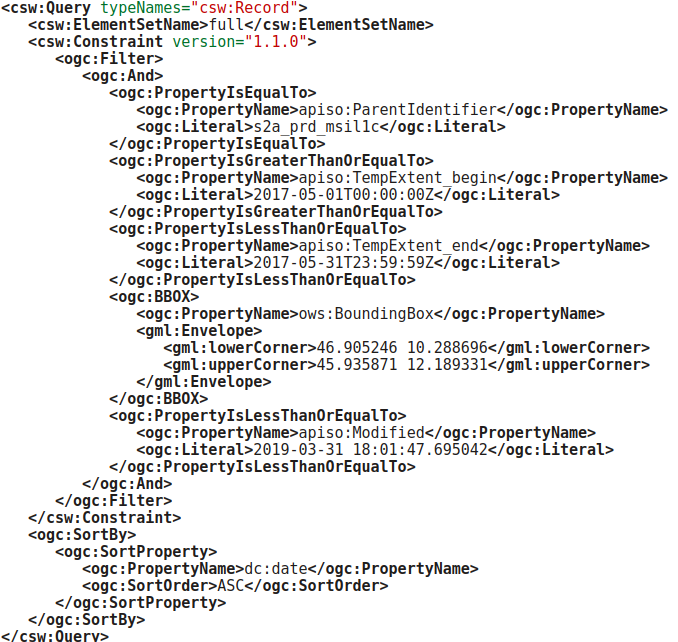
\includegraphics[width=\textwidth]{appendix_pidB}
	\caption{Original query of \textit{jobB} from the evaluation in Section \ref{Evaluation:special_dataid}.}
	\label{fig:appendix_pidB} % \label has to be placed AFTER \caption (or \subcaption) to produce correct cross-references.
\end{figure}

\begin{figure}[h]
	\centering
	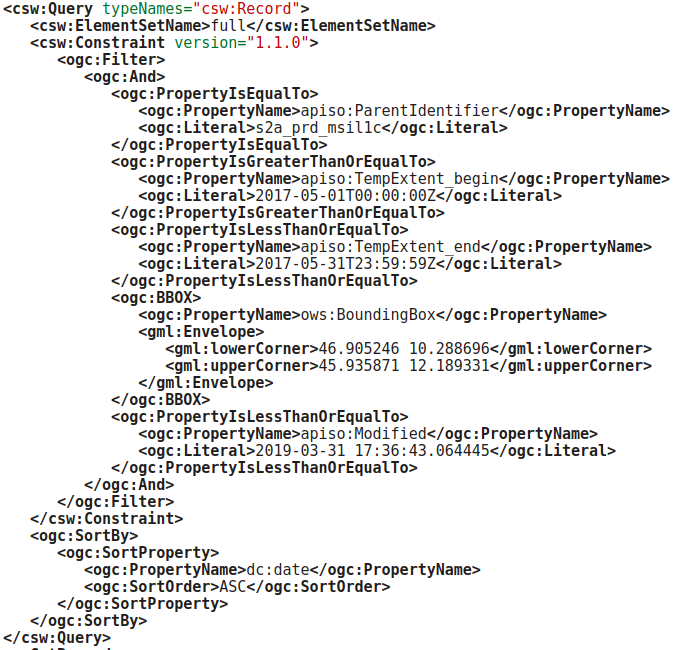
\includegraphics[width=\textwidth]{appendix_pidD}
	\caption{Original query of \textit{jobD} from the evaluation in Section \ref{Evaluation:special_dataid}.}
	\label{fig:appendix_pidD} % \label has to be placed AFTER \caption (or \subcaption) to produce correct cross-references.
\end{figure}

\backmatter


% Use an optional list of figures.
\listoffigures % Starred version, i.e., \listoffigures*, removes the toc entry.

% Use an optional list of tables.
\cleardoublepage % Start list of tables on the next empty right hand page.
\listoftables % Starred version, i.e., \listoftables*, removes the toc entry.



%\renewcommand\listoflistingscaption{List of source codes}
\listoflistings



% Use an optional list of alogrithms.
%\listofalgorithms
%\addcontentsline{toc}{chapter}{List of Algorithms}

% Add an index.
\printindex
\newpage
% Add a glossary.
\printglossaries

% Add a bibliography.
\bibliographystyle{abbrv}
\bibliography{intro}

\end{document}